\documentclass[12pt,a4paper,fleqn]{article}

\usepackage[utf8]{inputenc}
\usepackage[french]{babel}
\usepackage{tikz}
\usetikzlibrary{positioning}
\usetikzlibrary{decorations.markings}
\usepackage[T1]{fontenc}
\usepackage{amsmath}																				% les maths
\usepackage{amsfonts}
\usepackage{amssymb}
\usepackage{fourier}																					% symboles intégral propre
\usepackage{graphicx}
\usepackage[left=2cm,right=2cm,top=2cm,bottom=2cm]{geometry}	% les marges
\usepackage{multicol}																					% pour écrire sur plusieurs colones
\usepackage{setspace}																				% set space between lines
\usepackage{array}																						% stretch array lines
\usepackage[hyphens]{url}
%\usepackage[hyphenbreaks]{breakurl}														% for long urls
\usepackage{chemfig}																					% pour les formules chimiques


\usepackage[breaklinks]{hyperref}															% clickable links
\hypersetup{
    colorlinks=true,
    linkcolor=red_f,
    citecolor=bleu_f,
    filecolor=green_f,
    urlcolor=bleu_f
}

\usepackage{xcolor}																			% colors
\usepackage[framemethod=tikz]{mdframed}									% fancy environments

\usepackage{siunitx}        																% écriture des nombres et unités
\sisetup{
locale = FR,
per-mode = symbol,%reciprocal,
exponent-product = \times, % replace by \cdot if desired
exponent-mode=input,
separate-uncertainty = true,
output-complex-root = j, % or i
number-unit-product = \, ,
}

%%%%%%%%%% graphic charter

\renewcommand{\familydefault}{\sfdefault}												% sans serif font

%%%%% HEADER
%\pagestyle{fancy}
%\lhead{\textcolor{gray_f}{Physique-Chimie\\R. METZDORFF}}
%\chead{\textcolor{gray_f}{Lycée Suzanne Valadon}}
%\rhead{\textcolor{gray_f}{2020-2021}}
%\renewcommand{\headrulewidth}{0.4pt}
%\let\HeadRule\headrule
%\renewcommand\headrule{\color{gray_f}\HeadRule}

%%%%% COLORS
\definecolor{gray_f}{RGB}{68,84,106}
\definecolor{gray_c}{RGB}{214,220,229}
\definecolor{gray_cc}{RGB}{245,245,245}
\definecolor{bleu_f}{RGB}{91,155,213}
\definecolor{bleu_c}{RGB}{222,235,247}
\definecolor{red_f}{RGB}{204,0,0}
\definecolor{red_c}{RGB}{245,204,204}
\definecolor{orange_f}{RGB}{237,125,49}
\definecolor{orange_c}{RGB}{251,229,214}
\definecolor{green_f}{RGB}{112,173,71}
\definecolor{green_c}{RGB}{226,240,217}
\definecolor{yellow_f}{RGB}{255,192,0}
\definecolor{yellow_c}{RGB}{255,242,204}
\definecolor{code_keyword}{RGB}{23,23,139}										% colors for pyhton code
\definecolor{code_comment}{RGB}{50,137,21}
\definecolor{code_string}{RGB}{139,139,25}
\definecolor{red_unilim}{RGB}{166,41,41}
\definecolor{gray_unilim}{RGB}{78,87,94}
\definecolor{orange_unilim}{RGB}{209,98,40}

%%%%% NEW ENVIRONMENTS

%%% header
\mdfdefinestyle{s_head}{%
	linecolor=red_unilim!,
	outerlinewidth=3pt,%
	frametitlerule=false,
	topline=false,
	bottomline=false,
	rightline=false,
	leftline=false,
	backgroundcolor=red_unilim,
	innertopmargin=8pt,
	roundcorner=0pt,
	nobreak=true,
	fontcolor=white
}
\newmdenv[style=s_head]{header_env}
\newenvironment{header}
{%\stepcounter{exa}%
	\addcontentsline{ldf}{figure}{0}%
	\begin{header_env}\qquad\Large\bf}
	{\end{header_env}}

%%%%% New command

\newcommand{\app}{\colorbox{bleu_c}{\textcolor{bleu_f}{APP}}}
\newcommand{\rea}{\colorbox{yellow_c}{\textcolor{yellow_f}{REA}}}
\newcommand{\anarai}{\colorbox{green_c}{\textcolor{green_f}{ANA-RAI}}}
\newcommand{\val}{\colorbox{orange_c}{\textcolor{orange_f}{VAL}}}
\newcommand{\com}{\colorbox{red_c}{\textcolor{red_f}{COM}}}
\newcommand{\auto}{\colorbox{white}{\textcolor{black}{AUTO}}}
\newcommand{\rco}{\colorbox{gray_c}{\textcolor{gray_f}{RCO}}}


\bibliographystyle{custom-bib/thesis}
\usepackage{bibentry}
\usepackage{pdfpages}

\newcommand{\ex}{\vec{e}_x}
\newcommand{\ey}{\vec{e}_y}
\newcommand{\ez}{\vec{e}_z}

\renewcommand{\d}{\mathrm{d}}
\newcommand{\cad}{c'est-à-dire}

\usepackage[european, straightvoltages, RPvoltages]{circuitikz}
\usetikzlibrary{babel}

\begin{document}

\begin{header}
\begin{minipage}{0.55\textwidth}
Rapport de Master 2
\end{minipage}
\begin{minipage}{0.38\textwidth}
\href{https://www.unilim.fr/}{
\includegraphics[scale=1]{logo.png}}
\end{minipage}
\end{header}

\vspace{30pt}
\begin{spacing}{1.2}
{\bf
\begin{Large}
\noindent
\textcolor{gray_unilim}{INSPE Académie de Limoges}
\end{Large}

\begin{large}
\noindent
\textcolor{gray_unilim}{Métiers de l'enseignement, de l'éducation et de la formation}

\noindent
\textcolor{gray_unilim}{Master MEEF Second degré}

\noindent
\textcolor{gray_unilim}{Professeur de Physique et de Chimie}

\noindent
\textcolor{gray_unilim}{Didactique, épistémologie et histoire des sciences}

\end{large}
}

\vspace{20pt}

\noindent
\textcolor{gray_unilim}{2020--2021}

\vspace{40pt}
\begin{large}
\bf
\noindent
\textcolor{gray_unilim}{Galvanomètres}

\vspace{150pt}
\noindent
\textcolor{gray_unilim}{Antoine \textsc{Eggenspiller}}

\noindent
\textcolor{gray_unilim}{Collège Guy de Maupassant}

\vspace{\baselineskip}

\noindent
\textcolor{gray_unilim}{Rémi Metzdorff}

\noindent
\textcolor{gray_unilim}{Lycée Suzanne Valadon}
\end{large}
\end{spacing}

\vfill

\hfill

\includegraphics[scale=1]{logo_bottom.png}

\thispagestyle{empty}
\newpage

\tableofcontents
\newpage



\section*{Introduction}
\addcontentsline{toc}{section}{Introduction}

Ce rapport présente le fonctionnement et la restauration de deux galvanomètres datant du début du XX\textsuperscript{ème} siècle.
Il s'agit d'un ampèremètre et d'un voltmètre produits par Chauvin \& Arnoux.
Les détails concernant l'historique de ces appareils sont présentés extensivement dans un précédent rapport \cite{Ardellier2016} et ne seront pas repris ici.
La première section s'intéresse au principe de fonctionnement du galvanomètre et en présente un modèle simplifié.
La restauration des deux appareils est ensuite détaillée.
Finalement, une expérience simple impliquant les deux instruments est présentée.


\section{Principe de fonctionnement}

\subsection{Principe général}

\begin{figure}[htbp]
    \center
    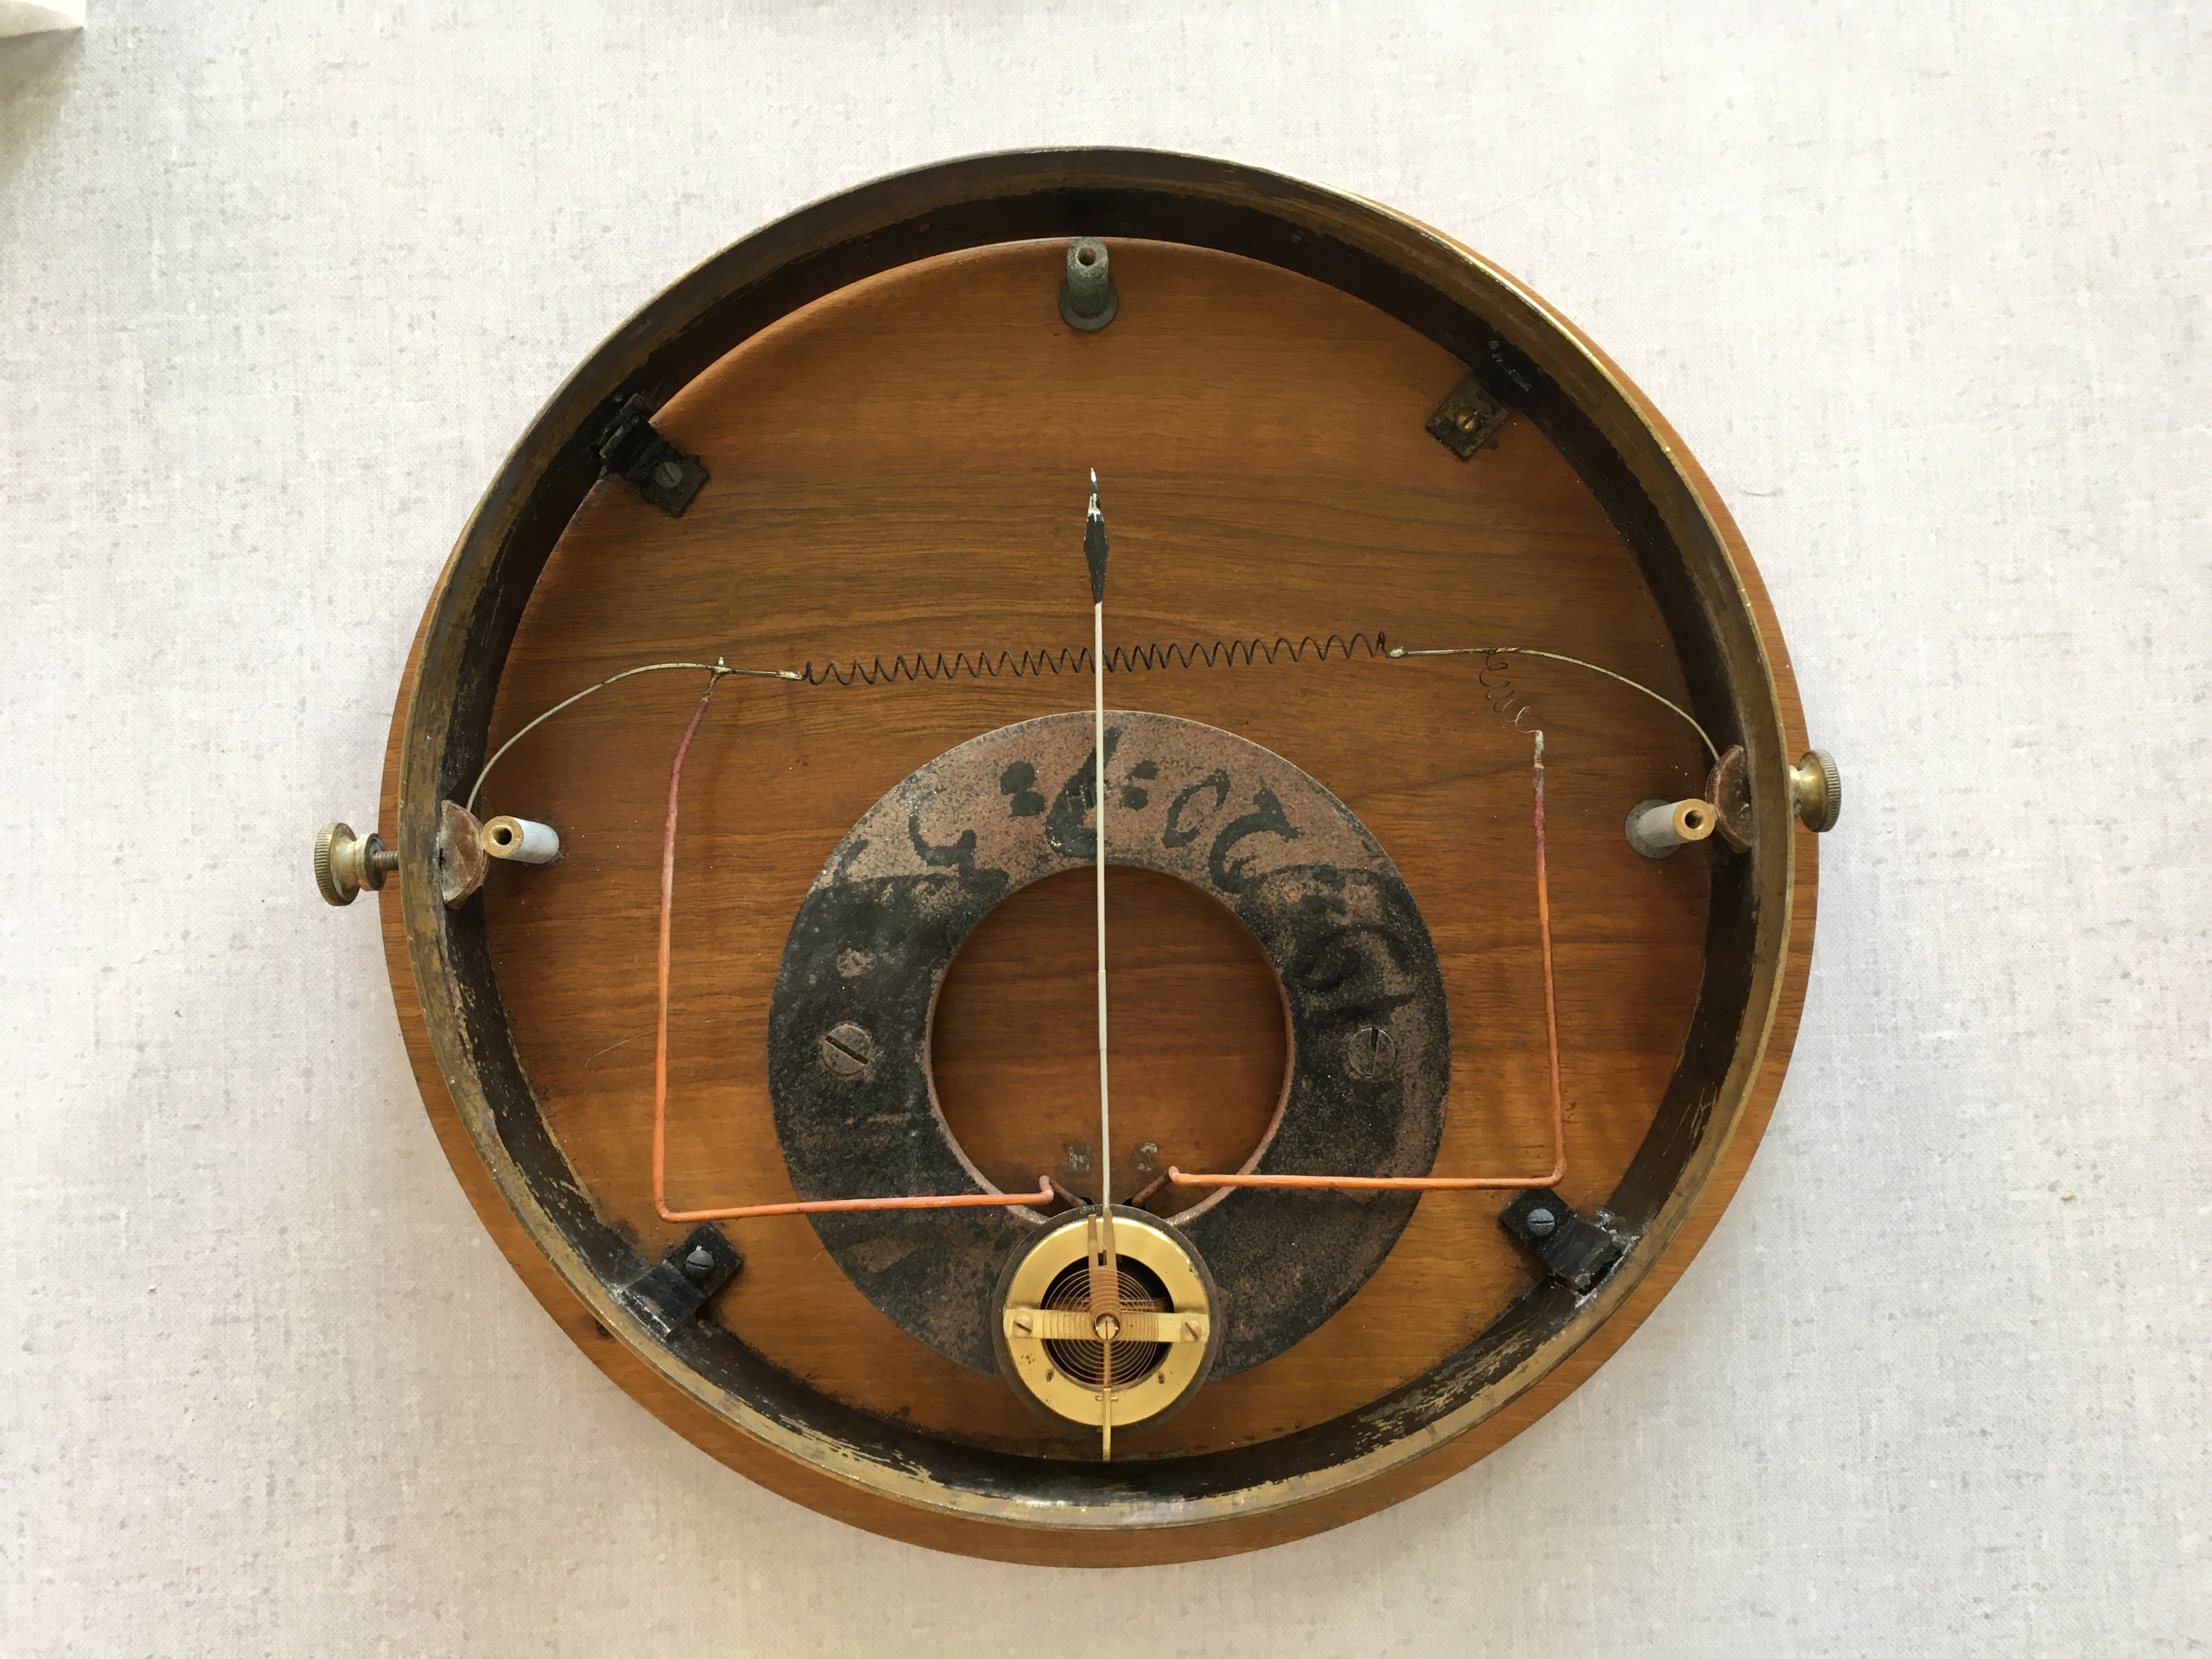
\includegraphics[trim=1300 300 1300 800, clip, width=.5\linewidth]{images/IMG_4037.JPG}
    \caption{
    Le \og cœur \fg{} du galvanomètre.
    Le champ magnétique est produit par l'aimant permanent torique.
    La cadre mobile, situé dans l'entrefer de l'aimant, est caché derrière un ressort en spirale qui maintient l'aiguille au centre du cadran en l'absence de courant électrique.
    Les deux fils situés de part et d'autre du cadre alimentent la bobine.
    Le fil noir fin en forme de ressort est propre à l'ampèremètre : il n'est pas indispensable au fonctionnement du galvanomètre et son rôle sera expliqué plus tard.}
    \label{fig:principe}
\end{figure}

Il existe plusieurs types de galvanomètres adaptés à différents usages.
Ceux présentés ici sont dit à \emph{cadre mobile}.
\og \emph{Ces galvanomètres sont basés sur le principe d'un cadre galvanométrique mobile dans un champ magnétique produit par un aimant permanent} \fg{}, comme l'explique la notice du fabriquant (Ann.~\ref{ann:catalogue}).
Le cadre galvanométrique est un circuit qui prend la forme d'une bobine de fil de cuivre : lorsqu'elle est parcourue par un courant $I$, l'action du champ magnétique se traduit par une force de Laplace, proportionnelle à $I$, qui s'exerce sur chaque élément du circuit.
La construction de l'instrument autorise simplement le cadre à pivoter.
Celui-ci est lié à une aiguille qui permet de mesurer sa déviation et ainsi de mesurer le courant qui passe à travers la bobine (Fig.~\ref{fig:principe}).
Ce type d'instrument ne permet de mesurer que des courants et tensions continus mais a l'avantage d'être très précis.
Pour des mesures en courant alternatif, on utilisera plutôt des galvanomètres à palettes par exemple.

Le galvanomètre est donc un instrument qui permet de mesurer un courant électrique.
L'ampèremètre fonctionne exactement sur ce principe : branché en série dans le circuit, la bobine est parcourue par le courant qui circule dans la branche mesurée.
\footnote{On le verra, la réalisation pratique de l'instrument est un peu plus subtile, ce qui permet de mesurer des courants d'intensités variées.} 
Le voltmètre contient des résistances supplémentaires de valeurs relativement élevées : branché en parallèle aux bornes d'un dipôle, l'appareil et sa bobine sont parcourus par un courant faible qu'il est possible de mesurer.
\footnote{Le courant qui parcourt l'instrument doit être beaucoup plus faible que celui qui traverse le dipôle de manière à perturber le moins possible le circuit : la résistance du voltmètre doit être aussi grande que possible.
Toutefois, le courant passant à travers la bobine doit être suffisant pour que l'action des forces de Laplace conduise à une déviation significative de l'aiguille.
Il y a donc un compromis à trouver.}

La modélisation du fonctionnement de l'appareil s'est avérée plus subtile que ce qui avait été anticipé.
On commence ici par un premier modèle simple qui a le mérite de détailler le principe de fonctionnement de l'appareil.
Les résultats obtenus ne sont cependant pas en accord avec les observations réalisées sur les instruments, comme nous le verrons plus tard : il sera donc nécessaire d'apporter plusieurs améliorations au modèle initialement choisi.
Ce cheminement a toutefois permis de comprendre plusieurs aspects importants liés à la conception du galvanomètre à cadre mobile.

\subsection{Modélisation}

Tout d'abord, on souhaite décrire le mouvement de la bobine parcourue par un courant $I$ dans le champ magnétique $\vec{B}=B\vec{e}_x$ supposé uniforme, qui règne dans l'entre-fer de l'aimant.
Le problème est similaire à celui du pendule de torsion soumis à un couple constant, en présence de frottements fluides.
On s'intéresse au seul degré de liberté $\theta$ du système, qui correspond à l'angle algébrique entre le champ $\vec{B}$ et le vecteur $\vec{n}$ normal aux spires de la bobine.

\begin{multicols}{3}
    \begin{center}
        \begin{tikzpicture}[scale=1]
            \draw[thick] (0,0,-2) -- (0,0,2);
            \filldraw[white] (0,0) ellipse (1 and .4);
            \draw[thick] (0,0) ellipse (1 and .4);
            \draw[ultra thick, decorate, decoration={markings,mark=at position 0.75 with{\arrow[black]{stealth}};}] (0,0) ellipse (1 and .4);
            \draw (0, -.4) node[below] {$I$};
            \draw[thick,->,>=stealth,blue] (0,0) --++ (0,1) node[left]{$\vec{n}$};

            \coordinate (B) at (2,0);
            \draw[red] (B) + (0.5,0) node[below]{$\vec{B}$};
            \draw[thick,->,>=stealth,red] (B) --++ (1,0);
        \end{tikzpicture}

        Courant nul : $I=0$.

        \begin{tikzpicture}[scale=1]
            \draw[thick] (0,0,-2) -- (0,0,2);
            \filldraw[white,rotate=-30] (0,0) ellipse (1 and .4);
            \draw[thick,rotate=-30] (0,0) ellipse (1 and .4);
            \draw[ultra thick,rotate=-30, decorate, decoration={markings,mark=at position 0.85 with{\arrow[black]{stealth}};}] (0,0) ellipse (1 and .4);
            \draw (0, -.5) node[below] {$I$};

            \draw[thick,->,>=stealth,blue] (0,0) --++ (60:1) node[left]{$\vec{n}$};

            \coordinate (B) at (2,0);
            \draw[red] (B) + (0.5,0) node[below]{$\vec{B}$};
            \draw[thick,->,>=stealth,red] (B) --++ (1,0);
        \end{tikzpicture}

        Courant non nul : $I\neq0$.

        \begin{tikzpicture}[scale=1]
            \coordinate (O) at (-0,0);
            \draw[gray] (O) node [left] {$O$};
            \draw [gray] [->,>=stealth] (O) --++(1,0,0) node [below] {$x$};
            \draw [gray] [->,>=stealth] (O) --++(0,1,0) node [left] {$y$};
            \draw [gray] [->,>=stealth] (O) --++(0,0,1) node [below] {$z$};

            \draw[thick,->,>=stealth,blue] (O) --++ (60:1) node[above right]{$\vec{n}$};
            \draw[thick,->,>=stealth] (O)+(.5,0) arc (0:60:.5);
            \draw (O)+(30:.5) node[right]{$\theta$};
        \end{tikzpicture}

        Conventions utilisées.
    \end{center}
\end{multicols}

\subsubsection{Équations du mouvement}

Le système étudié est l'ensemble \{bobine + aiguille\}.
La bobine est supposé plate, rectangulaire de côtés $a$ et $b$ délimitant une surface $S$ et formée de $N$ spires parcourue par un courant constant d'intensité $I$ dont l'orientation définit celle du vecteur $\vec{n}$ normal à la surface $S$.
On l'assimile à un dipôle magnétique dont le moment est $\vec{\mu} = NSI\vec{n}$.
L'ensemble bobine et aiguille possède par ailleurs un moment d'inertie $J$.

Le temps caractéristique de l'évolution du système est au plus de l'ordre de quelques secondes.
Le référentiel du laboratoire peut donc être considéré comme galiléen.

Plusieurs forces doivent être considérées :
\begin{itemize}
    \item le poids : au mieux, son moment est nul, mais au pire, il est négligé \footnote{Cette approximation semble raisonnable compte tenu de la très grande légèreté de l'aiguille.
    Le reste du cadre est centré autour de son axe de rotation et n'ajoute donc aucun couple.} ;
    \item $\vec{\Gamma}_B = \vec{\mu} \wedge \vec{B} = - \mu B \sin \theta \ez$ : moment subi par le dipôle magnétique $\vec{\mu}$ dans le champ $\vec{B}$ (moment des forces de Laplace) ;
    \item $\vec{\Gamma}_H = -k(\theta-\pi/2)\ez$ : moment de la force de rappel du ressort spiral ;
    \item $\vec{\Gamma}_f = -\alpha\dot{\theta}\ez$ : moment des forces de frottement.
    On choisit ici de ne considérer que des frottements fluides.
    \footnote{
        La modélisation de ces frottements n'est pas essentielle puisqu'on ne s'intéresse qu'au cas statique.
        Toutefois, la présence de frottements solides peut conduire à un phénomène d'hystérésis qui modifie la position d'équilibre de l'aiguille.
        Cependant, avec les appareils utilisés ici, les mesures ne montrent pas d'hystérésis important ce qui justifie cette approximation.}
\end{itemize}

Le moment cinétique de l'ensemble bobine et aiguille $\vec{L} = J\dot{\theta}\ez$ s'exprime en fonction du moment d'inertie $J$ du système.
On applique le théorème du moment cinétique :
\begin{equation}
    \frac{\d\vec{L}}{\d t} 	= \vec{\Gamma}_B + \vec{\Gamma}_H + \vec{\Gamma}_f,
\end{equation}
et on le projette selon $\ez$ :
\begin{equation}
    J\ddot{\theta} = -\mu B \sin \theta - k\left(\theta-\frac{\pi}{2}\right) - \alpha\dot{\theta}.
    \label{eq:mvt}
\end{equation}

Cette équation comprend un terme en $\sin\theta$ : elle n'est pas linéaire et ne pourra pas être résolue analytiquement.
Pour simplifier, on peut réaliser des approximations supplémentaires en supposant que la déviation reste faible, \cad{} que $\theta$ reste \og proche \fg{} de $\tfrac{\pi}{2}$.
On peut alors linéariser l'équation~\ref{eq:mvt} pour obtenir l'équation
\begin{equation}
    J\ddot{\theta} = -\mu B - k\left(\theta-\frac{\pi}{2}\right) - \alpha\dot{\theta}.
    \label{eq:mvt_lin}
\end{equation}
Une approximation moins brutale peut aussi être obtenue en effectuant un développement limité à l'ordre deux :
\begin{equation}
    J\ddot{\theta} = - \mu B \left[ 1-\frac{\left(\theta-\frac{\pi}{2}\right)^2}{2} \right] - k\left(\theta-\frac{\pi}{2}\right) - \alpha\dot{\theta}.
    \label{eq:mvt_dl}
\end{equation}

La résolution de ces équations en régime permanent, \cad{} quand $\ddot{\theta}$ et $\dot{\theta}$ sont nuls, permet d'obtenir la position d'équilibre de l'aiguille et donc la déviation correspondant à la mesure réalisée.

\subsubsection{Position d'équilibre}

Dans le cas le plus simple, on utilise l'équation~\ref{eq:mvt_lin} qui se simplifie et on trouve l'expression de la position d'équilibre $\theta_\mathrm{eq}^\mathrm{lin}$ du système :
\begin{equation}
    \theta_\mathrm{eq}^\mathrm{lin} = \frac{\pi}{2} - \frac{\mu B}{k},
    \label{eq:sol_lin}
\end{equation}
valable pour de faibles déviations, \cad{} tant que $\frac{\mu B}{k} \ll 1$.

Quand on utilise le développement limité, la résolution de l'équation~\ref{eq:mvt_dl} en régime permanent fait apparaitre deux solutions, dont l'une diverge pour les petites valeurs de $\tfrac{\mu B}{k}$.
L'autre donne finalement :
\begin{equation}
    \theta_\mathrm{eq}^\mathrm{DL2} = \frac{\pi}{2} + \frac{1-\sqrt{1+2\left(\frac{\mu B}{k}\right)^2}}{\frac{\mu B}{k}}.
    \label{eq:sol_dl}
\end{equation}
Lorsque $\frac{\mu B}{k} \ll 1$, on peut linéariser cette solution et on retrouve bien la position d'équilibre précédente, obtenue dans le cas de très faibles déviations.

L'équation~\ref{eq:mvt} en régime permanent s'écrit
\begin{equation}
    0 = -\mu B \sin \theta - k\left(\theta-\frac{\pi}{2}\right),
    \label{eq:sol_num}
\end{equation}
et n'admet pas de solution analytique.
Il est toutefois possible de la résoudre numériquement pour obtenir $\theta_\mathrm{eq}^\mathrm{num}$.

Dans la suite, on repèrera la position d'équilibre par sa déviation $D$, avec
\begin{equation}
    D = \frac{\pi}{2} - \theta,
\end{equation}
qui correspond, à un facteur d'échelle près, à la valeur lue sur les galvanomètres.


\subsubsection{Linéarité de l'affichage}

\begin{figure}[htbp]
    \center
    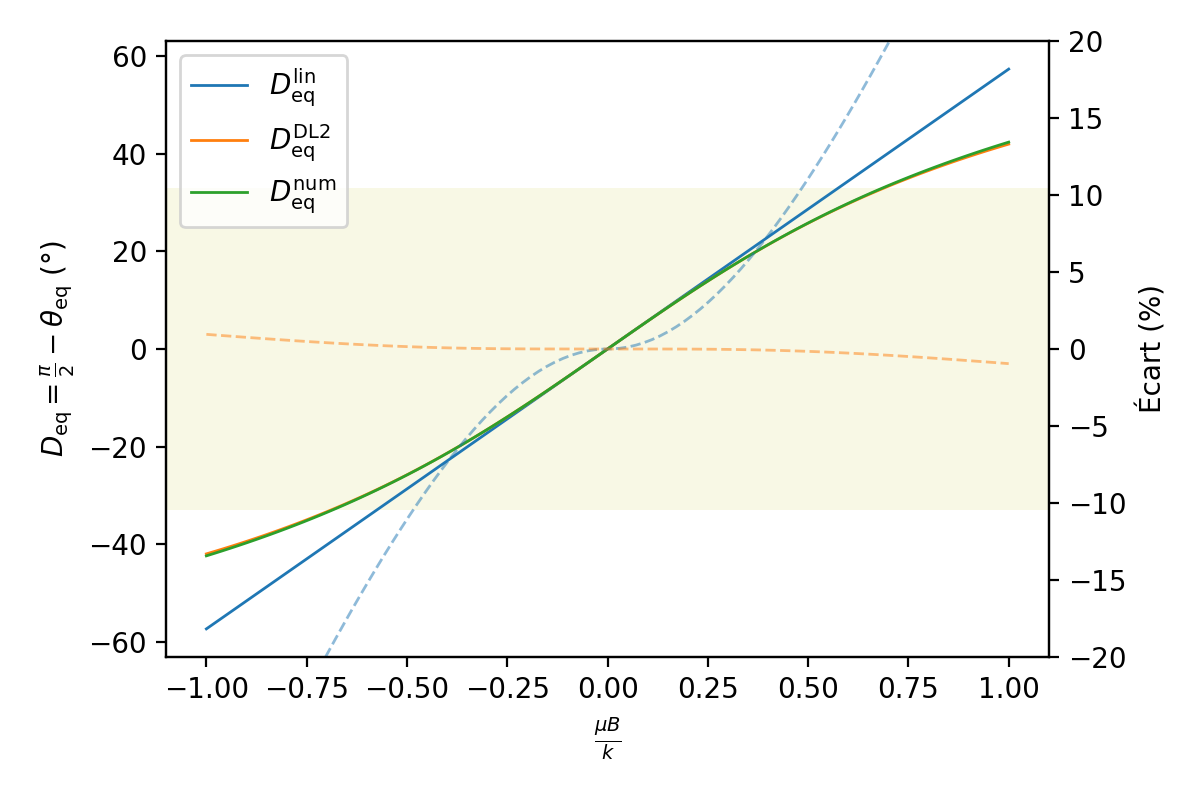
\includegraphics[scale=1]{deviation.png}
    \caption{Déviation de l'aiguille du galvanomètre en fonction du rapport $\tfrac{\mu B}{k}$ proportionnel au courant mesuré.
Les trois courbes pleines représentent les déviations associées aux trois solutions obtenues précédemment dans le cadre de l'approximation linéaire, du développement limité au second ordre et de la résolution numérique.
Les courbes en pointillés montrent l'écart relatif entre les déviations calculées analytiquement (Éq.~\ref{eq:sol_lin} et \ref{eq:sol_dl}) et la résolution numérique (Éq.~\ref{eq:sol_num}).
La plage de déviations matérialisée en jaune pâle représente la gamme de valeurs effectivement mesurables par l'instrument, compte tenu de l'amplitude de mouvement de l'aiguille.}
    \label{fig:deviation}
\end{figure}

La comparaison des solutions obtenues avec différentes approximations (Fig.~\ref{fig:deviation}) montre que la solution analytique $\theta_\mathrm{eq}^\mathrm{DL2}$ obtenue en faisant un développement limité à l'ordre deux (Éq.~\ref{eq:sol_dl}) permet d'obtenir une excellente approximation de la position d'équilibre du système sur la plage de mesure accessible à l'instrument.
En effet, l'écart relatif avec la valeur calculée numériquement reste inférieur à \SI{0.4}{\percent} sur l'ensemble de la plage de mesure.
En revanche, l'approximation linéaire donne un écart relatif inférieur à \SI{1}{\%} pour des déviations inférieures à \SI{8}{\degree}, mais proche de \SI{20}{\%} au maximum de déviation.

On s'attend donc à une déviation de l'aiguille sensiblement plus faible que celle attendue si la déviation était proportionnelle au courant $I$.
Cet écart est parfaitement compréhensible dans notre modèle où la force de rappel du ressort est proportionnelle à l'angle $\theta$ alors que le moment magnétique $\Gamma_B$ s'affaiblit à mesure que le dipôle magnétique s'aligne avec le champ de l'aimant permanent.

\subsubsection{Validité du modèle}

\begin{figure}[htbp]
    \center
    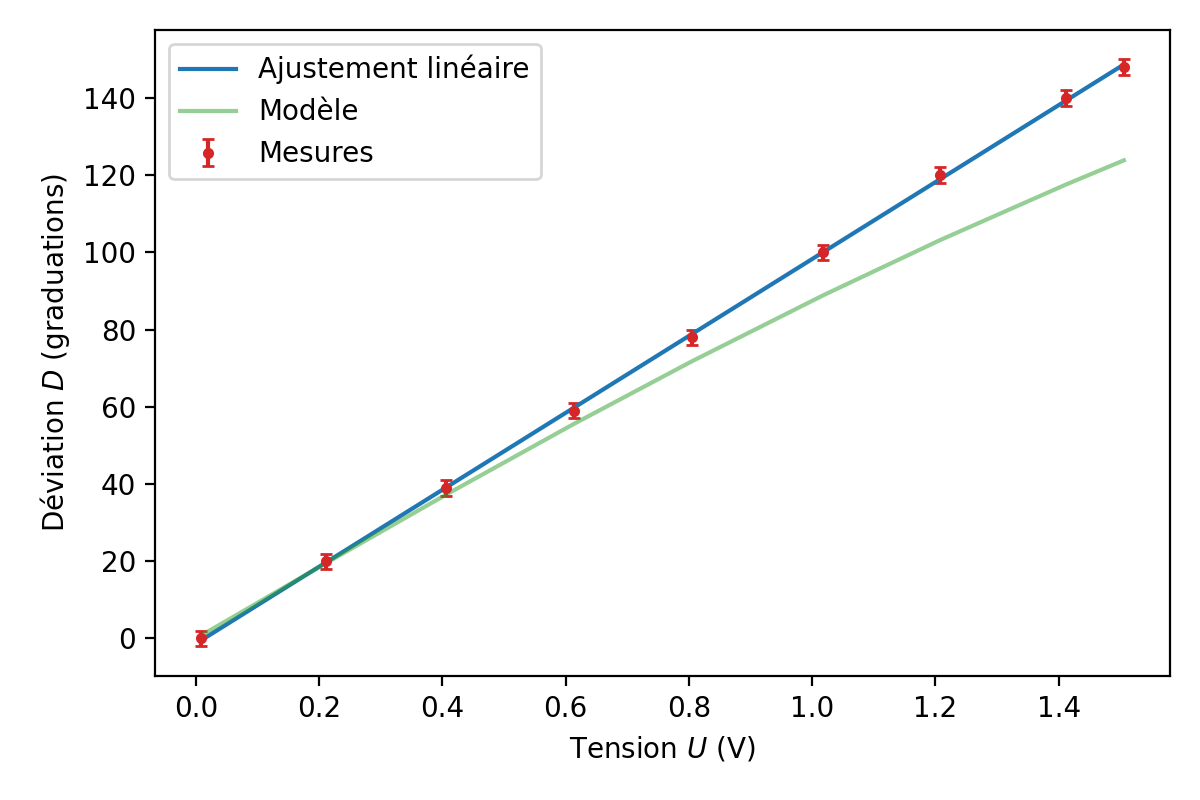
\includegraphics[scale=1]{images/galva_lin.png}
    \caption{Mesure de la déviation en fonction de la tension aux bornes du galvanomètre voltmètre.
    La tension d'une alimentation stabilisée est modifiée et mesurée simultanément à l'aide du galvanomètre et d'un multimètre numérique pour reconstituer la courbe.
    Le calibre du galvanomètre est choisi pour explorer l'ensemble des déviations mesurables.
    De manière surprenante, l'ajustement linéaire semble excellent ($\chi^2_\mathrm{r} \approx \num{0.1}$, $r\approx\num{0.9998}$), y compris aux \og grandes \fg{} valeurs de déviation.
}
    \label{fig:galva_lin}
\end{figure}

Des mesures rapides effectuées sur les différents appareils ont cependant montré que le comportement de l'appareil était très linéaire (Fig~\ref{fig:galva_lin}).
\footnote{La linéarité des graduations sur les cadrans des instruments a été vérifiée à l'aide d'un réglet.}
On peut donc tenter de revenir sur les différentes hypothèses utilisées pour établir le modèle précédent :
\begin{itemize}
\item uniformité du champ $\vec{B}$ : cette approximation reste valable tant que l'on reste à proximité de l'axe de l'entrefer de l'aimant permanent (Fig.~\ref{fig:entrefer}).
Cependant, puisque la taille du cadre mobile est comparable à celle de l'entrefer, pour des déviations importantes, la bobine explore des régions sensiblement éloignées de l'axe de l'entrefer.
À mesure que l'on s'éloigne de cet axe, le champ magnétique diminue.
Quand l'intensité $I$ est faible, la bobine est proche de l'axe ($\theta\approx\tfrac{\pi}{2}$) et elle s'en éloigne quand l'intensité augmente : le couple magnétique devrait donc également diminuer à mesure que la déviation augmente.
Cet effet, qui s'ajoute à la diminution du couple à mesure que le dipôle s'aligne avec le champ, devrait en réalité augmenter la non linéarité de l'affichage et ne convient pas pour expliquer les mesures réalisées ;
\begin{figure}[htbp]
    \center
    \begin{tikzpicture}
        \shade[left color=gray_f!25, right color=gray_f!100] (-4,1) --++ (2,0) --++(0,-2) --++ (-2,0);
        \shade [left color=gray_f!100, right color=gray_f!25] (4,1) --++ (-2,0) --++(0,-2) --++ (2,0);
        \foreach \i in {0,1,...,6} {
            \pgfmathsetmacro\h{-1 +1*\i / 3}
	        \coordinate (A) at (-2,\h);
            \coordinate (B) at (2,\h);
	       \draw[color=red] (A) to[bend left=20*\h] (B);
	       \draw[thick,decorate, decoration={markings,mark=at position 0.5 with{\arrow[red]{stealth}};}] (A) to[bend left=20*\h] (B);
	   }
    \end{tikzpicture}
    \caption{Représentation schématique de quelques lignes de champ au niveau de l'entrefer de l'aimant permanent.}
    \label{fig:entrefer}
\end{figure}

\item poids négligeable : dans le cas où l'on devrait considérer le poids de l'aiguille, il faudrait rajouter à l'équation~\ref{eq:mvt} un terme en $\cos\theta$ correspondant au couple du poids, dont la valeur est par ailleurs difficile à estimer sans démonter complètement l'appareil.
On obtient alors l'équation 
\begin{equation}
J\ddot{\theta} = -\mu B \sin \theta - k\left(\theta-\frac{\pi}{2}\right) - \alpha\dot{\theta} - \beta \cos\theta,
\label{eq:mvt_poids}
\end{equation}
où $\beta$ est lié au poids de l'aiguille.
A priori, ce terme pourrait convenir : au contraire du moment magnétique, sa valeur augmente avec la déviation et pourrait ainsi compenser la diminution du moment magnétique.
La résolution numérique de l'équation \ref{eq:mvt_poids} dans le régime statique pour plusieurs valeurs de $\beta$ ne laisse cependant pas apparaitre d'amélioration significative.
De plus, les galvanomètres affichent des valeurs identiques, qu'ils soient disposés verticalement ou horizontalement, en accord avec les annonces du fabriquant : \og \emph{Ces galvanomètres fonctionnent dans toutes les positions et sous n'importe quelle orientation} \fg{} (Ann.~\ref{ann:catalogue}). 
\footnote{Le support des galvanomètres les destine à être orientés verticalement (aiguille vers le haut), ce qui a conduit à l'hypothèse selon laquelle le poids de l'aiguille joue un rôle dans la mesure.}
L'approximation réalisée en négligeant le poids semble donc également raisonnable ;

\item force de rappel du ressort spirale : une dépendance plus complexe qu'une simple proportionnalité n'est pas impossible mais il semble que ce type de ressort soit l'un des rares qui ait un \og comportement vraiment linéaire \fg{} \cite{wiki_ressort} ;

\item géométrie de la bobine : le cadre mobile a une géométrie plus complexe que celle envisagée dans le modèle.
Les détails sont toutefois difficiles à prendre en compte sans rentrer dans une démarche qui dépasse le cadre de ce travail.
Il est par ailleurs difficile d'imaginer que ces détails améliorent la linéarité de l'affichage.
\end{itemize}

\subsubsection{Et avec un entrefer concave ?}

Dans ce qui précède, la forme de l'entrefer est très simple (Fig.~\ref{fig:entrefer}).
Toutefois, il est possible de considérer une forme plus évoluée, adaptée à un cadre mobile pivotant (Fig.~\ref{fig:entrefer_cyl}).
\footnote{Sur les instruments utilisés, la forme précise de l'entrefer est difficile à apercevoir sans démonter davantage l'appareil.
Toutefois, elle n'est clairement pas rectangulaire (Fig.~\ref{fig:entrefer}).}
On suppose toujours que le champ magnétique dans l'entrefer est orienté uniquement selon $\ex$ (la convention pour l'orientation des axes reste la même qu'avant).
\footnote{Cette approximation est discutable mais reste raisonnable tant que l'on reste assez proche de l'axe de l'entrefer.}
Le champ magnétique n'est cependant plus uniforme car l'épaisseur $e(\nu)$ de l'entrefer change et dépend de la distance par rapport à l'axe : on peut le noter $B(\nu)\ex$.
Pour calculer le champ magnétique $B(\nu)$, on procède par analogie avec le calcul du champ dans l'entrefer d'un électroaimant \cite{Faroux1998}.
Il apparait que le champ $B$ est inversement proportionnel à l'épaisseur $e(\nu)=2r\cos\nu$.
Ici on a donc
\begin{equation}
B(\nu) \propto \frac{1}{\cos\nu}.
\end{equation}

\begin{figure}
\center
\begin{tikzpicture}
\newcommand{\radius}{2}
\newcommand{\angopen}{60}
\coordinate (O) at (0:0);
\pgfmathsetmacro\h{\radius*sin(\angopen)}
\draw[dashed] (O) circle (\radius);
\shade[left color=gray_f!25, right color=gray_f!100]  (-2*\radius, \h) -- (180-\angopen:\radius) arc (-\angopen:\angopen:-\radius) -- (-2*\radius, -\h);
\shade[left color=gray_f!100, right color=gray_f!25] (2*\radius, \h) -- (\angopen:\radius) arc (\angopen:-\angopen:\radius) -- (2*\radius, -\h);
\draw (O) node {$\bullet$} node [below left] {$O$} -- (25:\radius) node [midway, above left]{$r$};
\draw[thick,->,>=stealth] (O)+(1,0) arc (0:25:1);
\draw (O)+(10:1) node[right]{$\nu$};
\draw[dashed] (-2.5*\radius, 0) -- (2.5*\radius, 0);
\pgfmathsetmacro\x{\radius*cos(25)}
\pgfmathsetmacro\y{\radius*sin(25)}
\draw[gray, <->, >=stealth] (-\x, \y) -- (\x,\y) node [midway, above] {$e(\nu)$};

\draw [] (-1.5*\radius, \h/2) node {\textbf{N}};
\draw [] (1.5*\radius, \h/2) node {\textbf{S}};

\coordinate (O) at (8,0,0);
\pgfmathsetmacro\x{.9*\radius*cos(25)}
\pgfmathsetmacro\y{.9*\radius*sin(25)}

\draw[thick] (O) ++ (0,0,-2) --++ (0,0,1);
\draw[thick] (O) ++ (0,0,1) --++ (0,0,1);
\draw[thick, red] (O) ++ (\x, \y,-\radius/2) --++ (0,0,\radius);
\draw[thick] (O) ++ (\x,\y,\radius/2) --++ (-2*\x, -2*\y,0);
\draw[thick, blue] (O) ++ (-\x,-\y,\radius/2) --++ (0,0, -\radius);
\draw[thick] (O) ++ (-\x,-\y,-\radius/2) --++ (2*\x, 2*\y,0);
\draw[thick, decorate, decoration={markings,mark=at position 0.5 with{\arrow[red]{stealth}};}] (O) ++ (\x, \y,\radius/2) --++ (0,0,-\radius);
\draw[thick, decorate, decoration={markings,mark=at position 0.5 with{\arrow[blue]{stealth}};}] (O) ++ (-\x, -\y,-\radius/2) --++ (0,0,\radius);
\end{tikzpicture}
\caption{Un entrefer plus travaillé pourrait expliquer la linéarité du galvanomètre.}
\label{fig:entrefer_cyl}
\end{figure}

Le couple des forces de Laplace se calcule en considérant cette fois le cadre mobile comme une bobine formée de $N$ spires carrées de côté $l$, dont l'inclinaison est repérée par l'angle $\nu$. 
La résultante des forces de Laplace qui s'exercent sur un fil de la branche rouge parcourue par un courant $I$ (Fig.~\ref{fig:entrefer_cyl}) s'écrit $-IlB(\nu)\ey$ dont le moment est $-\frac{Il^2B(\nu)}{2}\cos(\nu)\ez$.
Le couple exercé sur le cadre mobile est donc
\footnote{Cette fois, on obtient un terme en cosinus mais cela est simplement dû à la définition de l'angle utilisé pour repérer l'inclinaison du cadre mobile : en effet, $\theta = \nu + \pi/2$.}
\begin{equation}
\vec{\Gamma}_B = -NIl^2B(\nu)\cos(\nu)\ez.
\end{equation}
En utilisant le résultat précédent concernant la dépendance du champ $\vec{B}$ avec l'angle $\nu$, on obtient finalement
\begin{equation}
\vec{\Gamma}_B \propto NIl^2 \ez,
\end{equation}
où le facteur de proportionnalité dépend simplement de l'aimantation de l'aimant permanent.

Cette équation est remarquable puisque cette fois, le moment magnétique ne dépend pas de l'inclinaison du cadre !
L'équation du mouvement (Éq.~\ref{eq:mvt}) devient linéaire, sa résolution analytique en régime permanent est alors possible et conduira à une déviation proportionnelle à l'intensité qui parcours le galvanomètre.
Avec ce dernier modèle, on explique très bien les résultats obtenus expérimentalement (Fig.\ref{fig:galva_lin}).

\subsubsection{Le noyau en fer doux}

\begin{figure}[htbp]
\center
\begin{tikzpicture}
\newcommand{\radius}{2}
\newcommand{\angopen}{60}
\coordinate (O) at (0:0);
\pgfmathsetmacro\h{\radius*sin(\angopen)}
\shade[left color=gray_f!25, right color=gray_f!100]  (-2*\radius, \h) -- (180-\angopen:\radius) arc (-\angopen:\angopen:-\radius) -- (-2*\radius, -\h);
\shade[left color=gray_f!100, right color=gray_f!25] (2*\radius, \h) -- (\angopen:\radius) arc (\angopen:-\angopen:\radius) -- (2*\radius, -\h);

\draw [] (-1.5*\radius, \h/2) node {\textbf{N}};
\draw [] (1.5*\radius, \h/2) node {\textbf{S}};

\fill [gray_c] (O) circle (.8*\radius);
\draw (O) node {Fer doux};

\foreach \x in {-50, -40,...,50} {
    \draw[red, thick] (\x:.8*\radius) -- (\x:\radius);
    \draw[thick, decorate, decoration={markings,mark=at position 0.75 with{\arrow[red]{stealth}};}] (\x:.8*\radius) -- (\x:\radius);
    \draw[red, thick] (180+\x:\radius) -- (180+\x:.8*\radius);
    \draw[thick, decorate, decoration={markings,mark=at position 0.75 with{\arrow[red]{stealth}};}] (180+\x:\radius) -- (180+\x:.8*\radius);
}
\draw[red] (55:.9*\radius) node [above left] {$\vec{B}$};
\end{tikzpicture}
\caption{La présence d'un noyau en fer doux simplifie les choses !}
\label{fig:fer_doux}
\end{figure}

Dans le cas où un noyau de fer doux est présent dans l'entrefer de l'aimant (Fig.~\ref{fig:fer_doux}), la situation est encore plus simple \cite{moving_coil}.
Dans la zone où évolue le cadre mobile :
\begin{itemize}
\item le champ magnétique est radial, donc le couple $\vec{\Gamma}_B$ est simplement proportionnel à $\vec{B}$ ;
\item l'espace entre l'aimant et le fer doux est partout le même, donc $B$ ne dépend pas de $\nu$ ;
\item l'épaisseur de l'entrefer est réduite par rapport au cas précédent : avec le même aimant permanent, le champ magnétique sera plus intense ce qui augmente la sensibilité de l'appareil.
\end{itemize}

L'inspection de l'appareil semble aller dans ce sens, puisque l'on observe bien un bloc cylindrique dans l'entrefer de l'aimant permanent sur nos appareils, autour duquel le cadre mobile est libre de bouger (Fig.~\ref{fig:theproof}).
Cette conception se rapproche fortement de celle des machines synchrones, où l'on retrouve les mêmes géométries qui permettent de façonner le champ magnétique, pour améliorer l'efficacité de ces moteurs \cite{Cardini2017}.

\begin{figure}[htbp]
    \center
    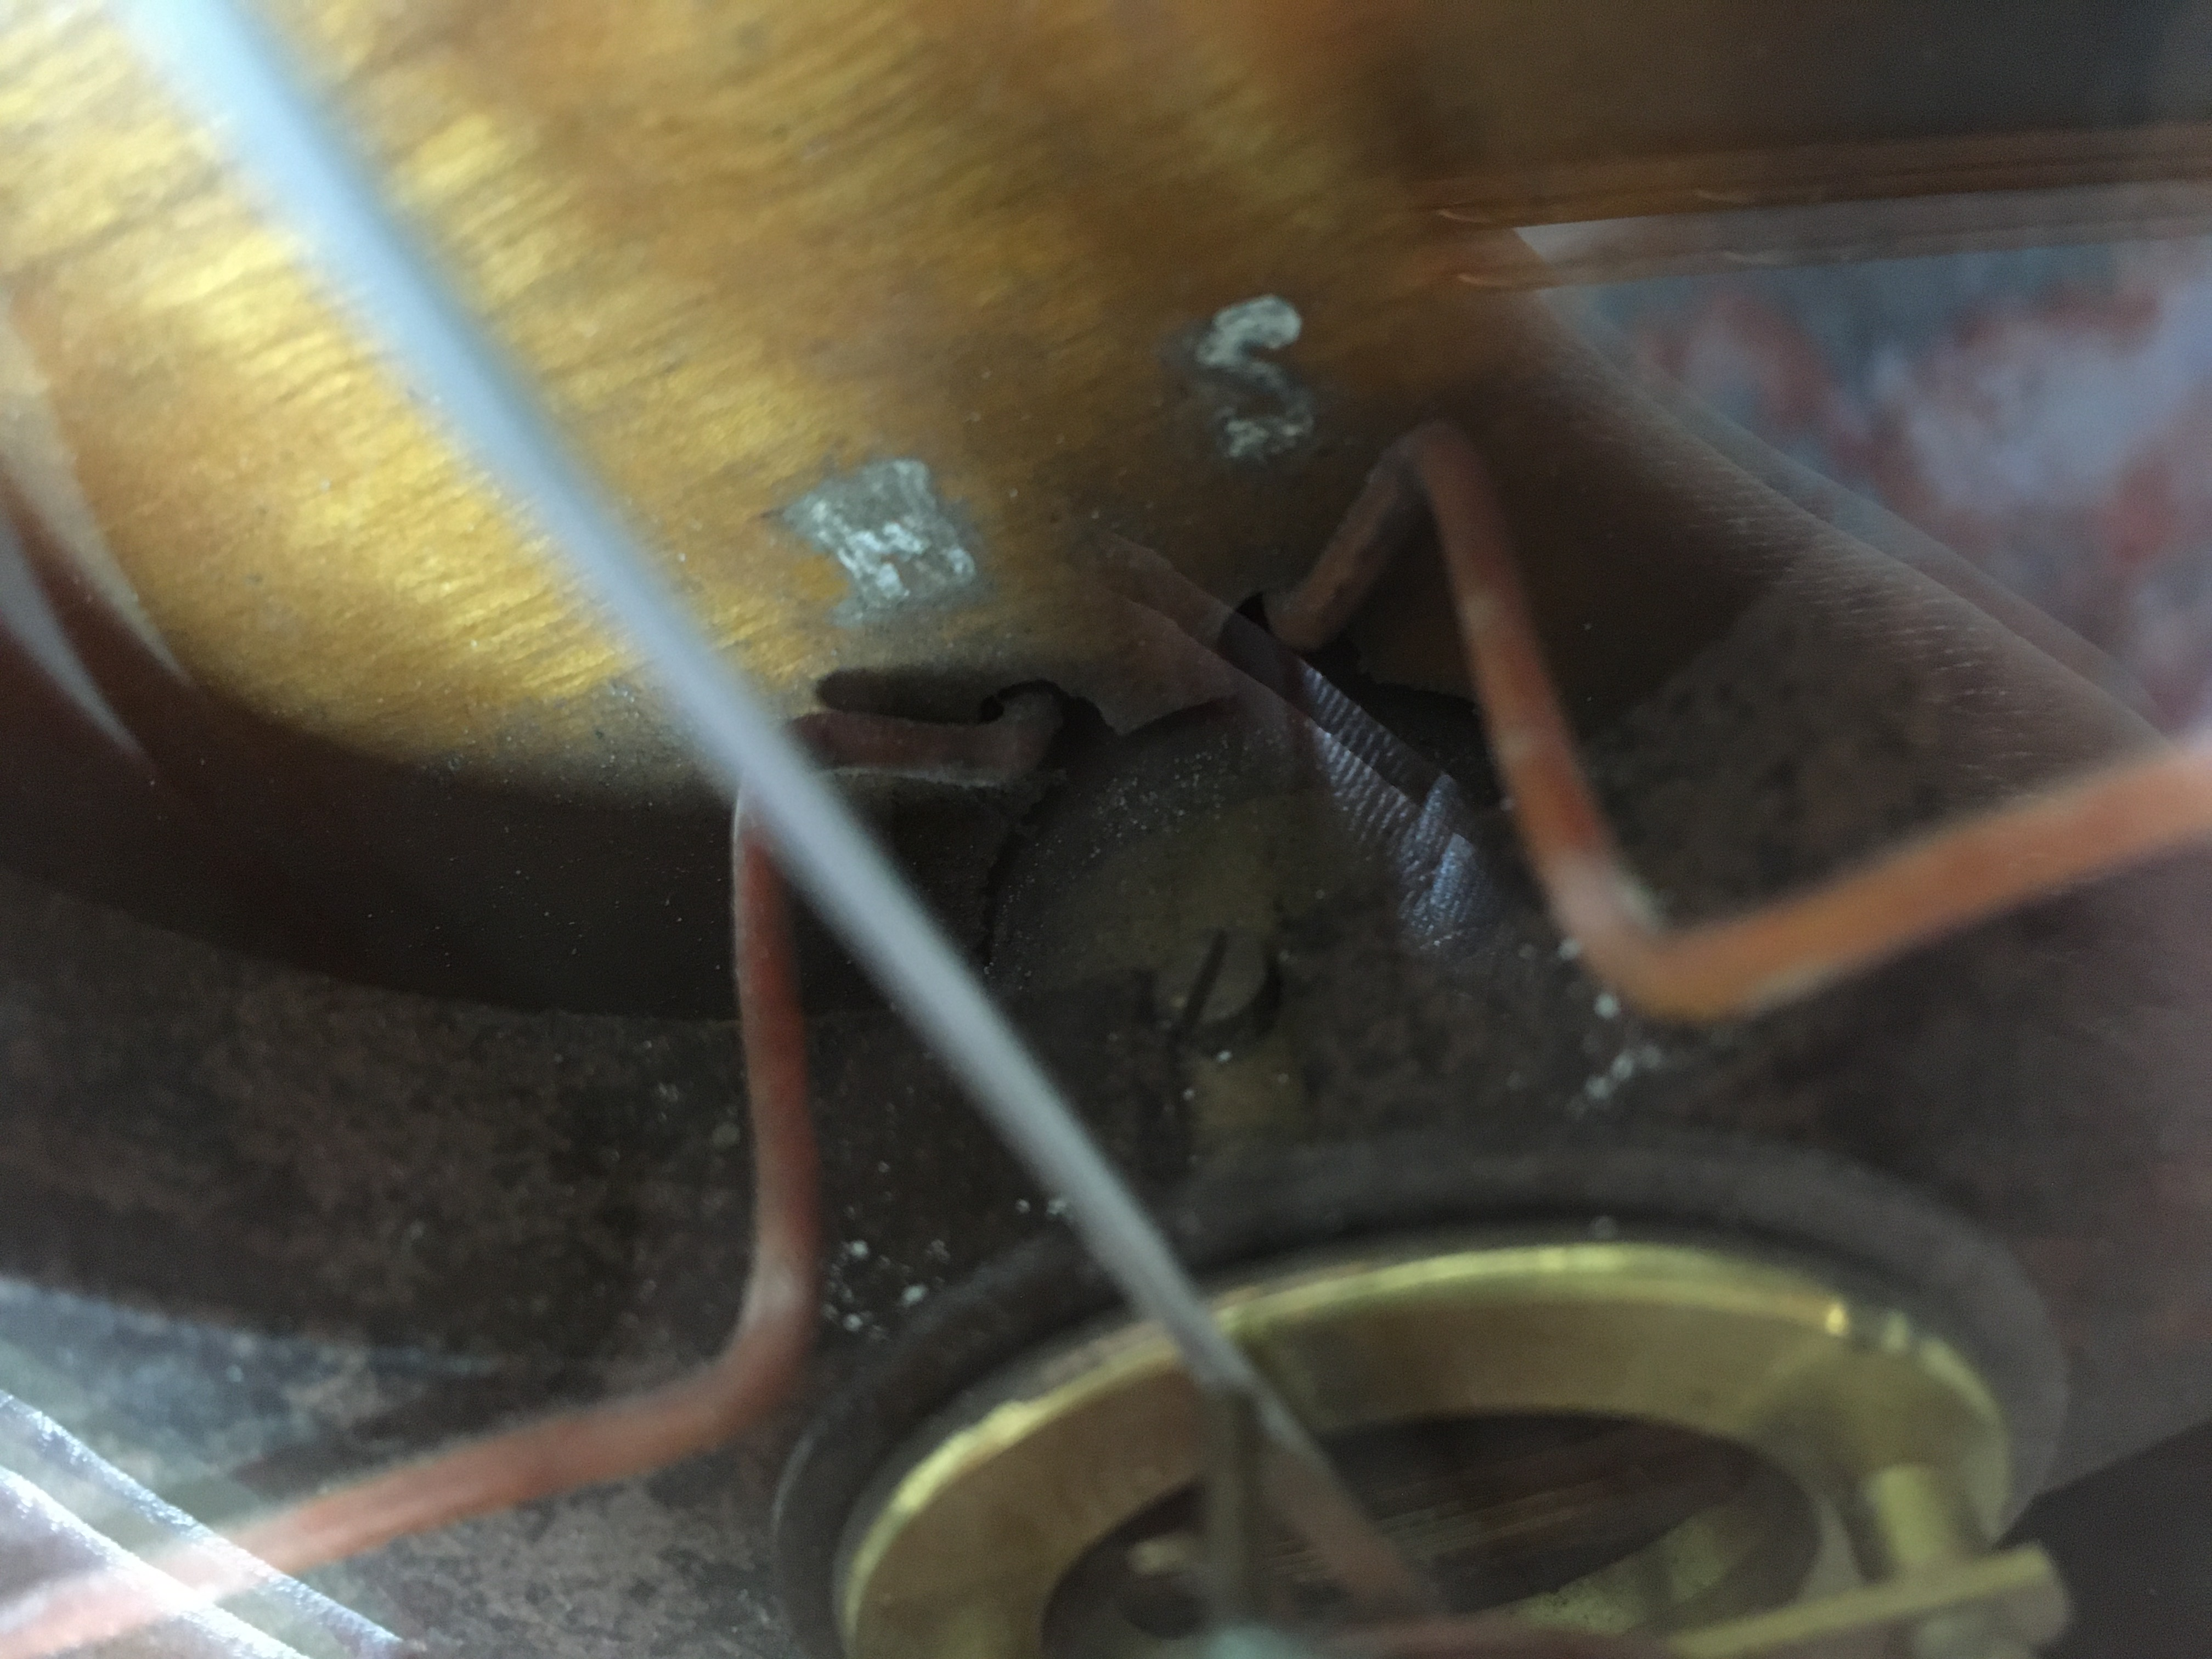
\includegraphics[width=\linewidth, trim=0 0 0 1000, clip, angle=180]{images/IMG_4050.jpg}
    \caption{L'entrefer de l'aimant permanent est à l'évidence de forme concave.
    On devine également la présence d'un bloc autour duquel pivote le cadre mobile.}
    \label{fig:theproof}
\end{figure}

\subsection{Remarques sur la conception des appareils}

La présence de frottements lors des mouvement du cadre mobile est essentielle au bon fonctionnement de l'appareil : ils permettent de s'assurer que l'aiguille atteigne sa position d'équilibre \og sans oscillations et néanmoins avec exactitude \fg{} (Ann.~\ref{ann:catalogue}).
Les appareils étudiés sont \emph{apériodiques}, ce qui semble faire référence à cette absence d'oscillations lors du régime transitoire : on pourrait ainsi contraindre la valeur de $\alpha$ dans notre modèle.

La longévité de la calibration des instruments repose notamment sur la constance du champ magnétique produit par l'aimant permanent.
Dans le catalogue constructeur (Ann.~\ref{ann:catalogue}), on peut également lire que le principe de fonctionnement de ces instruments \og \emph{permet de réaliser des appareils de mesure dont la permanence de l'étalonnage peut-être considérée comme pratiquement absolu} \fg{}.
Derrière cet argument de vente percutant se cachent deux vérités :
\begin{itemize}
\item \og la très faible force magnétomotrice développée par le courant traversant les spires du cadre mobile et qui est sans action appréciable sur l'aimant permanent \fg{} ;
\item la forme torique de l'aimant conduit naturellement à des lignes de champs quasiment fermées, ce qui préserve l'aimantation de l'aimant.
\end{itemize}

\section{L'ampèremètre}

\begin{figure}[htbp]
    \center
    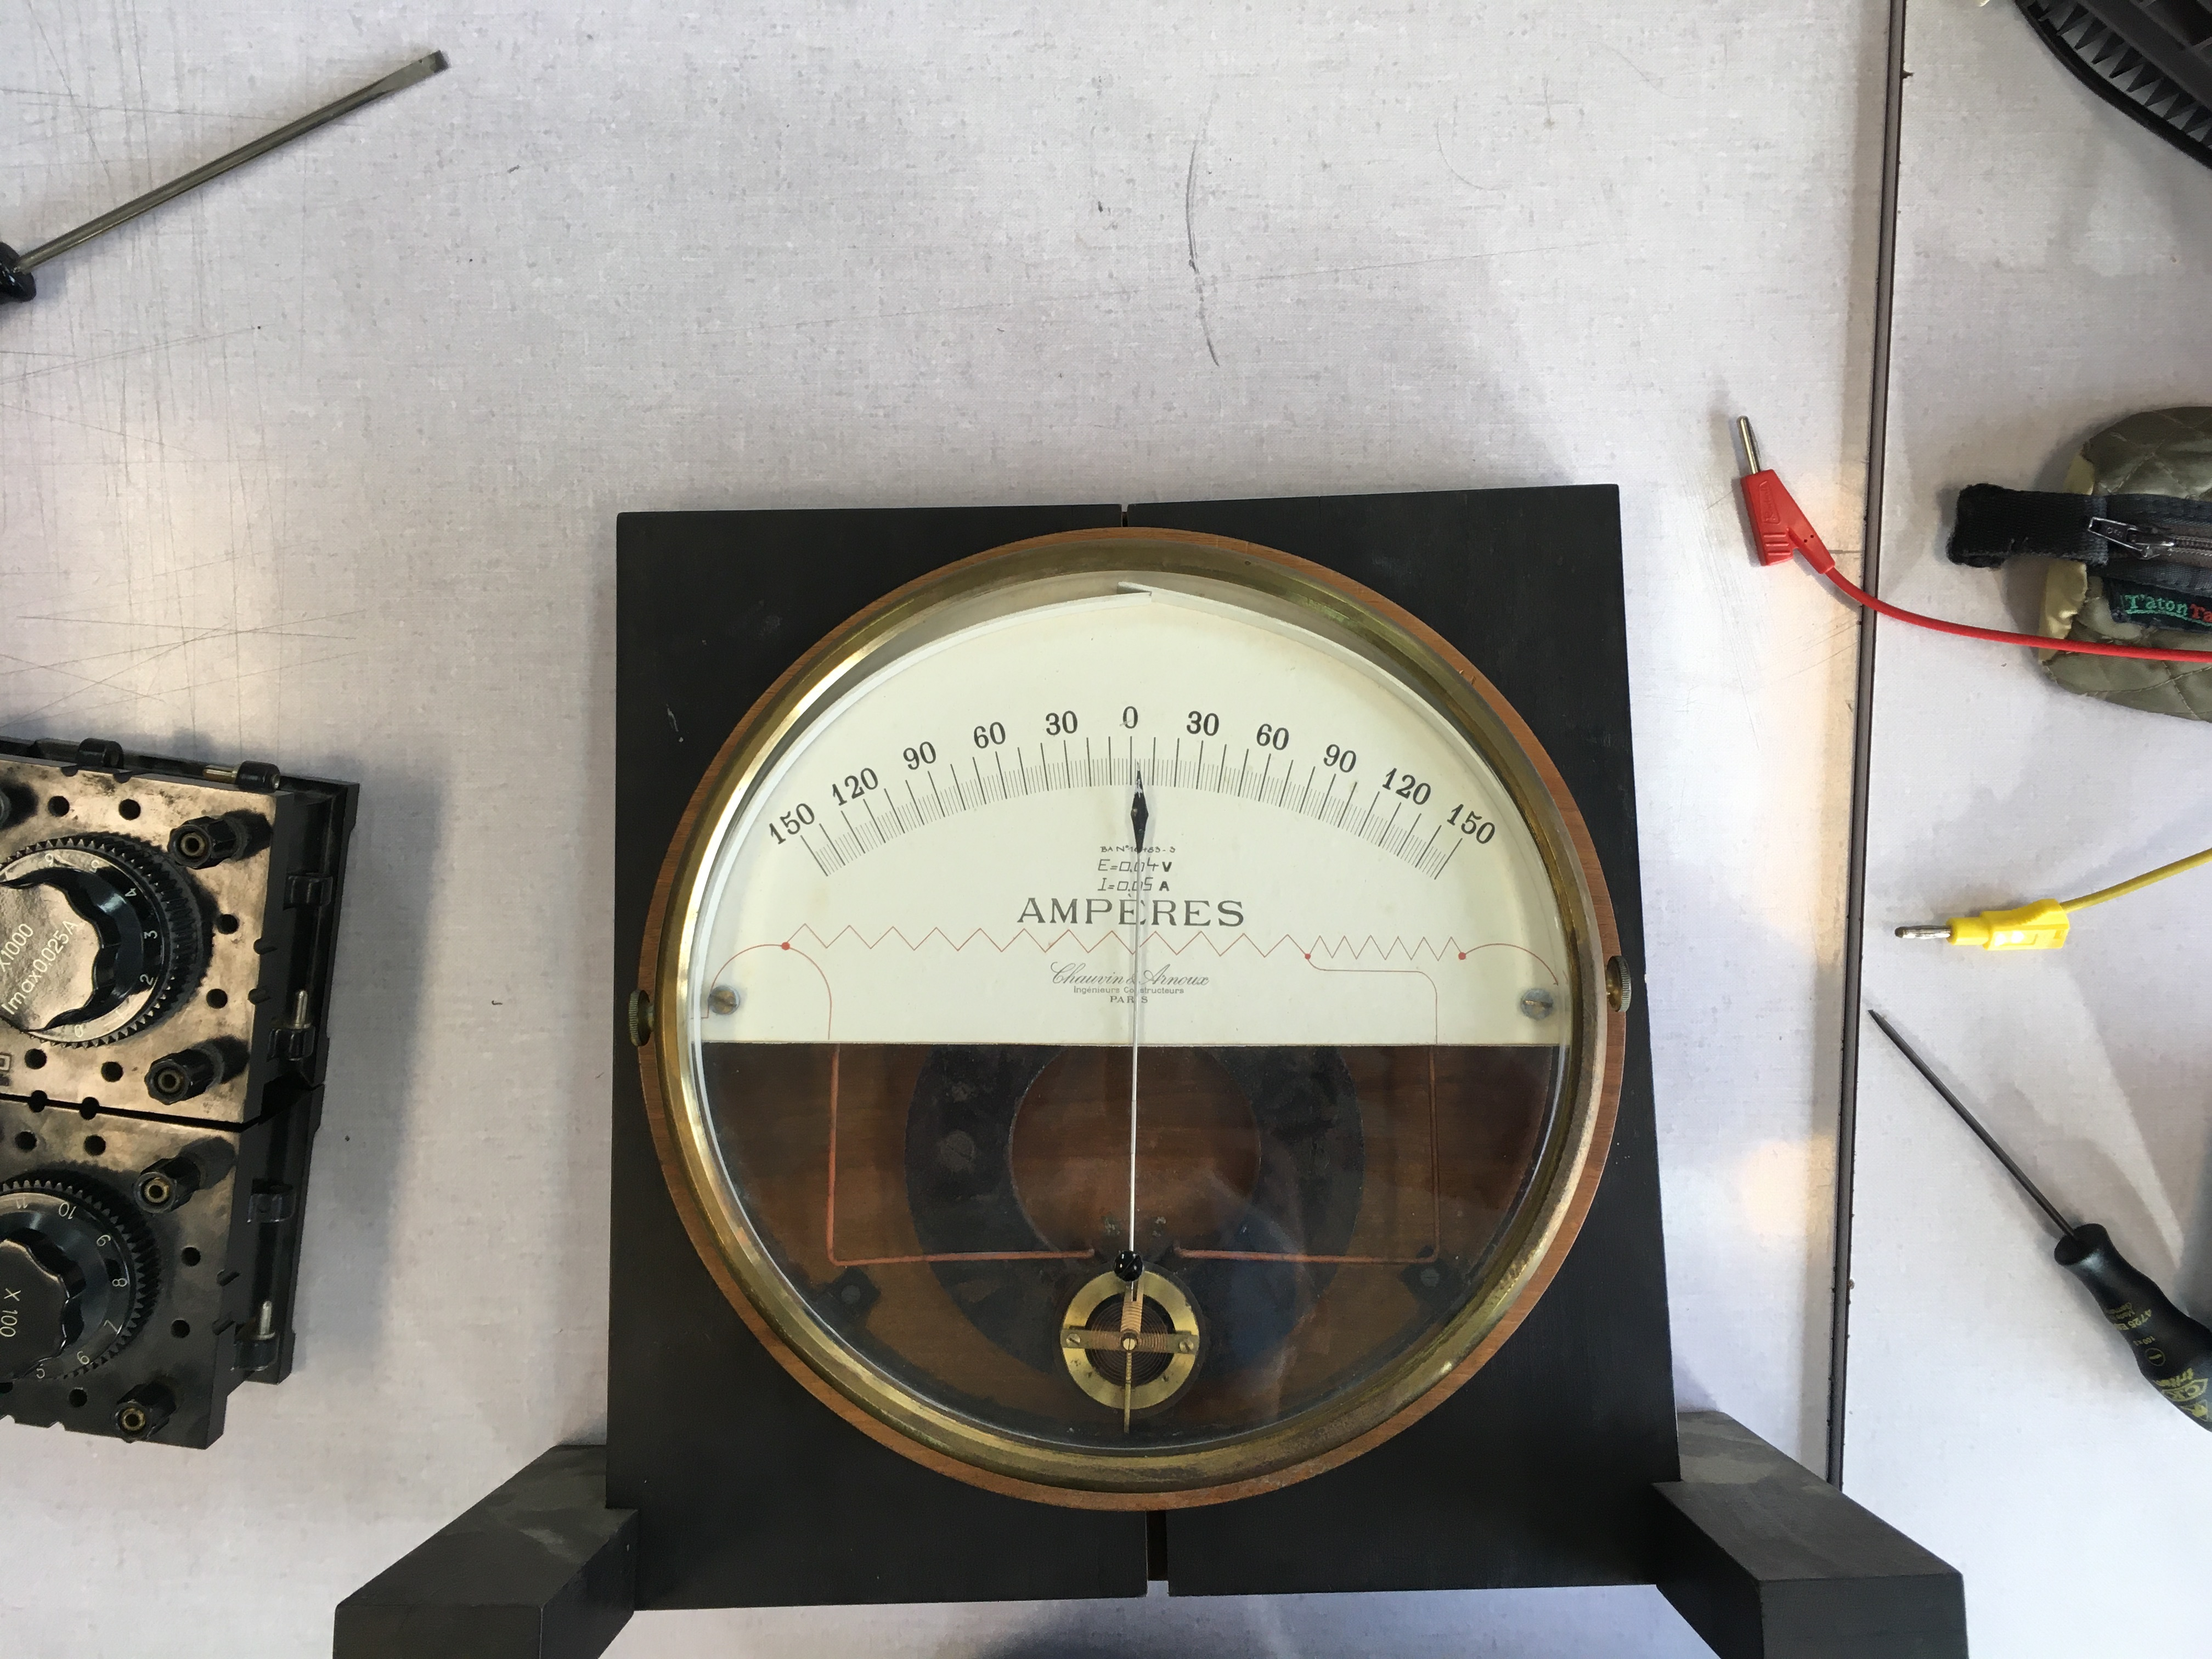
\includegraphics[height=300 pt, trim=800 0 700 800, clip]{images/IMG_4012.JPG}
    \caption{Le galvanomètre ampèremètre avant toute manipulation.}
    \label{fig:galva_amp_av}
\end{figure}

L'ampèremètre auquel on s'intéresse ici était commercialisé par Chauvin \& Arnoux, probablement au cours de la première moitié du XX\textsuperscript{ème} siècle.
Il s'agit d'un modèle de \SI{25}{cm} de diamètre, qui peut fonctionner quelque soit le sens du courant (continu) et dont le cadran possède 150 graduations dans chaque sens.
Bien que ce modèle précis ne soit pas dans le catalogue du fabricant présenté en annexe (Ann.~\ref{ann:catalogue}), on en trouve un modèle très similaire, qui était vendu au prix de 130 francs en 1915, soit environ 360 euros actuels \cite{Alexandre2014}.
Le galvanomètre est monté sur un support en bois qui le maintient à la verticale.

Quand on le récupère sur son étagère pour l'examiner, le galvanomètre est en bon état et à peine poussiéreux.
Comme premier test, on mesure sa résistance interne à l'aide d'un multimètre numérique : la résistance lue est de l'ordre de \SI{1}{\ohm}, trop faible pour être mesurée précisément avec cet appareil.
De plus lorsque le multimètre est connecté aux bornes du galvanomètre, l'aiguille de ce dernier bouge de quelques graduations : il semble donc en état de marche.
Il y a toutefois quelques problèmes mineurs :
\begin{itemize}
    \item en l'absence de courant, l'aiguille n'est pas centrée en zéro, et le réglage de l'\og offset \fg{} est en bout de course ;
    \item le système de graduation est mystérieux ;
    \item l'aiguille et notamment sa pointe sont légèrement tordues.
\end{itemize}
Une expérience rapide permet de s'assurer qu'il permet de réaliser des mesures (Fig.~\ref{fig:galva_amp_mes}).

\begin{figure}[htbp]
    \center
    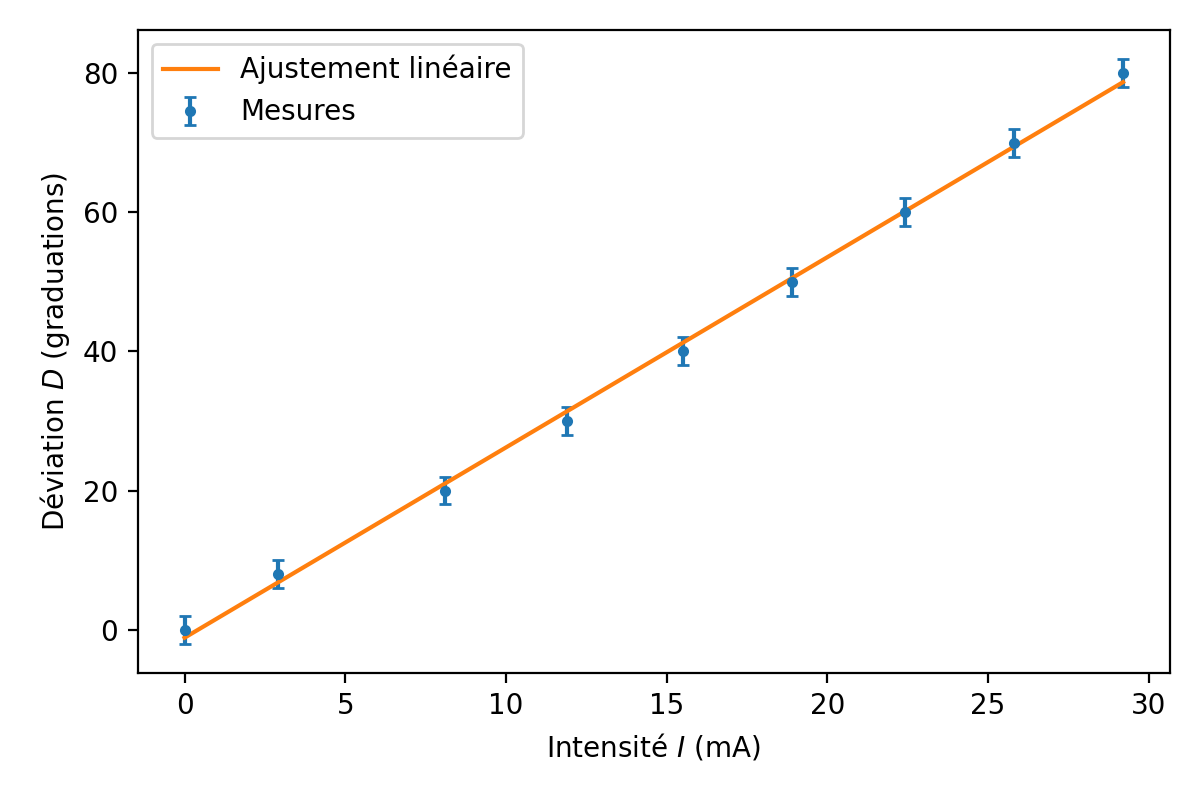
\includegraphics[scale=1]{images/mesure.png}
    \caption{Vérification du fonctionnement de l'instrument du galvanomètre ampèremètre.
    Le circuit utilisé est une simple résistance de \SI{1}{\kilo\ohm} branchée à la sortie d'une alimentation variable stabilisée en tension.
    Le galvanomètre et un multimètre numérique utilisé comme ampèremètre sont branchés en série avec la résistance.
    On fait varier la tension de l'alimentation pour obtenir la courbe ci-dessus.
    Les barres verticales correspondent aux incertitudes de mesure avec le galvanomètre, correspondant à une graduation.}
    \label{fig:galva_amp_mes}
\end{figure}

En supposant que le galvanomètre fonctionne toujours comme en sortie d'usine, cette série de mesure permet de comprendre l'échelle de graduation.
Le coefficient directeur de la droite obtenu lors de l'ajustement des mesures donne \SI{2.74(7)}{graduation\per\milli\ampere}.
On compare aux valeurs indiqués sur le cadran : comme le suggère la notice, si la graduation la plus élevée (150) correspond au courant maximal mesurable avec l'instrument ($I_\mathrm{max}=\SI{0.05}{\ampere}$), le coefficient directeur devrait être de \SI{3}{graduation\per\milli\ampere}.
Ces deux valeurs sont raisonnablement proches à ce stade pour supposer que la dernière graduation correspond à la valeur maximale indiquée sur le cadran.
\footnote{La graduation du cadran en 150 divisions semble être commune à de nombreux modèles commercialisés par Chauvin \& Arnoux, même s'ils proposent d'autres échelles : 100, 125 et 150 divisions.}
On détermine donc la valeur du courant en effectuant un simple produit en croix.

Pour en apprendre davantage sur l'instrument, nous décidons de le démonter :
\begin{itemize}
    \item on l'enlève de son support vertical en bois en dévissant les quatre vis qui l'y maintiennent ;
    \item on retire la vitre de protection, maintenue par une bague en laiton ajustée au cylindre qui fait le tour de l'instrument.
    Pour cela, on procède avec précaution, en exerçant à l'aide d'un gros tournevis un effort sur le dessous de la bague pour la soulever, en prenant appui sur les bornes de branchement de l'instrument pour faire un levier.
    La vitre repose simplement sur deux grands anneaux, l'un métallique et l'autre cartonné ;
    \item on retire le cadran en dévissant les deux vis en laiton, puis en le faisant pivoter à droite, tout en maintenant l'aiguille complètement à gauche.
\end{itemize}
On se retrouve alors avec l'intérieur de l'instrument mieux visible (Fig.~\ref{fig:galva_amp_int}).

\begin{figure}[htbp]
    \center
    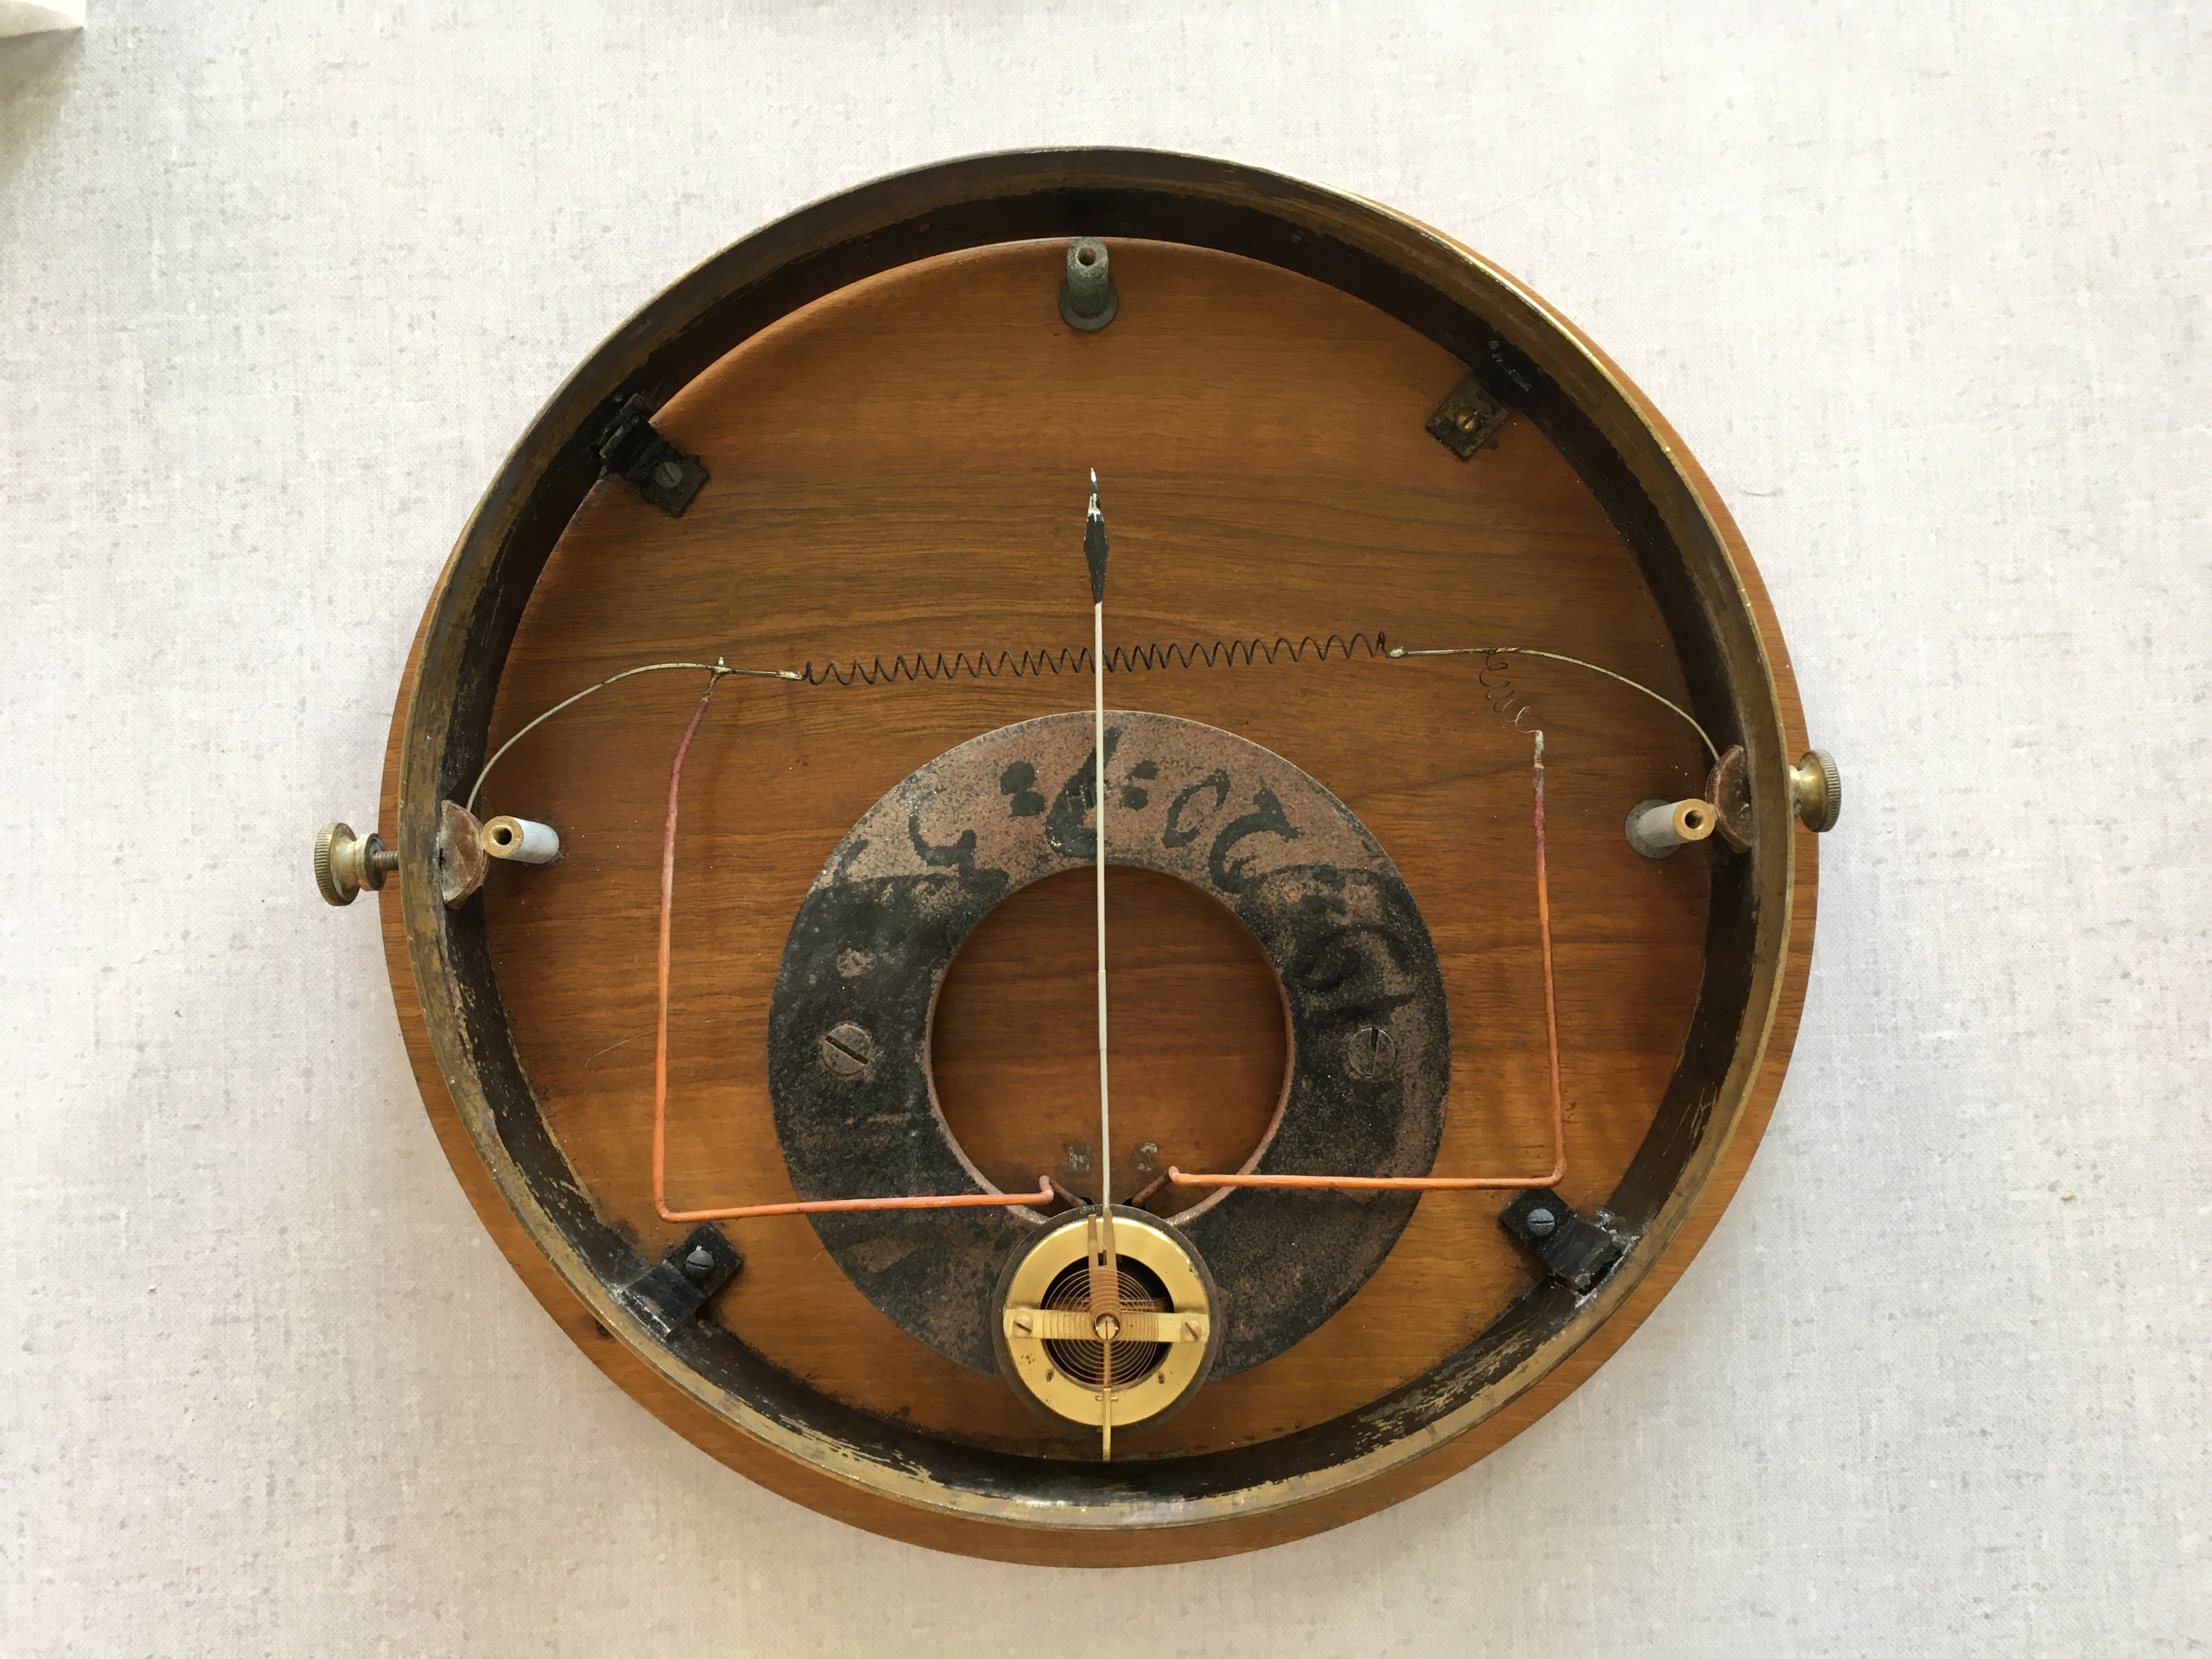
\includegraphics[height=300 pt, trim=500 100 600 200, clip]{images/IMG_4037.JPG}
    \caption{Le même galvanomètre, une fois la vitre et le cadran retirés.}
    \label{fig:galva_amp_int}
\end{figure}

En plus des fils qui alimentent le cadre mobile, on remarque la présence d'un fil en forme de ressort qui relie les bornes du galvanomètre.
Dans la notice (Ann.~\ref{ann:catalogue}), il est indiqué que la bobine du cadre mobile est de l'ordre de \SI{0.5}{\ohm}.
Il est par ailleurs indiqué qu'\og une résistance en métal à coefficient de température nul est ajoutée pour le tarage de l'appareil \fg{}.
Il semblerait que ce soit cette résistance qui fixe le calibre de l'appareil : plus la résistance est faible, plus il sera possible de mesurer des courants intenses puisque la plupart du courant passera à travers cette résistance.
On parle de \emph{shunt}.
Les indications du cadran ($I_\mathrm{max}=\SI{0.05}{A}$ et $U_\mathrm{max}=\SI{0.04}{V}$) permettent de déduire la résistance équivalente de l'ensemble, correspondant à la résistance interne de l'appareil : on trouve \SI{0.8}{\ohm}.
Cette résistance est difficilement vérifiable en raison de sa faible valeur.

Alors que nous reprenons le galvanomètre pour effectuer des tests, nous nous apercevons que l'aiguille ne bouge plus lorsque l'appareil est branché dans un circuit.
La mesure de la résistance interne totale de l'appareil entre ses deux bornes montre pourtant que le circuit est fermé, que les deux bornes sont bien reliées électriquement.
Avec un montage réalisé trop rapidement, nous apercevons de la fumée qui s'échappe de l'appareil : nous débranchons immédiatement le tout.
\footnote{La fumée qui s'est échappée de l'appareil provient du matériau isolant qui recouvre le \emph{shunt}.
Celui-ci a trop chauffé pendant cette manipulation maladroite, sans toutefois dégrader le fonctionnement de l'appareil.}
Il apparait donc qu'un courant parcours l'appareil, mais comme l'aiguille ne réagit pas, nous suspectons un problème de connection entre le \emph{shunt} et la bobine du cadre mobile.

Une inspection plus poussée de l'appareil montre en effet qu'une des brasures situées à l'arrière de l'appareil, qui relie une borne de la bobine du cadre mobile à l'un des fils gainés oranges est cassée.
Après avoir gratté la peinture noire qui recouvre l'étain sur la brasure, nous la consolidons avec un apport d'étain supplémentaire.
L'appareil est à nouveau en bon état de marche.

L'instrument est finalement remonté après avoir nettoyé chaque pièce et notamment la vitre de protection, en veillant particulièrement à deux points :
\begin{itemize}
\item l'aiguille doit être parfaitement droite pour évoluer librement dans l'espace réduit entre la vitre et le cadran ;
\item le réglage du zéro doit permettre de placer l'aiguille au centre du cadran : on y parvient en décalant légèrement la vitre pour placer convenablement le dispositif de réglage (voir section~\ref{sec:remontage_volt} pour plus de détails : les deux appareils étudiés sont conçus de manière très similaire).
\end{itemize}
Le travail de restauration sur cet appareil est donc assez limité puisque celui-ci était déjà en état de marche.
Son démontage nous a cependant permis de mieux comprendre le fonctionnement de ce type de galvanomètre.





\section{Le voltmètre}

Le galvanomètre utilisé comme voltmètre que nous avons choisi d'étudier pour ce rapport est un appareil commercialisé par la société Chauvin \& Arnoux, probablement du début du XX\textsuperscript{ème} siècle, au regard de la notice de 1915 (Ann.~~\ref{ann:catalogue}).

\subsection{Description de l'appareil}

Le voltmètre est composé d'un cadre en laiton de 25 cm de diamètre fixé sur une plaque de bois circulaire, elle-même fixée sur un support de bois (noir) permettant de maintenir l'appareil en position verticale.
L'aiguille est protégée par une plaque de verre circulaire qui comporte un insert permettant d'ajuster la position de l'aiguille sur le zéro de la graduation.
L'aiguille est mobile, quand nous déplaçons l'appareil elle oscille légèrement et semble en bon état, le réglage du zéro est encore possible (Fig.~\ref{fig:galva_volt_av}).
\begin{figure}[htbp]
    \center
    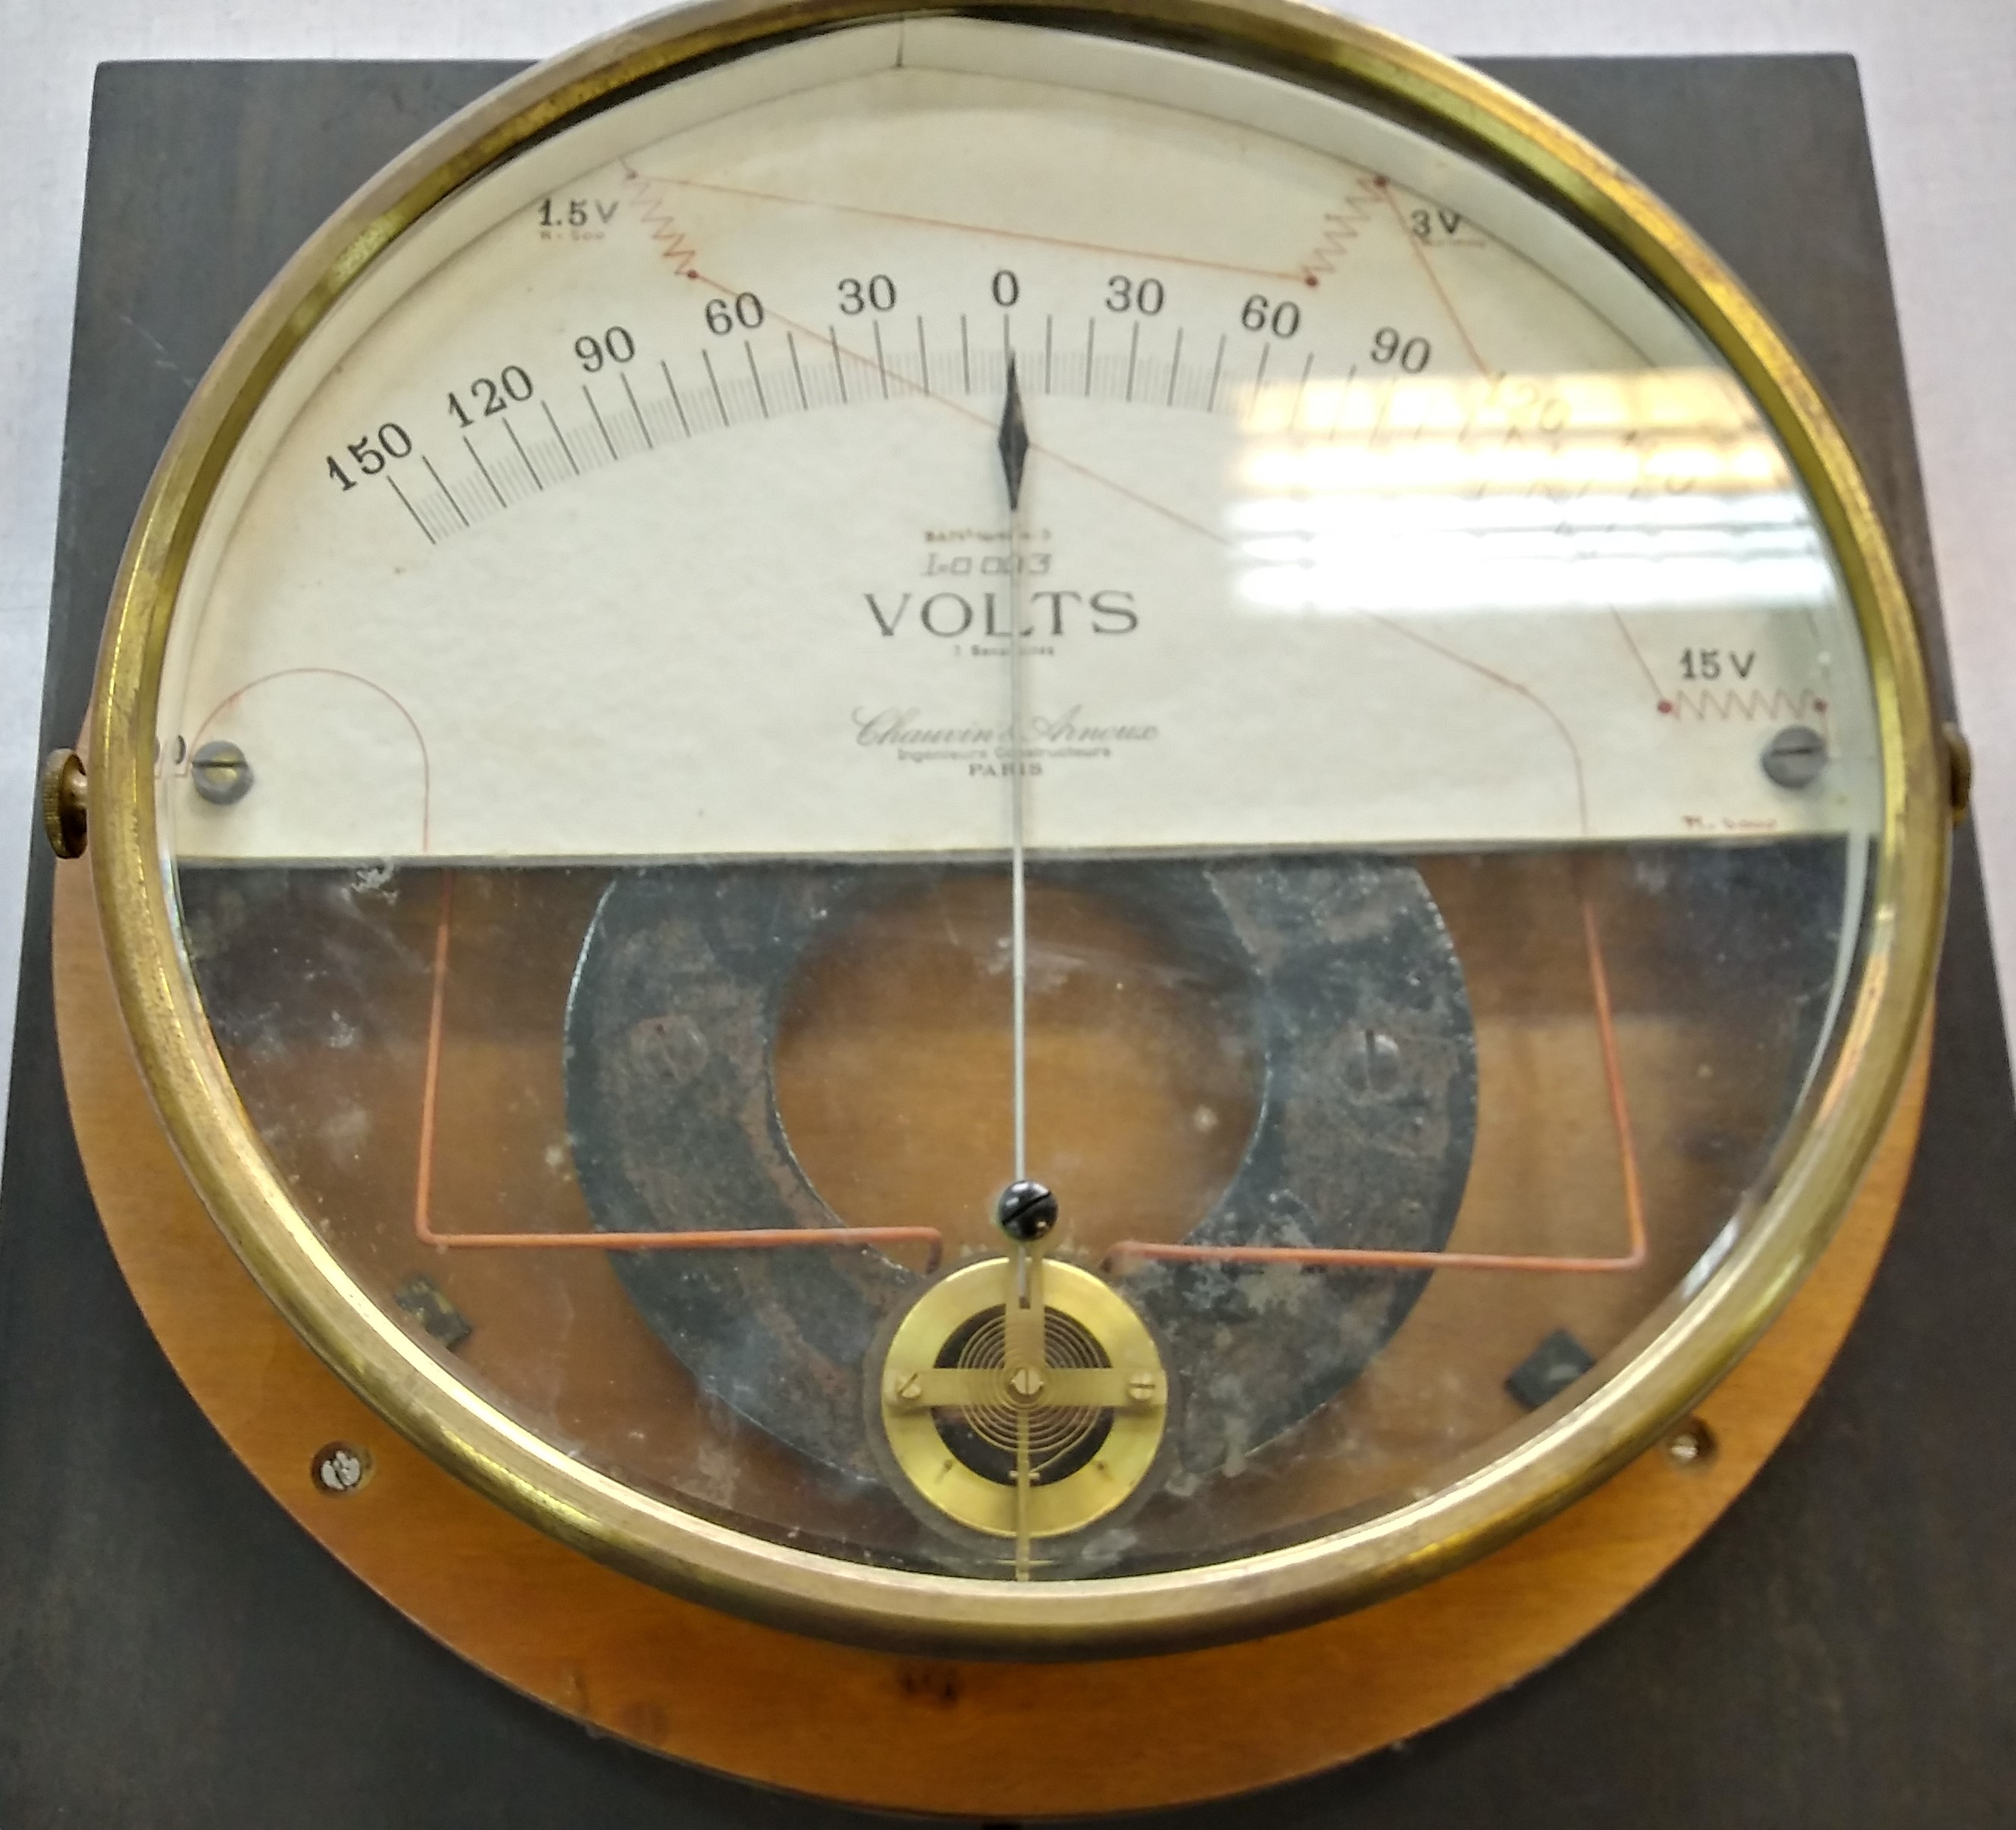
\includegraphics[height=300 pt]{images/20210205_150347_HDR.jpg}
    \caption{L'appareil avant le démontage.}
    \label{fig:galva_volt_av}
\end{figure}

Le cadran est gradué de 0 à 150 par pas de 2 dans les deux directions et semble destiné à mesurer les tensions des courants continus.
Cet appareil ressemble très fortement à la description de la notice du constructeur et nous pouvons estimer son prix de 1915 selon les caractéristiques disponibles à ce stade :
\begin{itemize}
\item 130 francs pour un appareil de diamètre \SI{25}{\centi\metre} ;
\item trois sensibilités en 150 divisions :
\begin{itemize}
\item \SI{15}{V} par \num{0.1} : 10 francs ;
\item \SI{3}{V} par \num{0.02} : 5 francs ;
\item \SI{1.5}{V} par \num{0.1} : 5 francs ;
\end{itemize}
\end{itemize}
pour une estimation à 150 francs de 1915,  soit un peu moins de 400 euros de 2021.
L'appareil comporte quatre \og bornes \fg{} sur la partie supérieure et une ligne rouge semble symboliser le circuit interne de l'appareil (Fig.~\ref{fig:galva_volt_glass}).
Il semble que pour une utilisation normale, le courant passe par la borne 0 (position Ouest) et par une des trois autres bornes (\SI{1.5}{V}, \SI{3}{V} et \SI{15}{V}) pour pouvoir traverser la bobine du cadre mobile.
Les bornes portent des valeurs qui font immédiatement penser à des calibres à la manière des voltmètres modernes.
\begin{figure}
    \center
    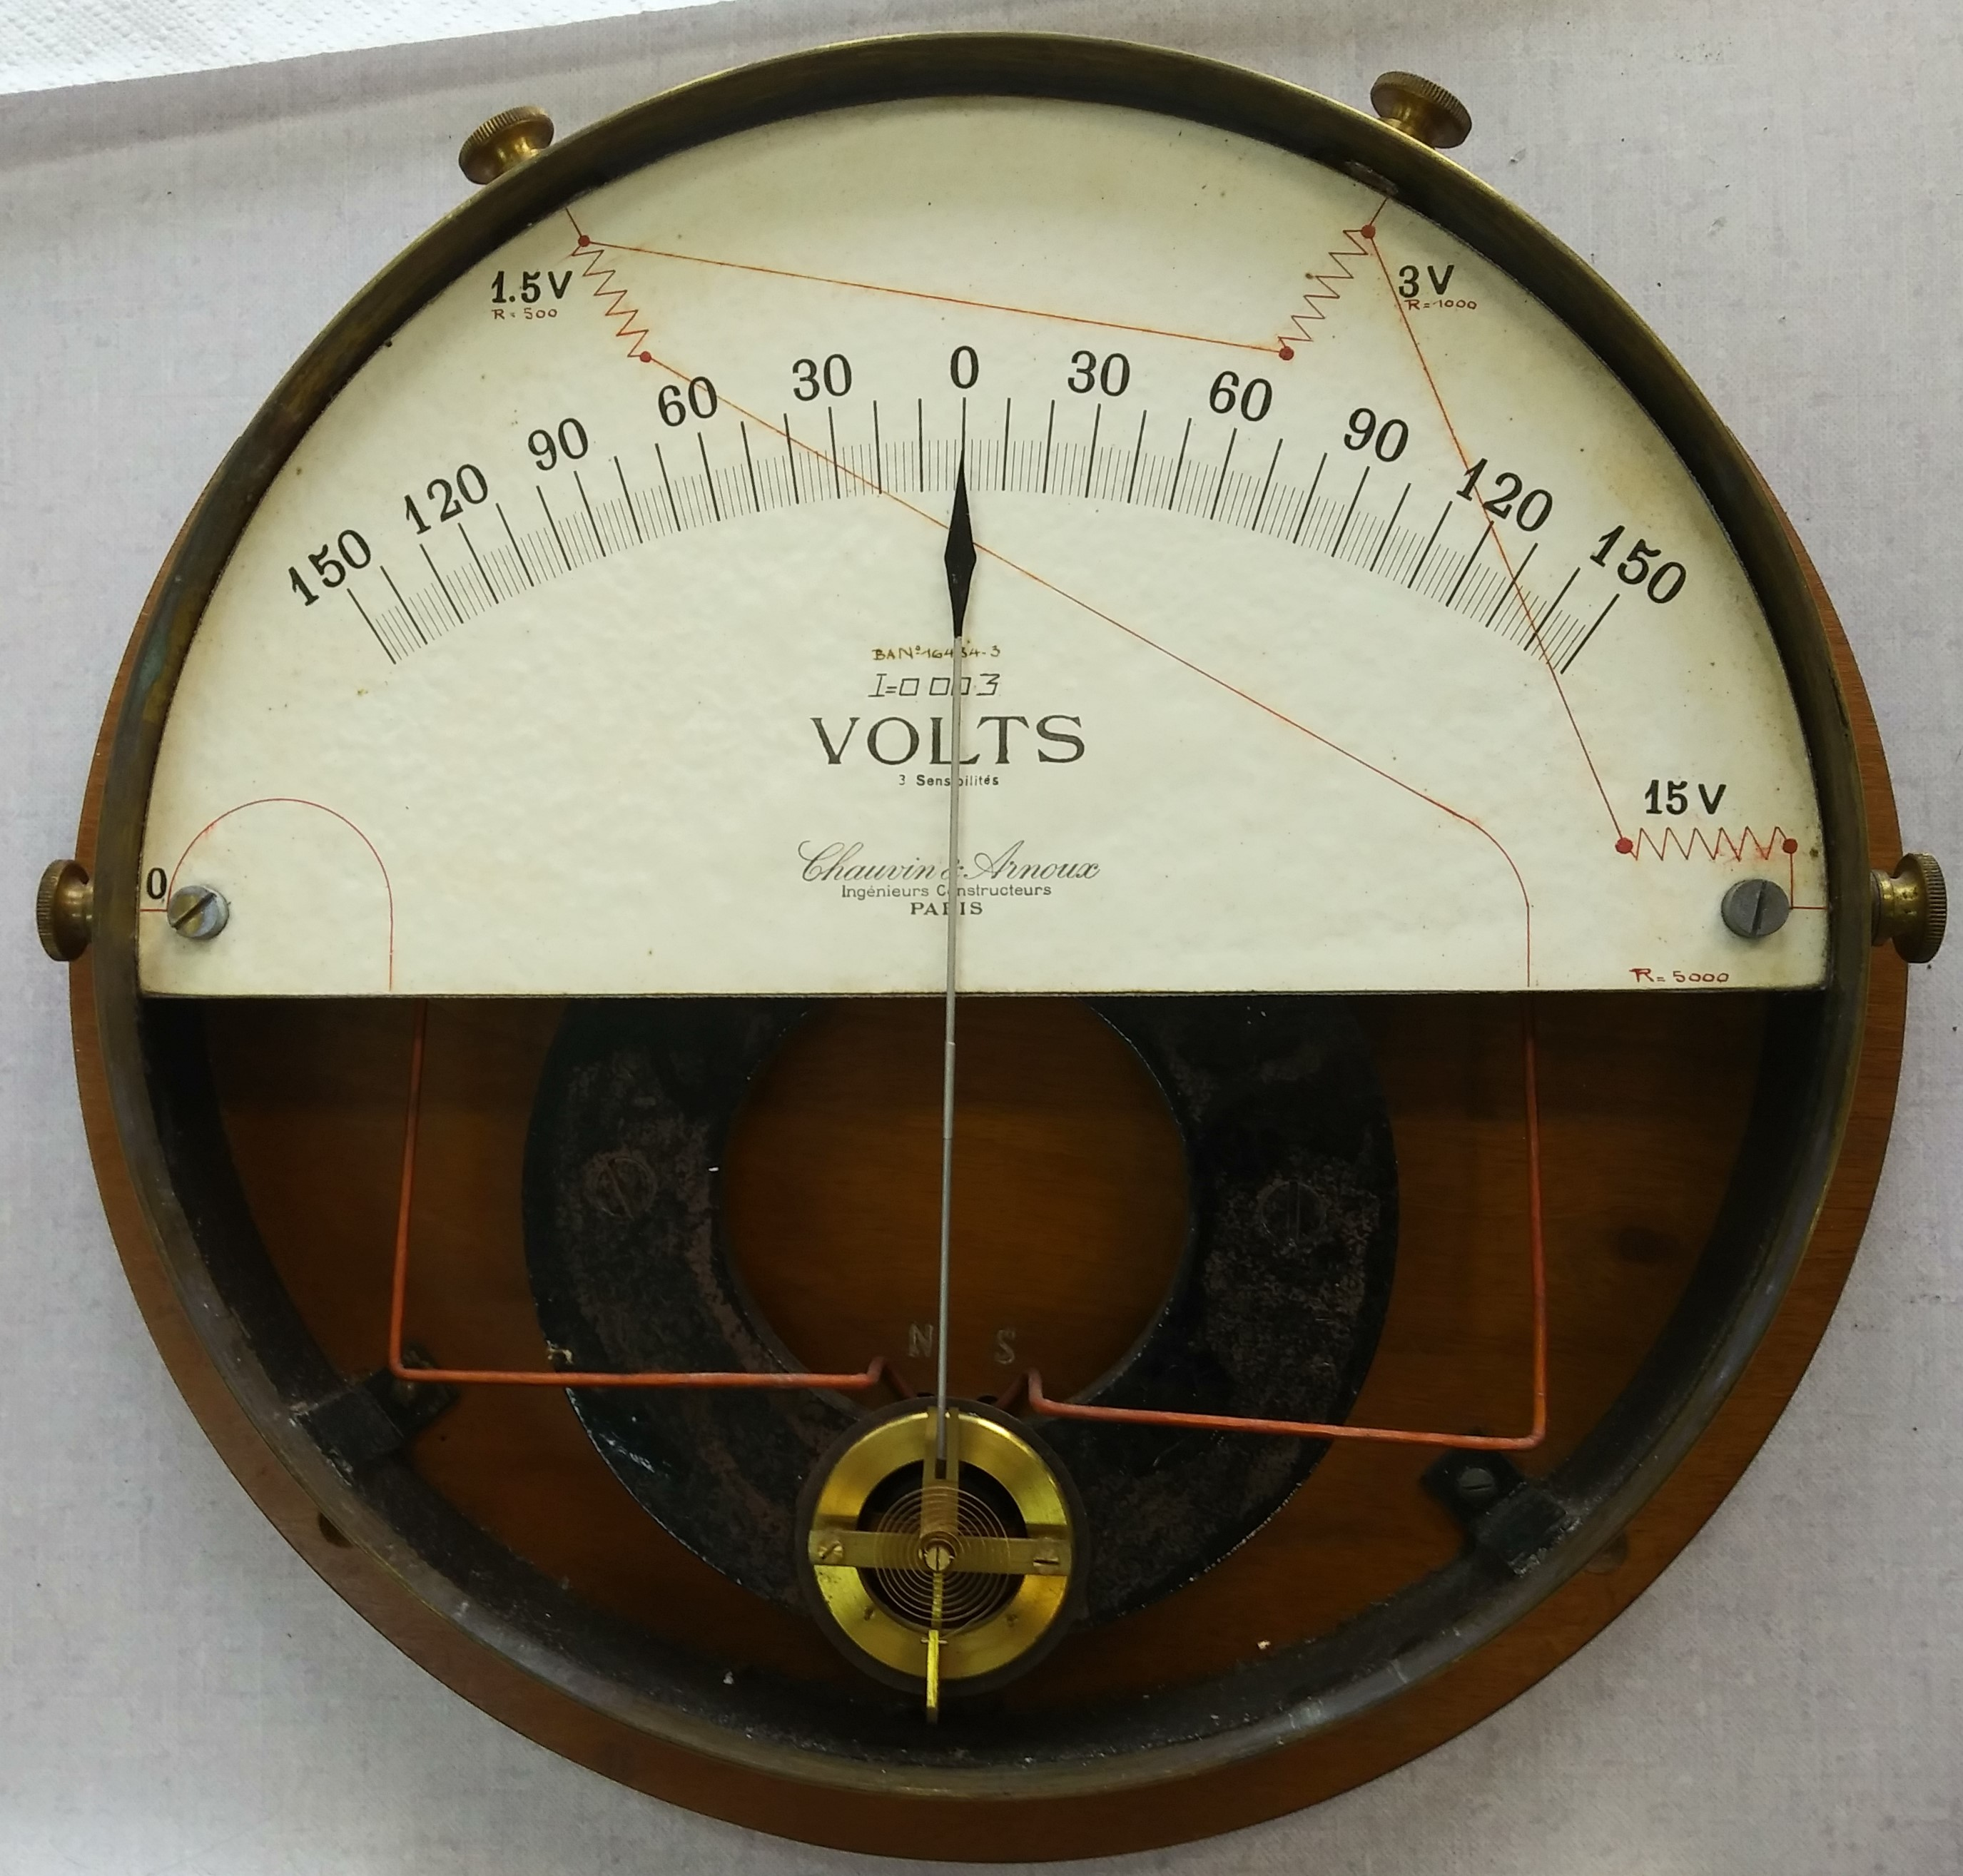
\includegraphics[height=300 pt]{images/20210205_152634.jpg}
    \caption{L'appareil après démontage de la vitre.}
    \label{fig:galva_volt_glass}
\end{figure}

La borne \SI{1.5}{V} (position Nord Nord Ouest) porte l'indication \og R = 500 \fg{} et le schéma électrique tracé en rouge semblent indiquer qu'un dipôle, probablement une résistance se situe au niveau de cette borne.

La borne \SI{3}{V} (position Nord Nord Est) porte l'indication \og R = 1000 \fg{} et le schéma électrique tracé en rouge semblent indiquer que le courant traverse deux résistances avant d'entrer dans la bobine du cadre mobile.

La borne \SI{15}{V} (position Est) porte l'indication \og R = 5000 \fg{} et le schéma électrique tracé en rouge semblent indiquer que le courant traverse trois résistances avant d'entrer dans la bobine du cadre mobile.

Sur le cadran figure aussi une valeur \og I = 0{,}003 \fg{} faisant penser à une valeur d'intensité électrique.
En appliquant la loi d'ohm à ces valeurs, le tout semble cohérent : en effet, par exemple avec le calibre le plus élevé, on a $ \SI{15}{V} = \SI{5000}{\ohm} \times \SI{0.003}{A}$.
Cette valeur est donc sûrement l'intensité maximale traversant l'appareil à sa valeur limite de \SI{15}{V}.

\subsection{Premières expériences}

Nous avons essayé de placer l'appareil dans un circuit aux bornes d'un générateur de tension, en délivrant une tension inférieure au calibre sélectionné.
À ce stade, aucune mesure n'est possible : l'aiguille ne bouge pas.
Comme le cadran semble indiquer des résistances, nous utilisons un ohmmètre pour vérifier ces valeurs en utilisant les bornes de l'appareil.
Aucune combinaison de borne, que ce soit entre la borne 0 et les autres ou entre les bornes \SI{1.5}{V}, \SI{3}{V}, \SI{15}{V} entre elles, ne permet une mesure.
Nous utilisons ensuite le multimètre en testeur électrique sans parvenir à trouver de connexions entre les bornes de l'appareil.
Problèmes identifiés à ce stade : le courant ne circule pas dans l'appareil en utilisant les bornes extérieures.

Nous décidons donc d'enlever le cadran de mesure pour accéder aux composants de l'appareil. Il suffit pour cela de dévisser les vis en laiton qui maintiennent le cadran, de pivoter l'aiguille d'un côté et le cadran de l'autre pour le faire sortir.
Nous voyons sur la figure~\ref{fig:galva_volt_bob} que le circuit est composé, comme le schéma du cadran le laissait penser, de trois bobines résistives sur des broches en cuivre, branchées en série.
Une bobine résistive s'ajoute à la précédente quand le calibre de mesure augmente : une bobine résistive pour le calibre \SI{1.5}{V}, deux bobines résistives pour \SI{3}{V} et trois bobines résistives pour \SI{15}{V}.

\begin{figure}[htbp]
    \center
    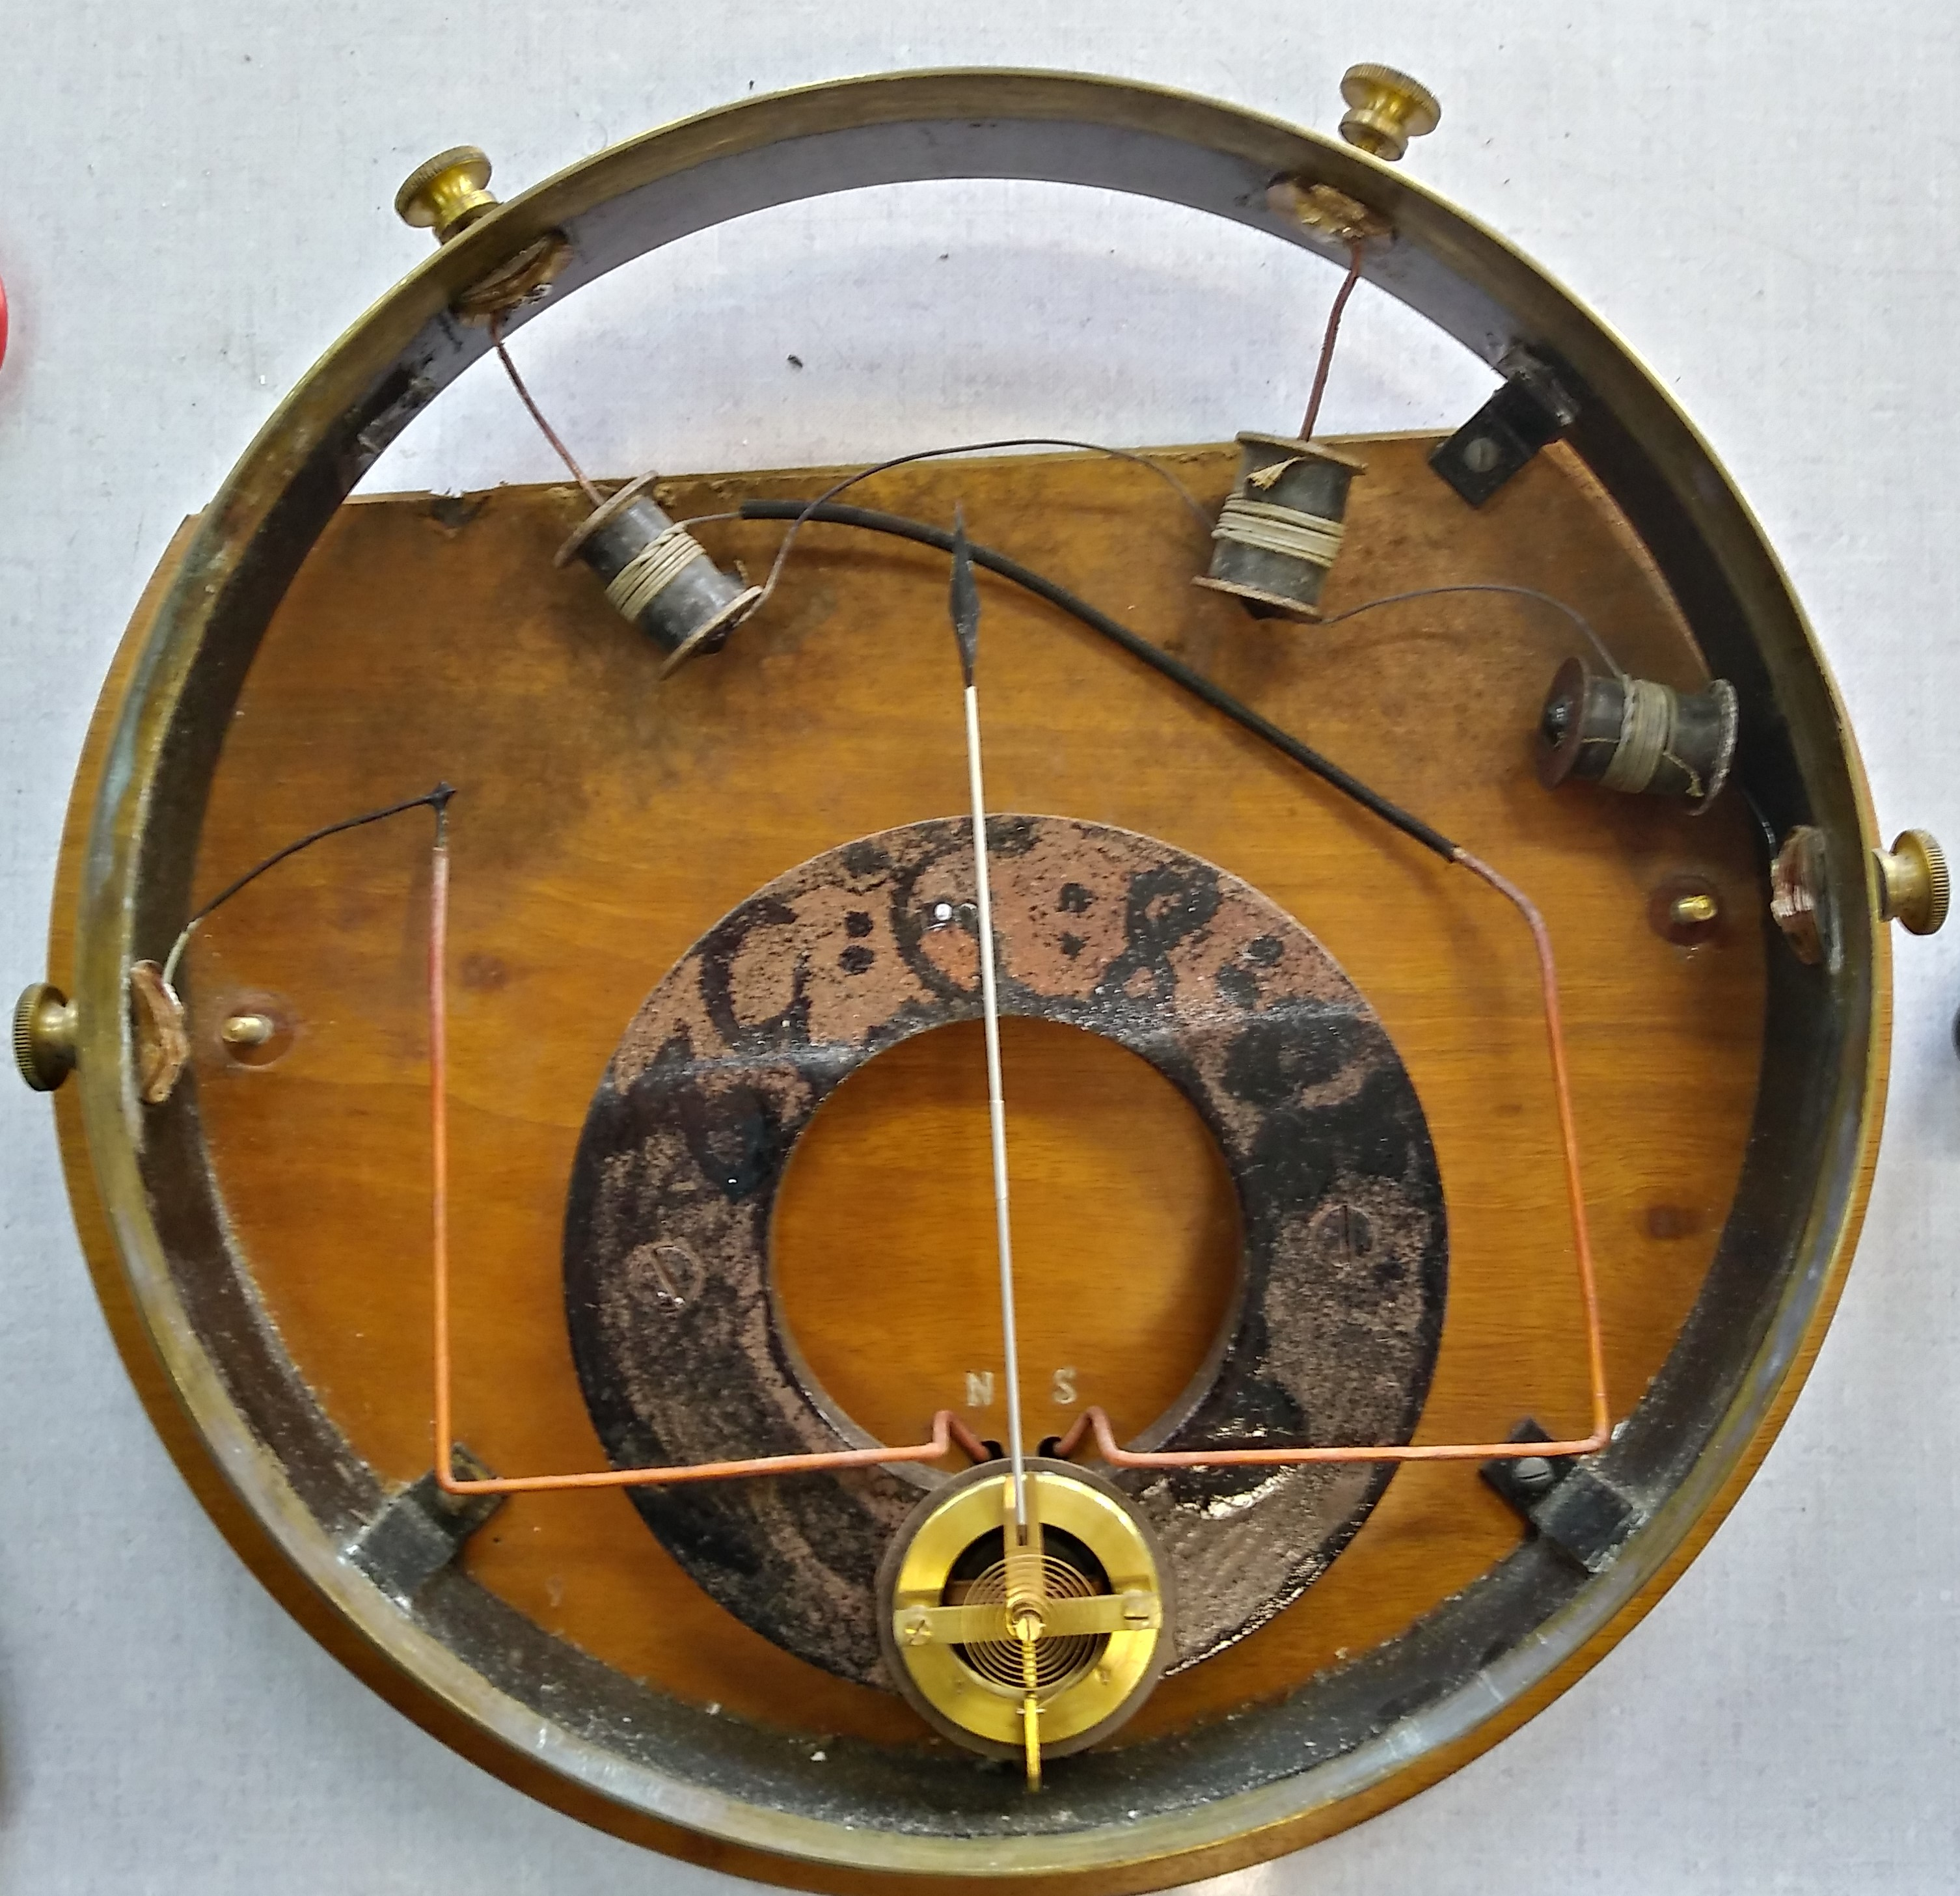
\includegraphics[height=300 pt]{images/20210205_155230_HDR.jpg}
    \caption{Une fois le cadran retiré, on remarque trois bobines résistives (numérotées pour la suite 1, 2 et 3, de gauche à droite).}
    \label{fig:galva_volt_bob}    
\end{figure}

Nous essayons de trouver un contact électrique avec le multimètre en grattant un peu le verni sur les soudures de part et d'autre des bobines résistives, sans succès.
Nous réussissons cependant à faire bouger légèrement l'aiguille en appliquant un courant faible (courant de test de conductivité du multimètre) à la bobine seule en créant un contact électrique directement au niveau des soudures des fils gainés oranges.
Hypothèse à ce stade : le fil d'une ou plusieurs bobines est cassé ou trop endommagé pour conduire le courant, mais la bobine sur le cadre mobile à l'intérieur de l'aimant fonctionne toujours.
Nous décidons de démonter les bobines résistives une à une en commençant par la plus proche de la bobine du cadre mobile (Fig.~\ref{fig:bobine}).
En espérant qu'une seule des trois soit défectueuse.

\subsection{Les bobines résistives}

\subsubsection{Démontage des bobines}

\paragraph{Protocole pour le démontage et la caractérisation des bobines :}
\begin{itemize}
\item la bobine est dessoudée de la borne de l'appareil.
La brasure d'origine semble faite avec de l'étain : en effet le métal fond grâce à un fer à souder réglé sur \qty{400}{\degreeCelsius} ;
\item la broche de cuivre traverse l'axe de la bobine et les deux pièces sont maintenues par une brasure à l'étain du côté opposé de la borne de l'appareil.
On la retire également avec le fer à souder ;
\item le diamètre du fil résistif est mesuré grâce à un pied à coulisse, puis avec un micromètre ;
\item la bobine est ensuite déroulée dans un long couloir et la longueur de fil mesurée grâce à un décamètre ;
\item la résistivité du fil a été mesurée avec un ohmmètre sur la plus grande distance possible de fil intacte, dont la longueur est mesurée grâce à un décamètre.
\end{itemize}

\begin{figure}[htbp]
    \center
    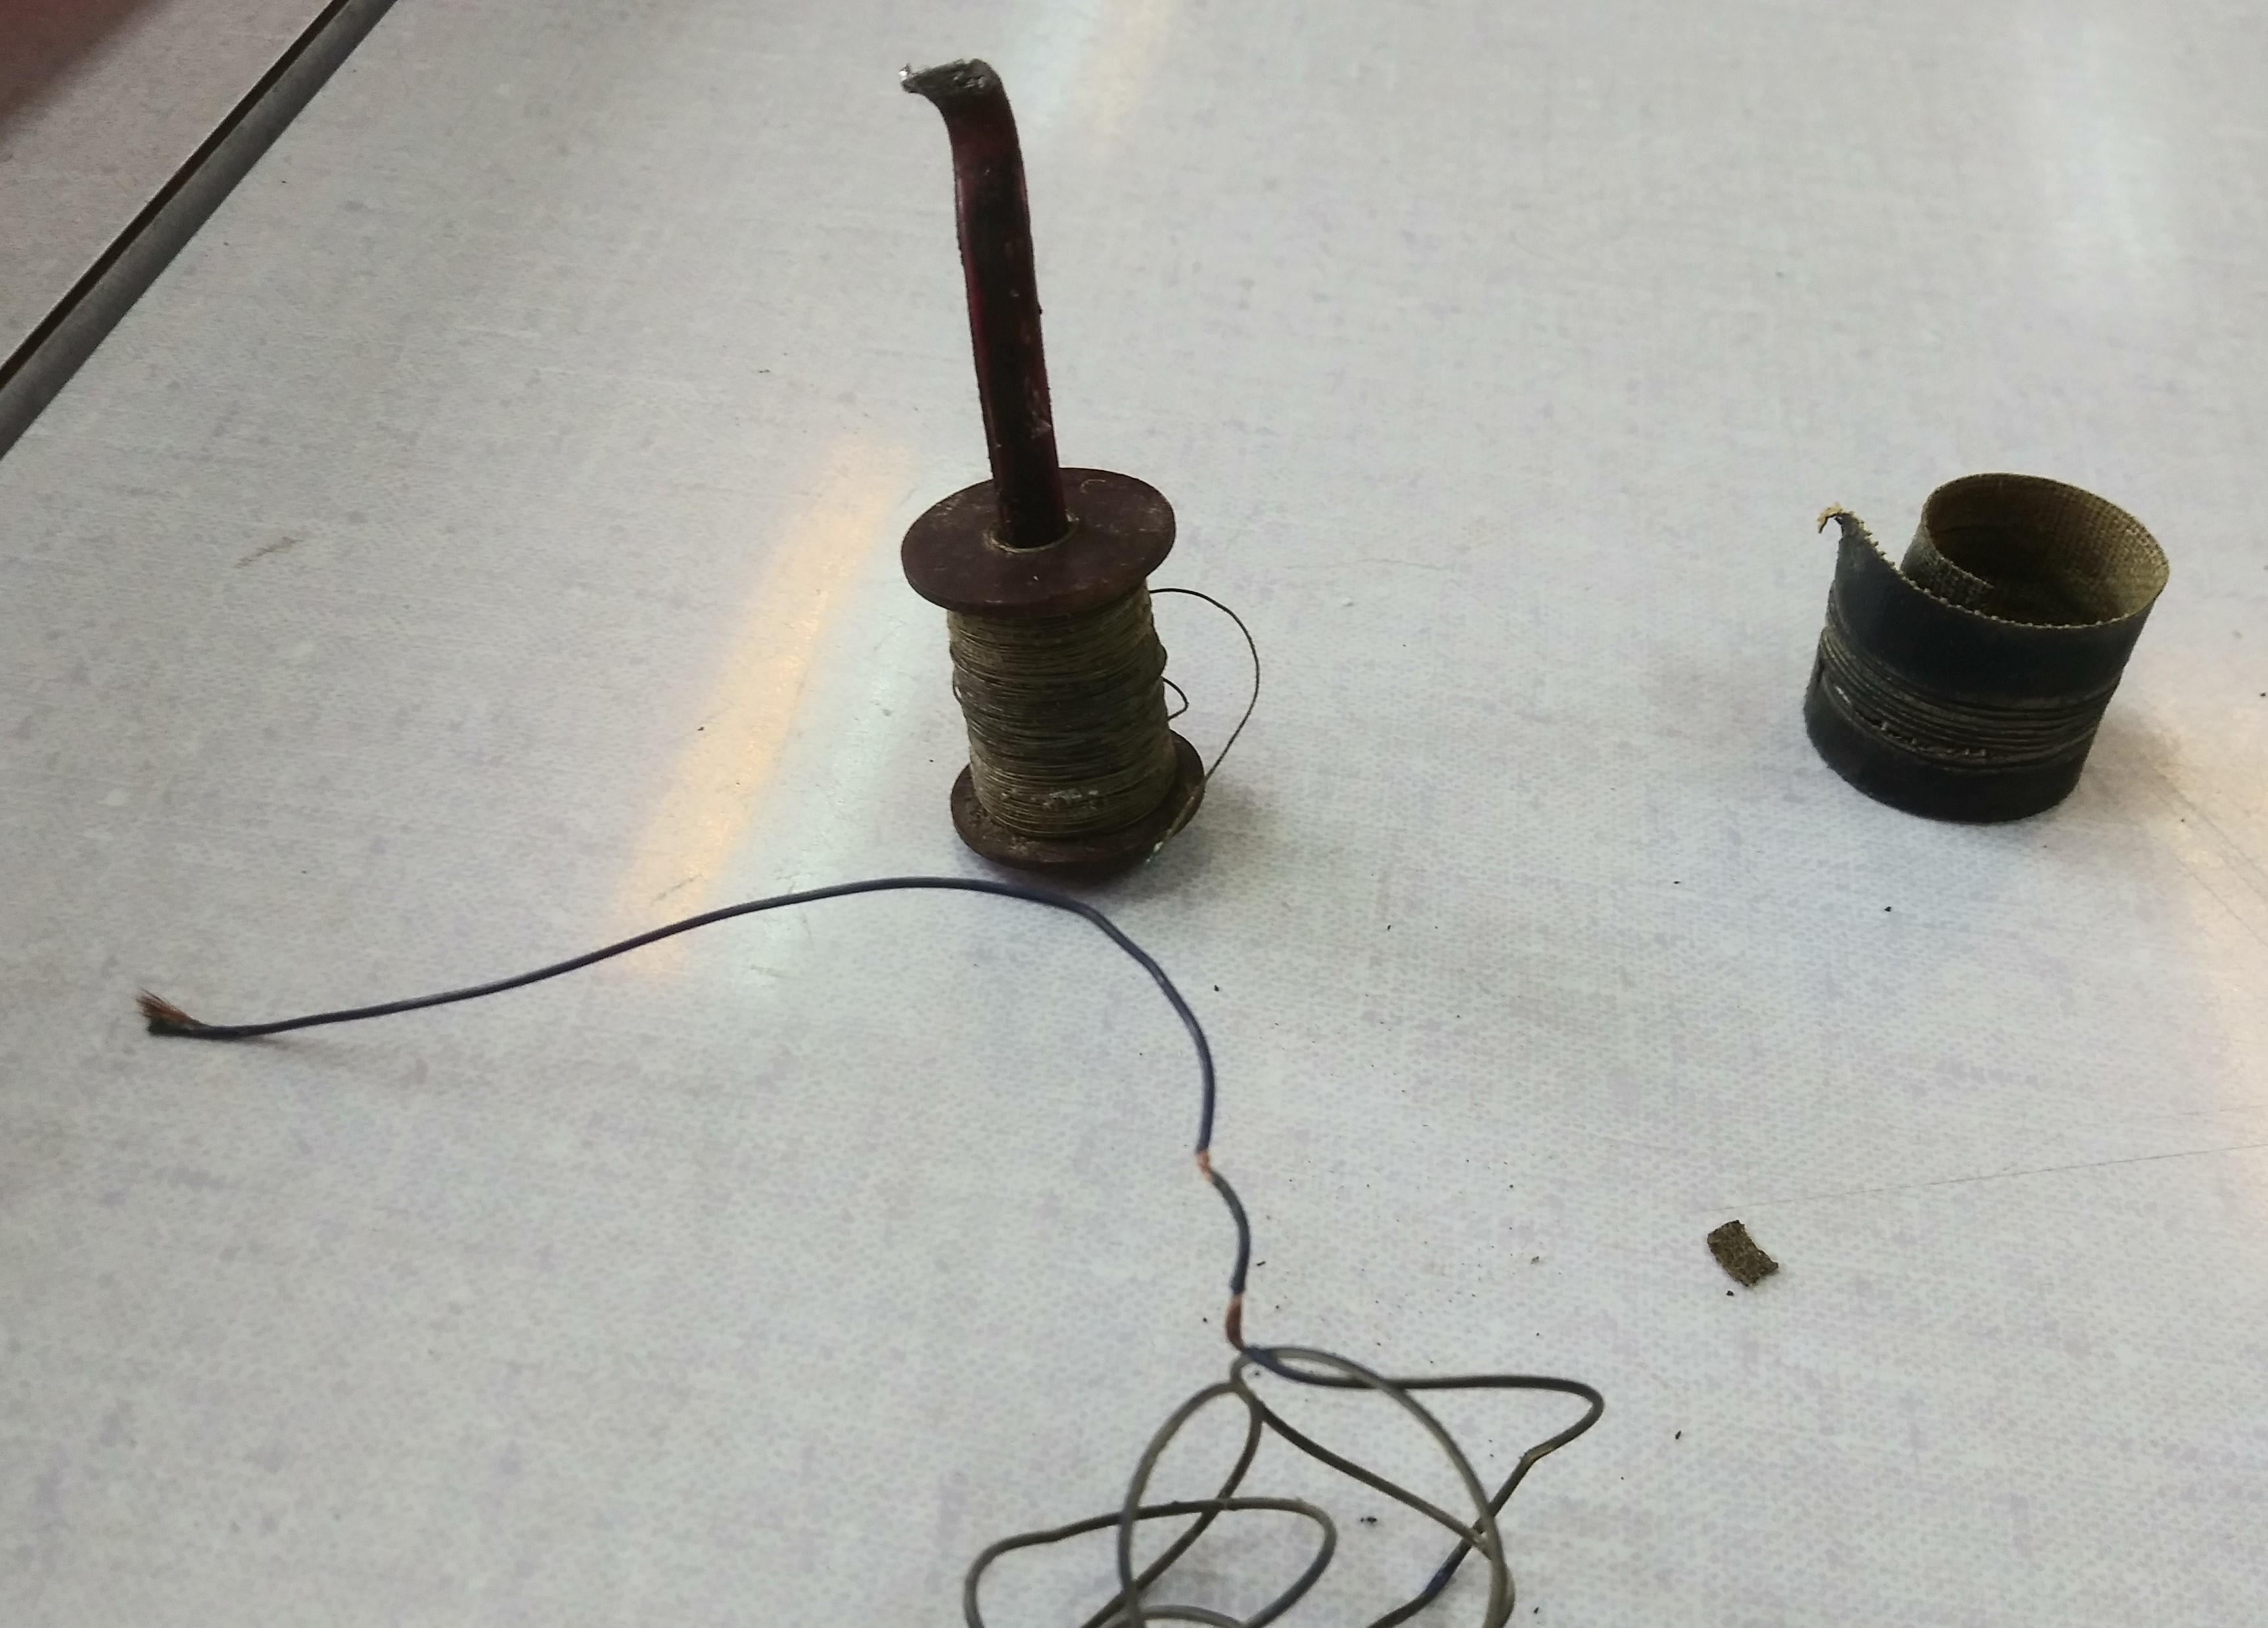
\includegraphics[height=300 pt]{images/20210311_150656.jpg}
    \caption{Une des trois bobines résistives sur sa broche de cuivre.
    On voit à droite la bande de maintien de la bobine et en bas, le fil de cuivre isolé qui relie les bobines entre elles.}
    \label{fig:bobine}
\end{figure}

Lors du déroulage du fil résistif, nous avons observé à plusieurs endroits que le fil était cassé, ce qui explique que l'appareil ne soit plus fonctionnel.
Nous avons aussi constaté que le fil métallique de couleur grise est isolé par un fil de soie très fin enroulé autour.
Les fils de plus gros diamètre, qui relient les bobines entre elles sont des fils de cuivre isolés.
Le fil résistif est maintenu en bobine par une bande isolante collante de couleur marron enroulée sur la bobine, seul le fil de cuivre isolé entre les bobines est visible une fois la bande collante mise en place.

\subsubsection{Caractérisation des bobines}

On s'intéresse au bobinage résistif correspondant au premier calibre du voltmètre (calibre \SI{1.5}{V}, résistance affichée \og R = 500\fg{}).
Le protocole précédemment détaillé est appliqué à cette bobine pour la caractériser.
Voici le compte-rendu des observations réalisées.

Il y a sept tours de fil de cuivre tressé au-dessus d'un tour de ruban adhésif en toile puis un fil plus fin entouré de fil de soie.
On déroule la bobine en comptant le nombre de tours : il y a 680 tours.
La longueur totale du fil est mesurée avec un décamètre dans le couloir : le fil fin mesure \SI{21.8(2)}{m}.

On mesure la résistance $R$ du fil pour quelques longueurs de fil :
\begin{itemize}
\item pour \SI{1}{m} : on mesure la résistance d'un mètre de fil avec un multimètre $ R = \SI{16.6(2)}{\ohm}$ ;
\item pour \SI{10}{m} : on mesure la résistance de dix mètres de fil avec le multimètre $ R = \SI{177(5)}{\ohm} $.
\end{itemize}

La section du fil est mesurée avec un pied à coulisse puis avec un micromètre : on trouve \SI{200}{\micro\metre} à plusieurs endroits du fil (sans la soie).
Le rayon $r$ du fil résistif est donc proche de \SI{100}{\um} pour cette bobine.

Avec ces mesures on peut finalement estimer la résistivité $\rho$ du matériau utilisé pour le fil :
\[
\rho = R \frac{\pi r^2}{l}
\]
et on trouve $\rho \sim \SI{50e-8}{\ohm\cdot\meter}$.
Cette mesure de la résistivité du matériau ainsi que la couleur du métal plutôt grise nous fait dire que le fil résistif est probablement fait de constantan (alliage de cuivre et de nickel) \cite{res_fil}.
La résistance totale de la bobine est par ailleurs estimée à $21{,}8 \times 17{,}7 \sim \SI{390}{\ohm}$.

Ces mesures sont répétées pour les deux autres bobines (cassées également) ce qui permet d'obtenir les valeurs estimées du tableau~\ref{tab:bobines}.

\begin{table}[htbp]
    \center
    \begin{tabular}{l|c|c|c}
    & \textbf{Bobine 1} & \textbf{Bobine 2} & \textbf{Bobine 3} \\
    \hline \hline
    \textbf{Diamètre du fil} (\unit{\um})                           & \num{200} & \num{200}   & \num{100} \\
    \textbf{Longueur du fil} (\unit{m})                             & \num{21,8} & \num{37}    & \num{78}\\
    \textbf{Résistance linéique} (\unit{\ohm\per\metre})& \num{17}    & \num{13}    & \num{46}\\
    \textbf{Résistance totale estimée} (\unit{\ohm})       & \num{386}  & \num{480}  & \num{3600}\\
    \end{tabular}
    \caption{Bilan des mesures réalisées permettant d'estimer les caractéristiques des bobines résistives.
    D'après nos observations, tous les fils résistifs sont en constantan.}
    \label{tab:bobines}
\end{table}

La mesure du diamètre du fil est délicate.
Nous avons aussi tenté de mesurer sa dimension en exploitant le phénomène de diffraction : un faisceau laser illumine le fil et on observe sur un écran éloigné une figure de diffraction.
La taille de la tache centrale pourrait nous indiquer précisément la taille du fil puisque l'on connait la longueur d'onde du laser.
Cette mesure réalisée à la hâte n'a cependant pas donné de résultats satisfaisants et devrait être répétée.

\subsubsection{Test fonctionnel}

Nous décidons de faire un test fonctionnel de l'appareil en utilisant des résistances modernes pour remplacer les bobines résistives.
Nous choisissons une association de trois résistances correspondantes aux indications du cadran de l'appareil (Fig.~\ref{fig:galva_volt_res}), soit :
\begin{align*}
R_1 &= \qty{500}{\ohm} \quad (\qty{200}{\ohm} +\qty{150}{\ohm} + \qty{150}{\ohm}) ;\\
R_2 &= \qty{500}{\ohm} \quad (\qty{250}{\ohm} + \qty{250}{\ohm} \text{ et } R_1 + R_2 = \qty{1000}{\ohm}) ;\\
R_3 &= \qty{4000}{\ohm} \quad (\qty{2000}{\ohm} + \qty{2000}{\ohm} \text{ et } R_1 + R_2 + R_3 = \qty{5000}{\ohm}).
\end{align*}

\begin{figure}[htbp]
    \center
    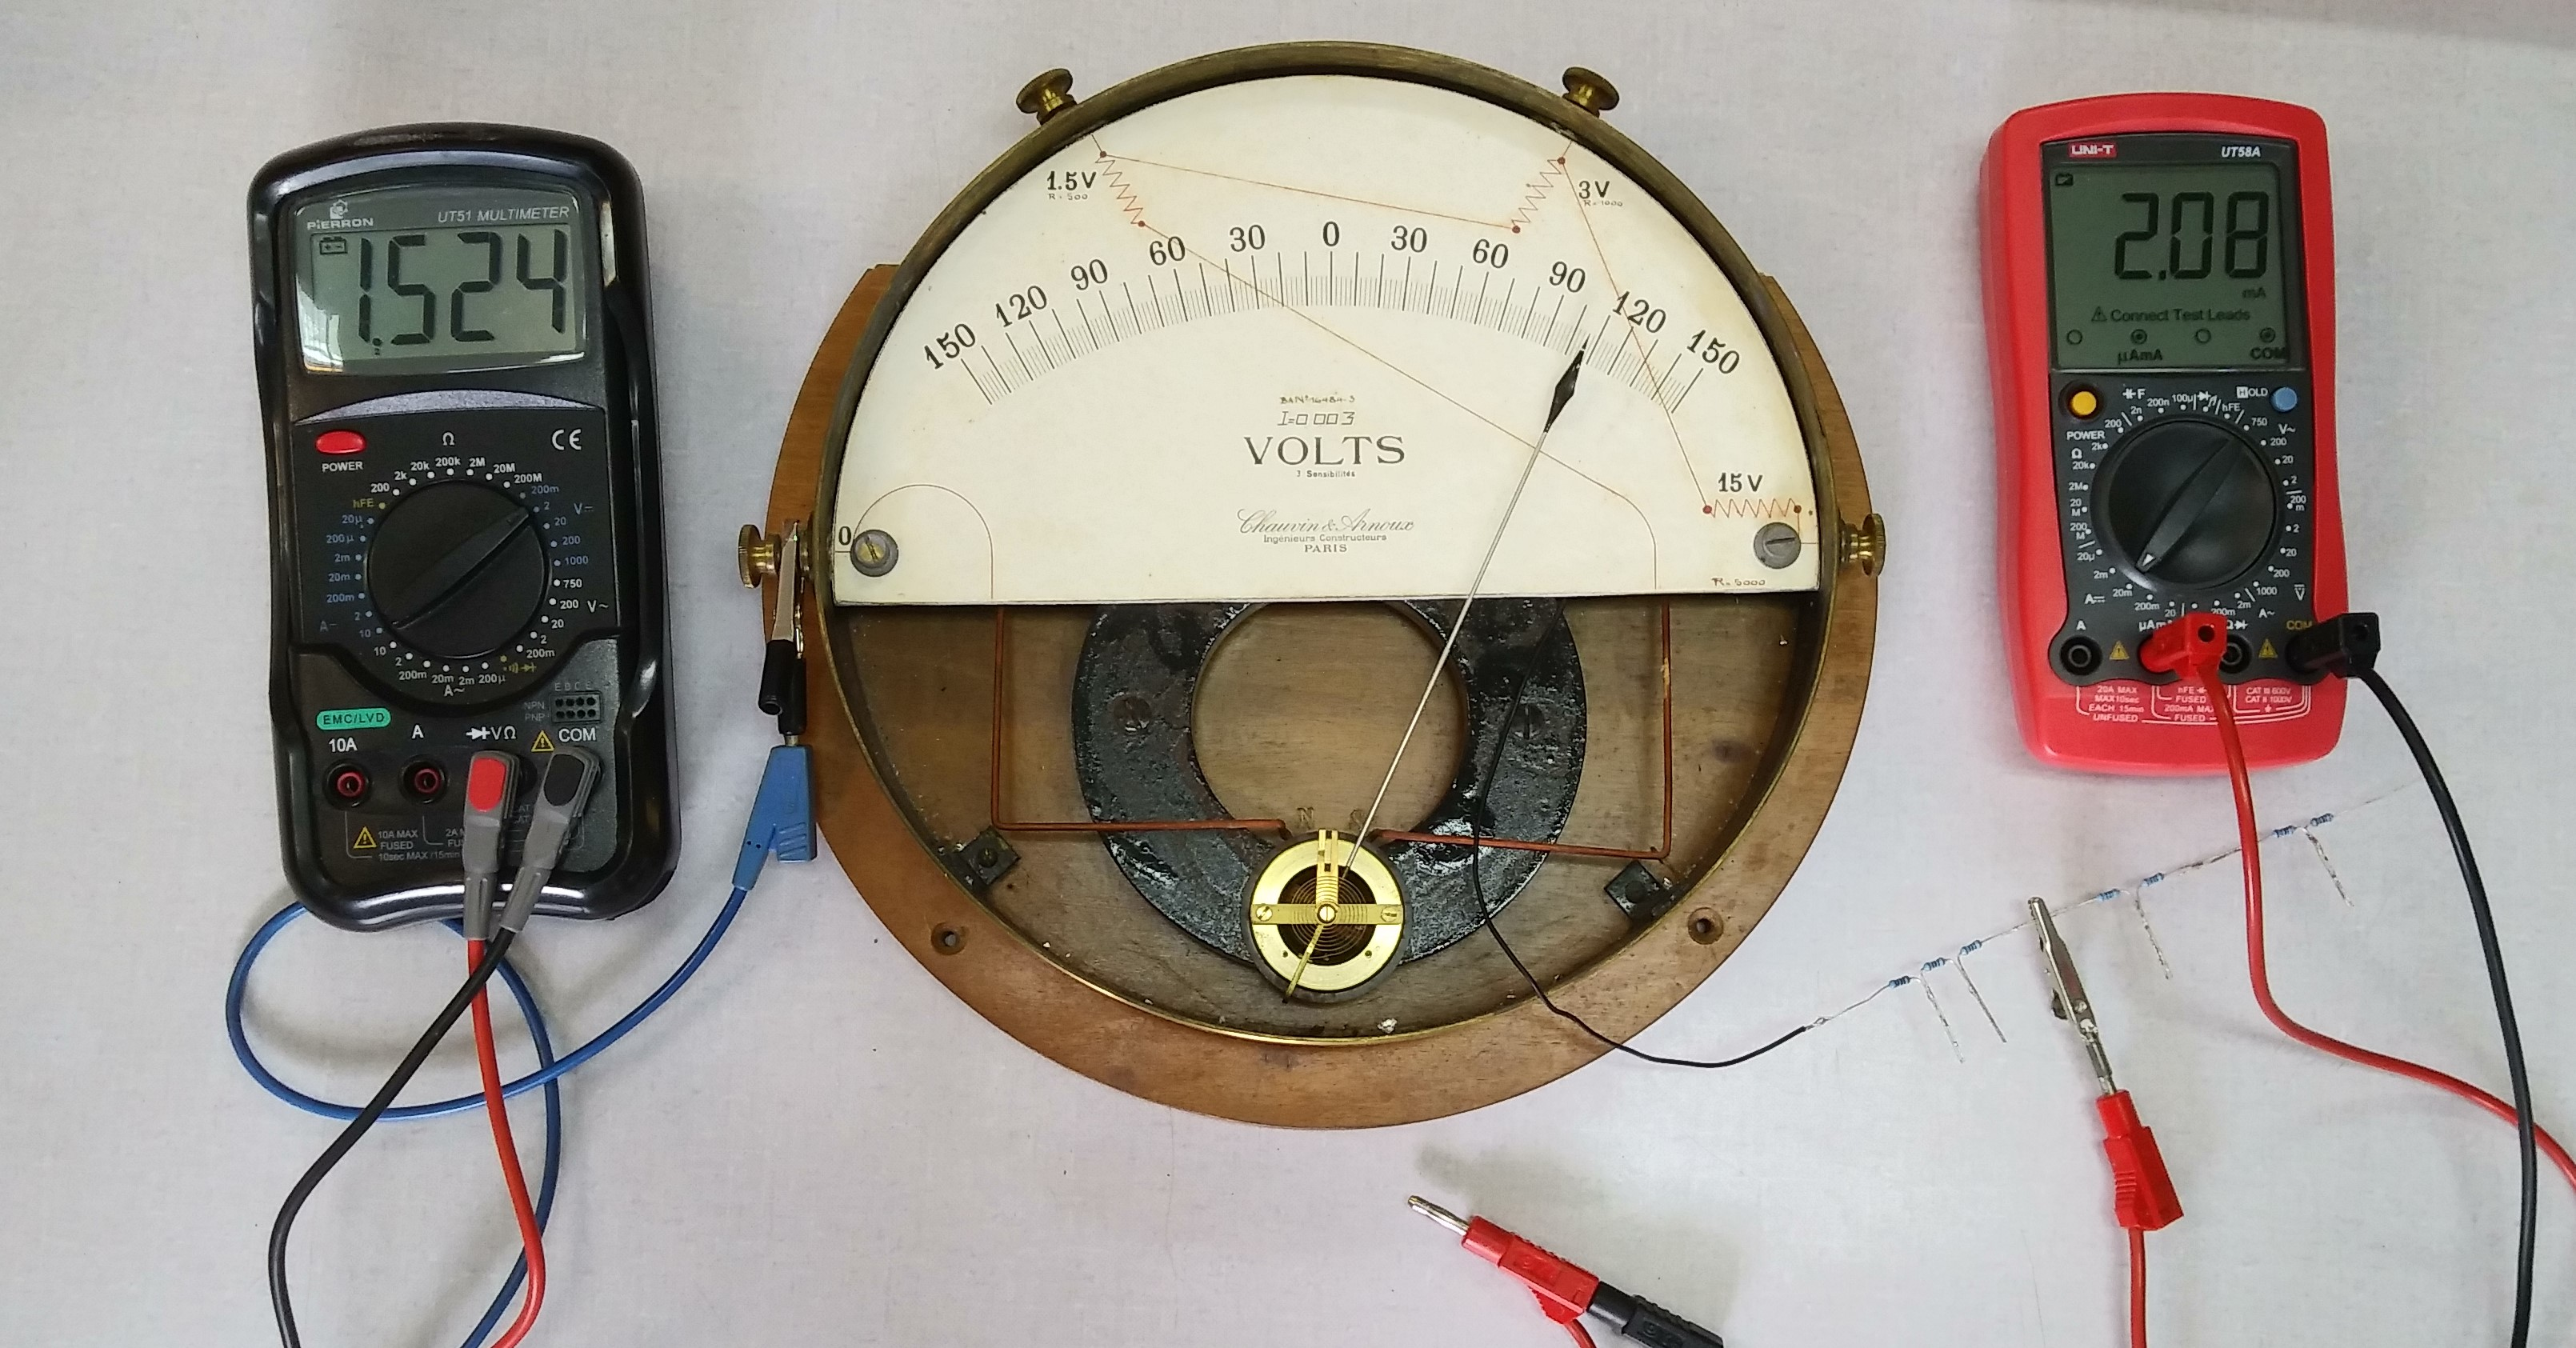
\includegraphics[width=\linewidth]{images/20210312_112248.jpg}
    \caption{Test de mesure pour une tension de \qty{1,5}{V} sur le calibre $R_1 = \qty{500}{\ohm}\ (\qty{150}{\ohm} + \qty{150}{\ohm} + \qty{200}{\ohm})$.}
    \label{fig:galva_volt_res}
\end{figure}
Pour la mesure, nous réalisons un pont diviseur de tension, alimenté par un générateur de tension réglable.
Un multimètre (noir) mesure la tension aux bornes du pont diviseur de tension : c'est grâce à cette mesure que nous ajustons la tension que le galvanomètre va mesurer.
Le galvanomètre est branché lui aussi aux bornes du pont diviseur de tension, en série avec un multimètre qui nous permet de vérifier l'intensité du courant circulant dans le galvanomètre.
Nous décidons de commencer les mesures en utilisant le plus petit calibre de l'appareil, nous devons donc utiliser seulement la résistance $R_1$, en série avec la bobine du cadre mobile.
Une fois la tension de \qty{1,5}{V} appliquée aux bornes du pont diviseur de tension, nous constatons que l'aiguille indique la graduation 106, et pas la graduation 150 comme nous l'espérions.

Une rapide application de la loi d'ohm pour la boucle du galvanomètre nous donne une résistance plus grande que \qty{500}{\ohm} :
\[
R = \frac{U}{I} = \frac{\num{1,524}}{\num{2,08e-3}} = \qty{732}{\ohm}.
\]
Nous décidons donc de vérifier la résistance totale du galvanomètre en utilisant un ohmmètre. 
Entre la résistance $R_1$ et la borne 0 nous mesurons \qty{650}{\ohm}, la valeur est plus élevée que la résistance $R_1$ seule, mais pas égale à \qty{732}{\ohm}. 
La première erreur est d'avoir utilisé de trop grandes longueurs de fil entre les appareils, l'addition des résistances bien que faibles des fils donne vite une erreur systématique de plusieurs dizaines d'ohms.
La deuxième erreur, la plus importante, est que nous n'avons pas pris en compte la résistance de la bobine du cadre mobile que nous mesurons à \qty{150}{\ohm}. 
Le document constructeur des appareils de 1915 (Ann.~\ref{ann:catalogue}) fait mention d'une résistance interne de \qty{75}{\ohm} en moyenne pour la bobine du cadre mobile, cette valeur semble cohérente avec ce que nous observons. 
Afin de prendre en compte cette résistance interne de l'appareil, nous changeons la valeur de la résistance $R_1$ pour que la valeur totale de $R_1$ et de la bobine du cadre mobile soit égale à \qty{500}{\ohm}.

On modifie donc la valeur de $R_1$ à \qty{350}{\ohm} ($\qty{200}{\ohm} + \qty{150}{\ohm}$ et $R_1 + R_\mathrm{cadre\ mobile} = \qty{500}{\ohm}$).
Nous menons à nouveau l'expérience précédente, en minimisant les longueurs de fils de connexion.
Cette fois, en appliquant une tension de \qty{1,5}{V}, l'aiguille du galvanomètre pointe exactement sur la graduation \num{150} et l'intensité traversant l'appareil est bien de \qty{3}{mA} (Fig.~\ref{fig:galva_volt_good}).

\begin{figure}[htbp]
    \center
    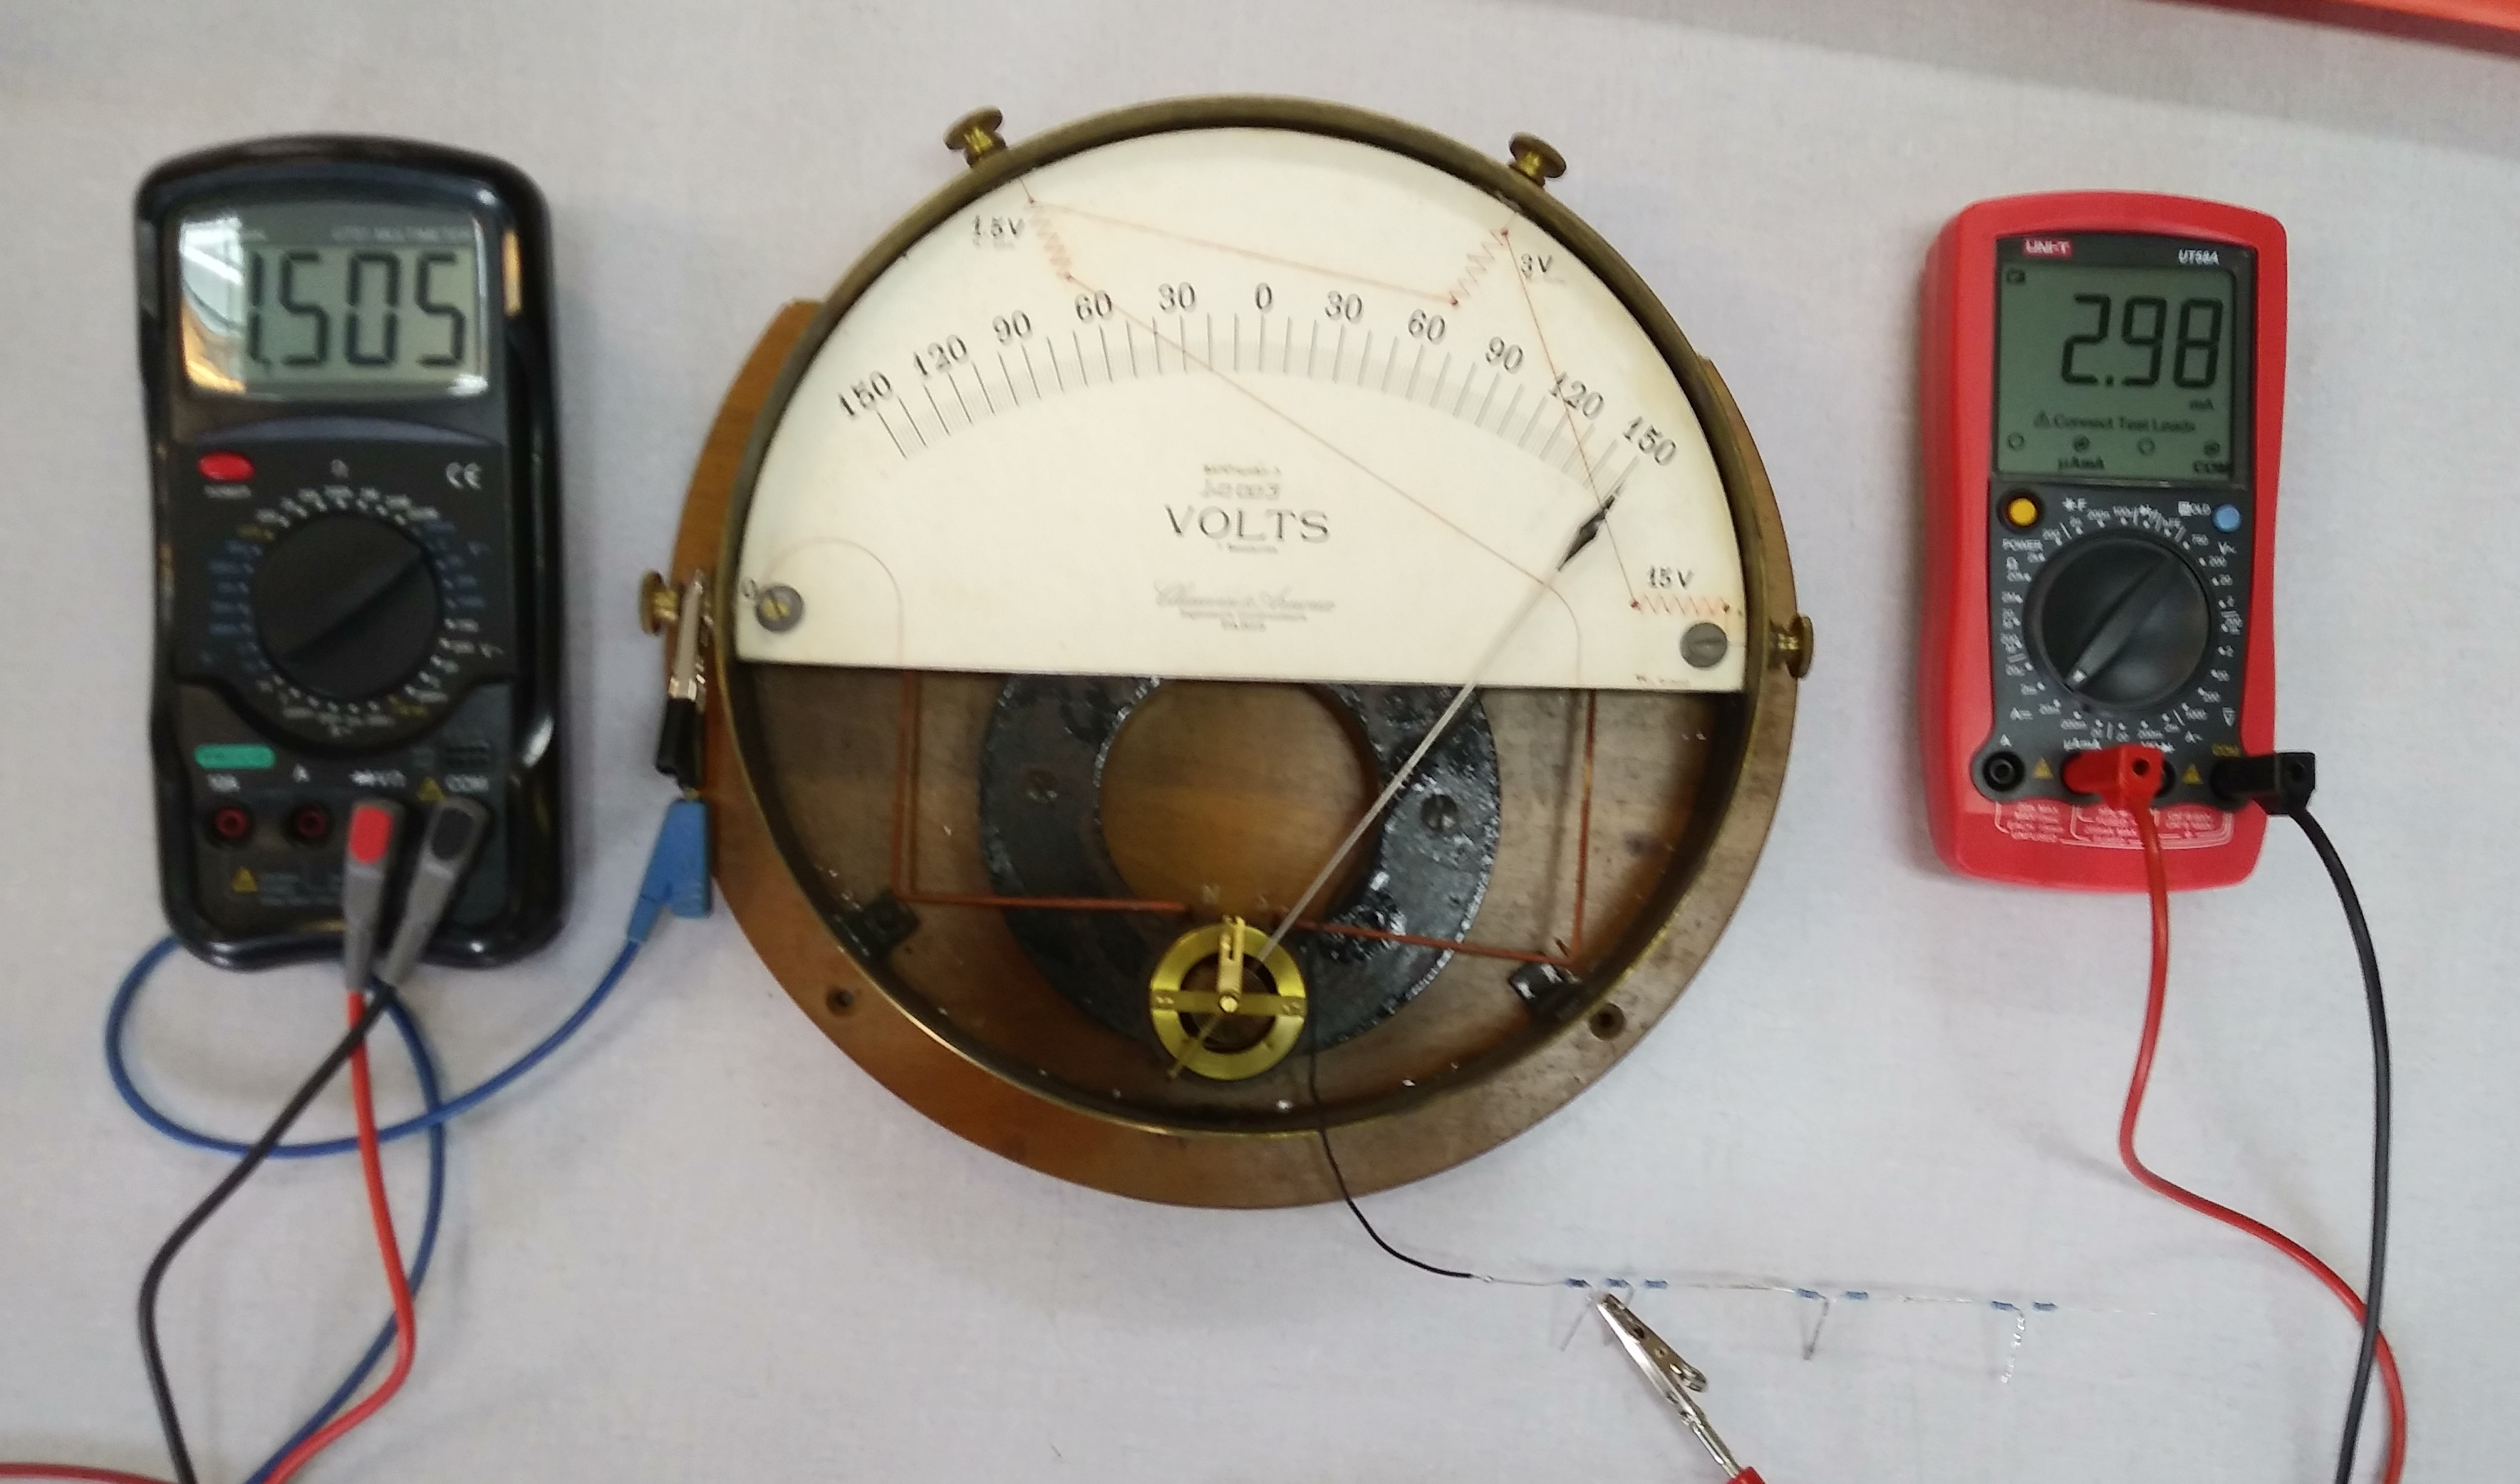
\includegraphics[width=\linewidth]{images/20210312_112818.jpg}
    \caption{Test de mesure pour une tension de \qty{1,5}{V} sur le calibre $R_1 = \qty{350}{\ohm}$ ($\qty{150}{\ohm} + \qty{200}{\ohm}$).
    \label{fig:galva_volt_good}
}
\end{figure}

Cette dernière expérience est bien conforme à l'utilisation prévue par le constructeur : \og Dans les voltmètres, le circuit du cadre mobile à une résistance moyenne de 75 ohms, et un courant de 5 milliampères (0.005) suffit pour donner à l'aiguille une déviation égale à la totalité de l'échelle.
À la suite du cadre mobile, sont placées en série, avec lui, des bobines dont la résistance ne varie pas avec la température et dont la valeur est proportionnelle à la f. e. m. maxima à mesurer. \fg{}
Pour notre appareil les valeurs sont de \qty{150}{\ohm} pour la résistance du cadre mobile et de \qty{3}{mA} pour la déviation maximale.

\subsection{Remontage de l'appareil}
\label{sec:remontage_volt}

À ce stade, nous avons deux options pour le remontage de l'appareil :
\begin{itemize}
\item remise en état à l'identique avec des matériaux neufs pour reconstruire les bobines résistives ;
\item remise en état fonctionnelle à l'identique en utilisant des résistances à semi-conducteurs modernes en remplacement des bobines résistives.
\end{itemize}
Notre objectif premier était de pouvoir remonter les bobines résistives avec des matériaux neufs.
Cependant malgré les recherches de fournisseurs de fils résistifs en constantan ou autre alliage aux propriétés comparables, nous n'avons pas réussi à trouver un fournisseur capable de répondre à nos besoins très spécifiques.
La problématique majeure pour eux étant de nous fournir de très petites quantités, comparées à leur échelle industrielle de fabrication.
En effet, nous avons eu plusieurs propositions pour nous fournir des kilogrammes de bobines de fils résistifs en constantan alors que notre besoin est de l'ordre de quelques dizaines de grammes par bobine dans l'appareil.
L'offre étant beaucoup trop disproportionnée par rapport à nos besoins, nous avons choisi d'utiliser des semi-conducteurs modernes pour faire fonctionner l'appareil.

D'un point de vue purement fonctionnel, l'utilisation de résistances modernes n'impacte en rien le fonctionnement original de l'appareil.
Dans la conception de l'appareil, les bobines résistives avaient pour seul et unique rôle de fournir une résistance électrique constante avec la température.
\footnote{À ce titre, les résistances choisies ont une dépendance certaine avec la température qui peut nuire à la précision de l'appareil.
Toutefois ces variations restent faibles.}
L'appareil était d'ailleurs conçu de manière telle que les champs magnétiques induits par ces bobinages ne puissent pas influencer le mouvement de l'aiguille du cadre mobile.
Les résistances choisies pour les différents calibres sont les suivantes (Fig.~\ref{fig:galva_volt_mod}) :
\begin{itemize}
\item équivalents de la bobine résistive 1 : \qty{350}{\ohm} (deux résistances de \qty{150}{\ohm} en série suivies de deux résistances de \qty{100}{\ohm} en parallèle) ;
\item équivalents de la bobine résistive 2 : \qty{500}{\ohm} (deux résistances de \qty{500}{\ohm} en série) ;
\item équivalents de la bobine résistive 3 : \qty{4000}{\ohm} (deux résistances de \qty{2000}{\ohm} en série).
\end{itemize}

\begin{figure}[htbp]
    \center
    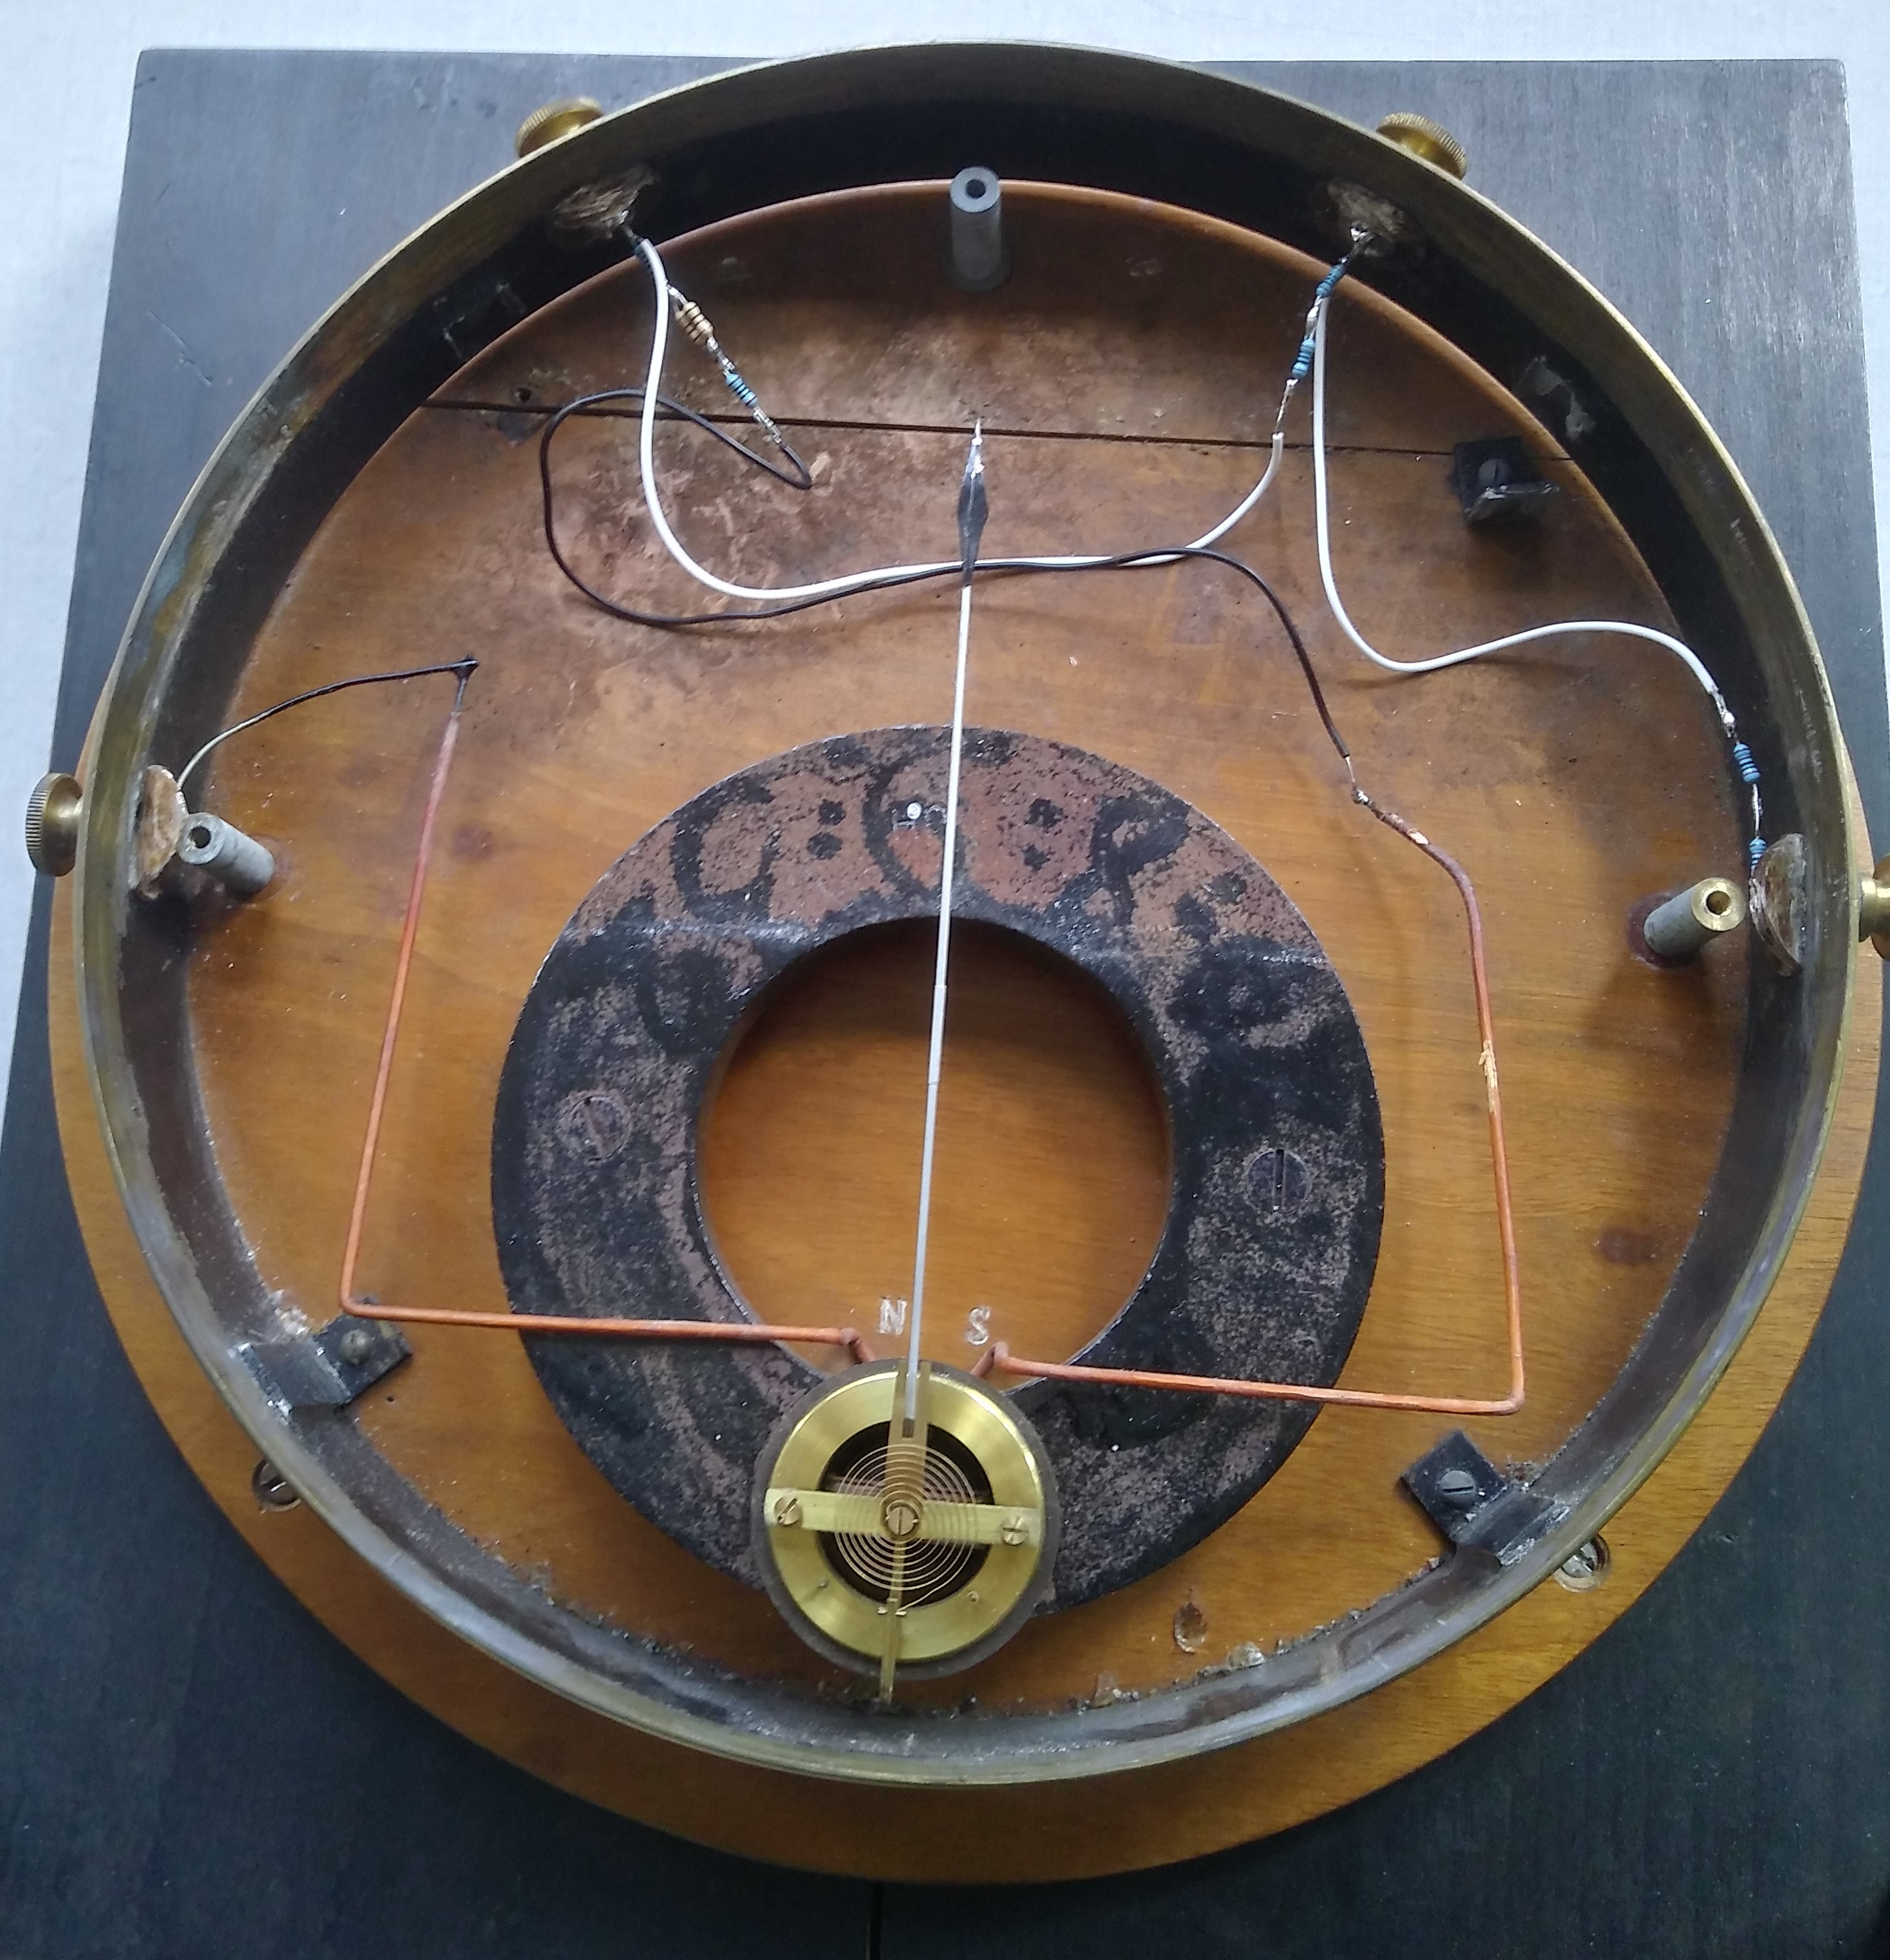
\includegraphics[height=300 pt]{images/20210505_155742_HDR.jpg}
    \caption{Remontage de l'appareil avec des résistances modernes.
    \label{fig:galva_volt_mod}
}
\end{figure}

Nous avons ensuite dépoussiéré et nettoyé sommairement les parties de l'appareil avant remontage comme à l'origine.
Il est nécessaire d'être minutieux lors du remontage de la vitre tout particulièrement en ce qui concerne l'insert de réglage du zéro.
Il faut placer l'axe derrière la vitre sur l'axe de symétrie de la vitre, et veiller à ce que le petit axe se place entre les deux languettes du dessus du cadre mobile.
Une fois la vitre positionnée, il faut régler le zéro de l'appareil et s'assurer que rien n'entrave la course de l'aiguille qui a un espace réduit de quelques millimètres pour se déplacer entre la vitre et le cadran.









\section{Un test de fonctionnement}

Avec les deux appareils remontés, nous réalisons un test rapide pour s'assurer que les appareils fonctionnent correctement.
Une expérience plus poussée permettant d'évaluer la précision des appareils n'a pu être réalisée par manque de temps.

Un générateur stabilisé en tension et possédant deux calibres (\qty{6}{V} et \qty{12}{V}) alimente une résistance de \qty{300}{\ohm}.
Le galvanomètre ampèremètre est branché en série avec la résistance et le galvanomètre voltmètre est branché aux bornes de la résistance (Fig.~\ref{fig:circuit}).
Ce denier est utilisé avec son plus gros calibre (\qty{15}{V}, résistance interne \qty{5000}{\ohm}).
On mesure donc simultanément le courant $I$ qui parcourt la résistance et la tension $U$ à ses bornes.
La loi d'ohm permet d'évaluer rapidement la cohérence des mesures obtenues en calculant le courant $I_\mathrm{ohm}$ attendu dans le circuit compte tenu des composants utilisés (Tab.~\ref{tab:mesures}).

\begin{figure}[htbp]
    \center
    \begin{circuitikz}
        \draw (0,0) to [vsource, v=\qty{6}{V} -- \qty{12}{V}, i=$I$] (0,3);
        \draw (0,3) to [rmeter, t=A] (3,3);
        \draw (3,3) to [R, l=$R$, v=$U$] (3,0);
        \draw (3,0) -- (0,0);
        \draw (3,3) -- (5,3) to [rmeter, t=V] (5,0) -- (3,0);
    \end{circuitikz}
    \caption{Circuit utilisé pour les mesures.}
    \label{fig:circuit}
\end{figure}

\begin{table}[htbp]
    \center
    \begin{tabular}{c|c|c|c|c|c|c}
        \textbf{Tension du générateur} & \multicolumn{2}{c|}{\textbf{Tension} $U$} & \multicolumn{2}{c|}{\textbf{Courant} $I$} & \multicolumn{2}{c}{\textbf{Courant} $I_\mathrm{ohm}$} \\
        (\unit{\volt}) & (\unit{graduation}) & (\unit{\volt}) & (\unit{graduation}) & (\unit{\mA}) & (\unit{mA}) & corrigé (\unit{mA)} \\
        \hline \hline
        \num{12} & \num{120} & \num{12,0} & \num{128} & \num{42,7} & \num{40} & \num{42,4} \\
        \num{6} & \num{58} & \num{5,8} & \num{62} & \num{20,7} & \num{20} & \num{20,5} 
    \end{tabular}
    \caption{Mesures relevées lors du test de fonctionnement des appareils.
    La première colonne indique le calibre du générateur de tension.
    Les deux suivantes indiquent la valeur de tension relevée sur le galvanomètre voltmètre : la tension en volts se calcule à partir de la lecture sur l'appareil en tenant compte du calibre utilisé (ici, \qty{15}{V} correspond à la graduation \num{150}).
    Les deux d'après indiquent la valeur du courant mesuré avec le galvanomètre ampèremètre : le courant en ampère se calcule à partir de la lecture sur l'appareil (ici, \qty{0,050}{A} correspond à la graduation \num{150}).
    L'avant dernière colonne donne le courant estimé avec la loi d'ohm d'après le calibre du générateur.
    La dernière tient compte de la présence des différents appareils, notament de celle du voltmètre dont la résistance interne de \qty{5}{\kilo\ohm} affecte le montage.}
    \label{tab:mesures}
\end{table}

Avec ces résultats, on constate que les appareils fonctionnent convenablement : 
\begin{itemize}
\item la tension correspond à la valeur du calibre du générateur (il faudrait la mesurer avec précision pour établir une comparaison plus quantitative).
L'influence de l'ampèremètre sur le montage est négligeable, avec sa résistance interne de l'ordre du ohm ;
\item le courant mesuré est en très bon accord avec les valeurs attendues, notamment lorsqu'on tient compte de la présence du voltmètre qui perturbe la mesure.
En effet, sa résistance interne de \qty{5}{\kilo\ohm} n'est pas si grande par rapport à la résistance utilisée dans le montage.
Elle est bien plus faible que la résistance de nombreux appareils plus modernes ($\sim\qty{1}{\mega\ohm}$) et il faut la prendre en compte pour obtenir des résultats précis.
La résistance équivalente à l'ensemble \{$R$, galvanomètre\} est de \qty{283}{\ohm}, ce qui explique le courant légèrement plus important que celui attendu.
\end{itemize}
Si la présence de l'ampèremètre n'est pas source de perturbation majeure dans ce montage, le voltmètre affecte sensiblement la mesure.
Il convient de prendre en compte la totalité du montage lorsque des mesures précises sont prévues.






\section*{Conclusion}
\addcontentsline{toc}{section}{Conclusion}

Durant ce travail nous avons pu étudier en détail le fonctionnement de deux galvanomètres ampèremètre et voltmètre du début du XX\textsuperscript{ème} siècle et les remettre en état de fonctionnement.
Leur démontage a permis de mieux comprendre leur principe de fonctionnement et d'apprécier leur conception astucieuse, qui permet des mesures sensibles et précises.
Il est regrettable que la restauration des bobines résistives du voltmètre avec des matériaux neufs n'ait pas pu avoir lieu : l'obtention du fil résistif adapté est difficile compte tenu des faibles quantités dont nous avions besoin.
Les résistances utilisées sont des résistantes modernes, qui ne correspondent pas à l'époque de fabrication de l'appareil, mais l'appareil fonctionne selon ses caractéristiques d'origine.

D'un point de vue strictement personnel, nous restons impressionnés par la qualité de conception et de fabrication de ces appareils qui datent de près d'un siècle.
En effet, grâce à seulement quelques composants, un aimant permanent et quelques fils aux propriétés finement connues et ajustés à l'usage, les industriels de l'époque étaient capables de fabriquer des appareils de mesure fiables et robustes qui n'ont rien à envier aux appareils grand public modernes en termes de précision.
Les promesses du fabricants indiquées dans le catalogue se sont par ailleurs avérées complètement justifiées.

\begin{figure}[htbp]
    \center
    \begin{multicols}{2}
    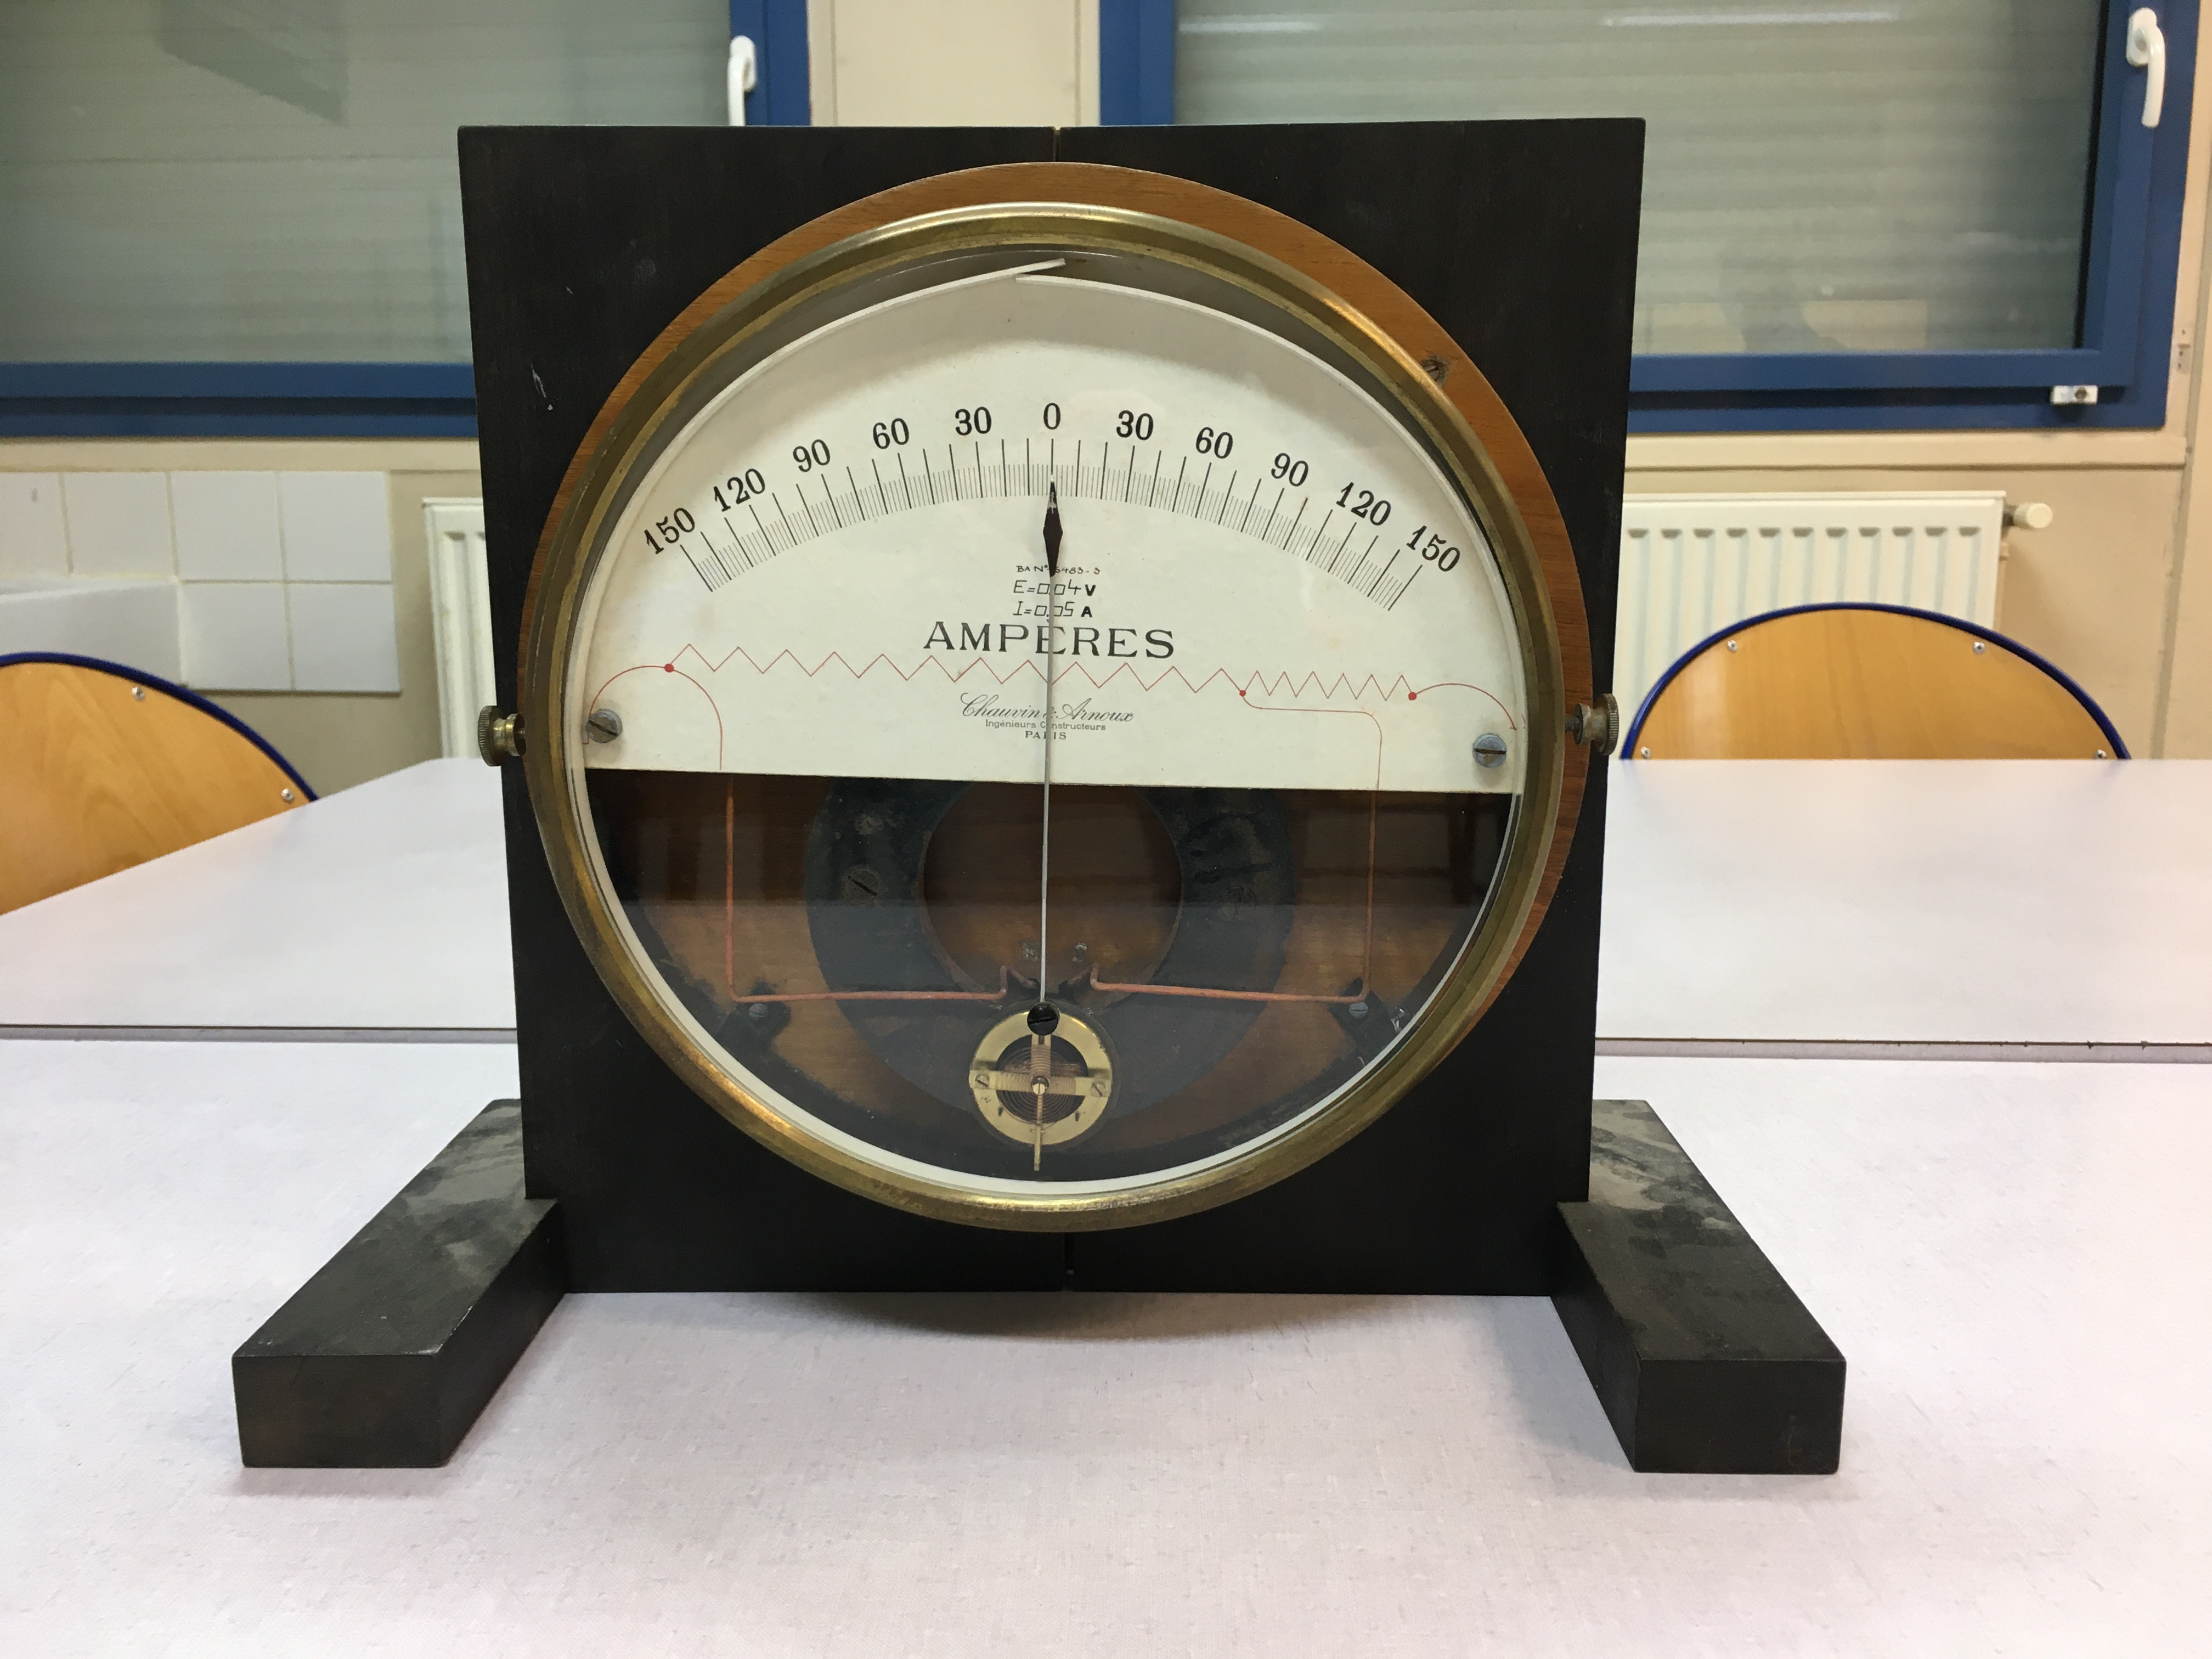
\includegraphics[width=\linewidth, trim=400 300 600 200, clip]{images/IMG_4045.JPG}
    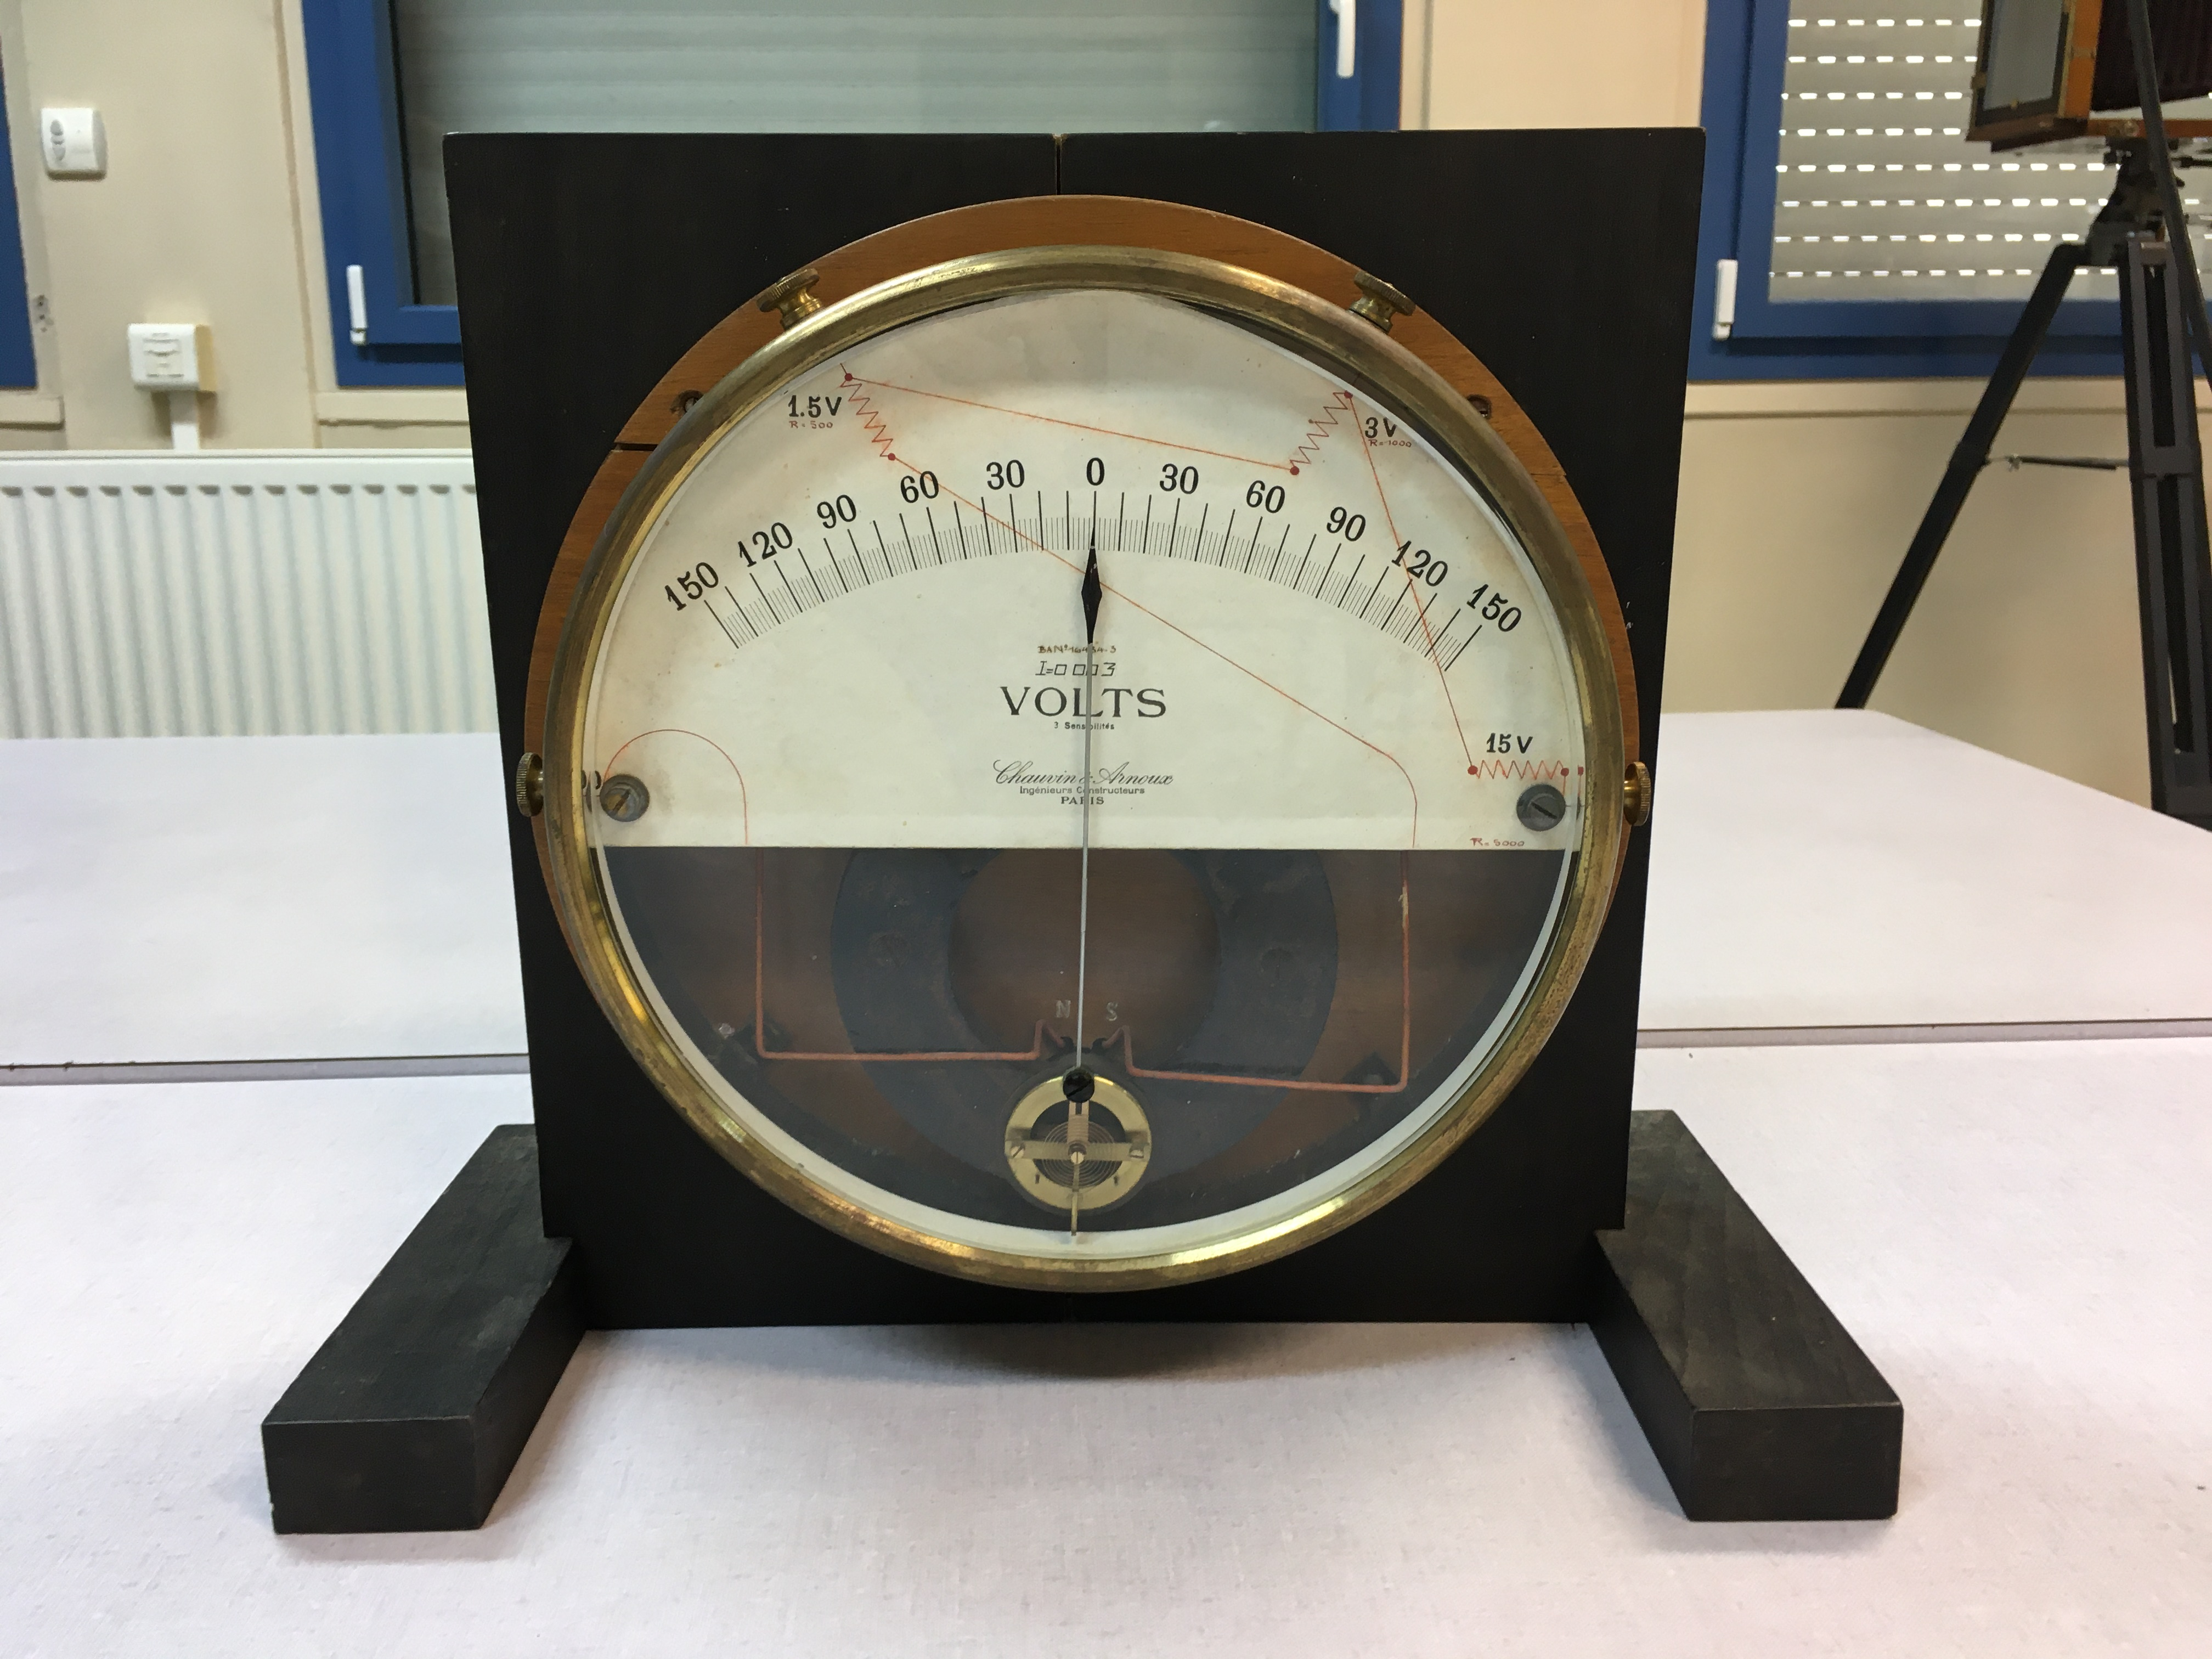
\includegraphics[width=\linewidth, trim=500 300 500 200, clip]{images/IMG_4047.JPG}
    \end{multicols}
    \caption{Les deux galvanomètres remis en état.}
\end{figure}






\newpage
\appendix

\bibliography{biblio.bib}
\addcontentsline{toc}{section}{Références}

\newpage
\appendix

\addcontentsline{toc}{section}{Annexes}

\section{Extraits du catalogue Chauvin \& Arnoux (1915)}
\label{ann:catalogue}

Le catalogue complet est disponible en cliquant sur le lien ci-dessous :

\noindent
\href{http://cnum.cnam.fr/CGI/fpage.cgi?M9857.1/1/100/137/104/135}{http://cnum.cnam.fr/CGI/fpage.cgi?M9857.1/1/100/137/104/135}

Les pages qui concernent les instruments étudiés dans ce rapport sont rapportées ci-après.

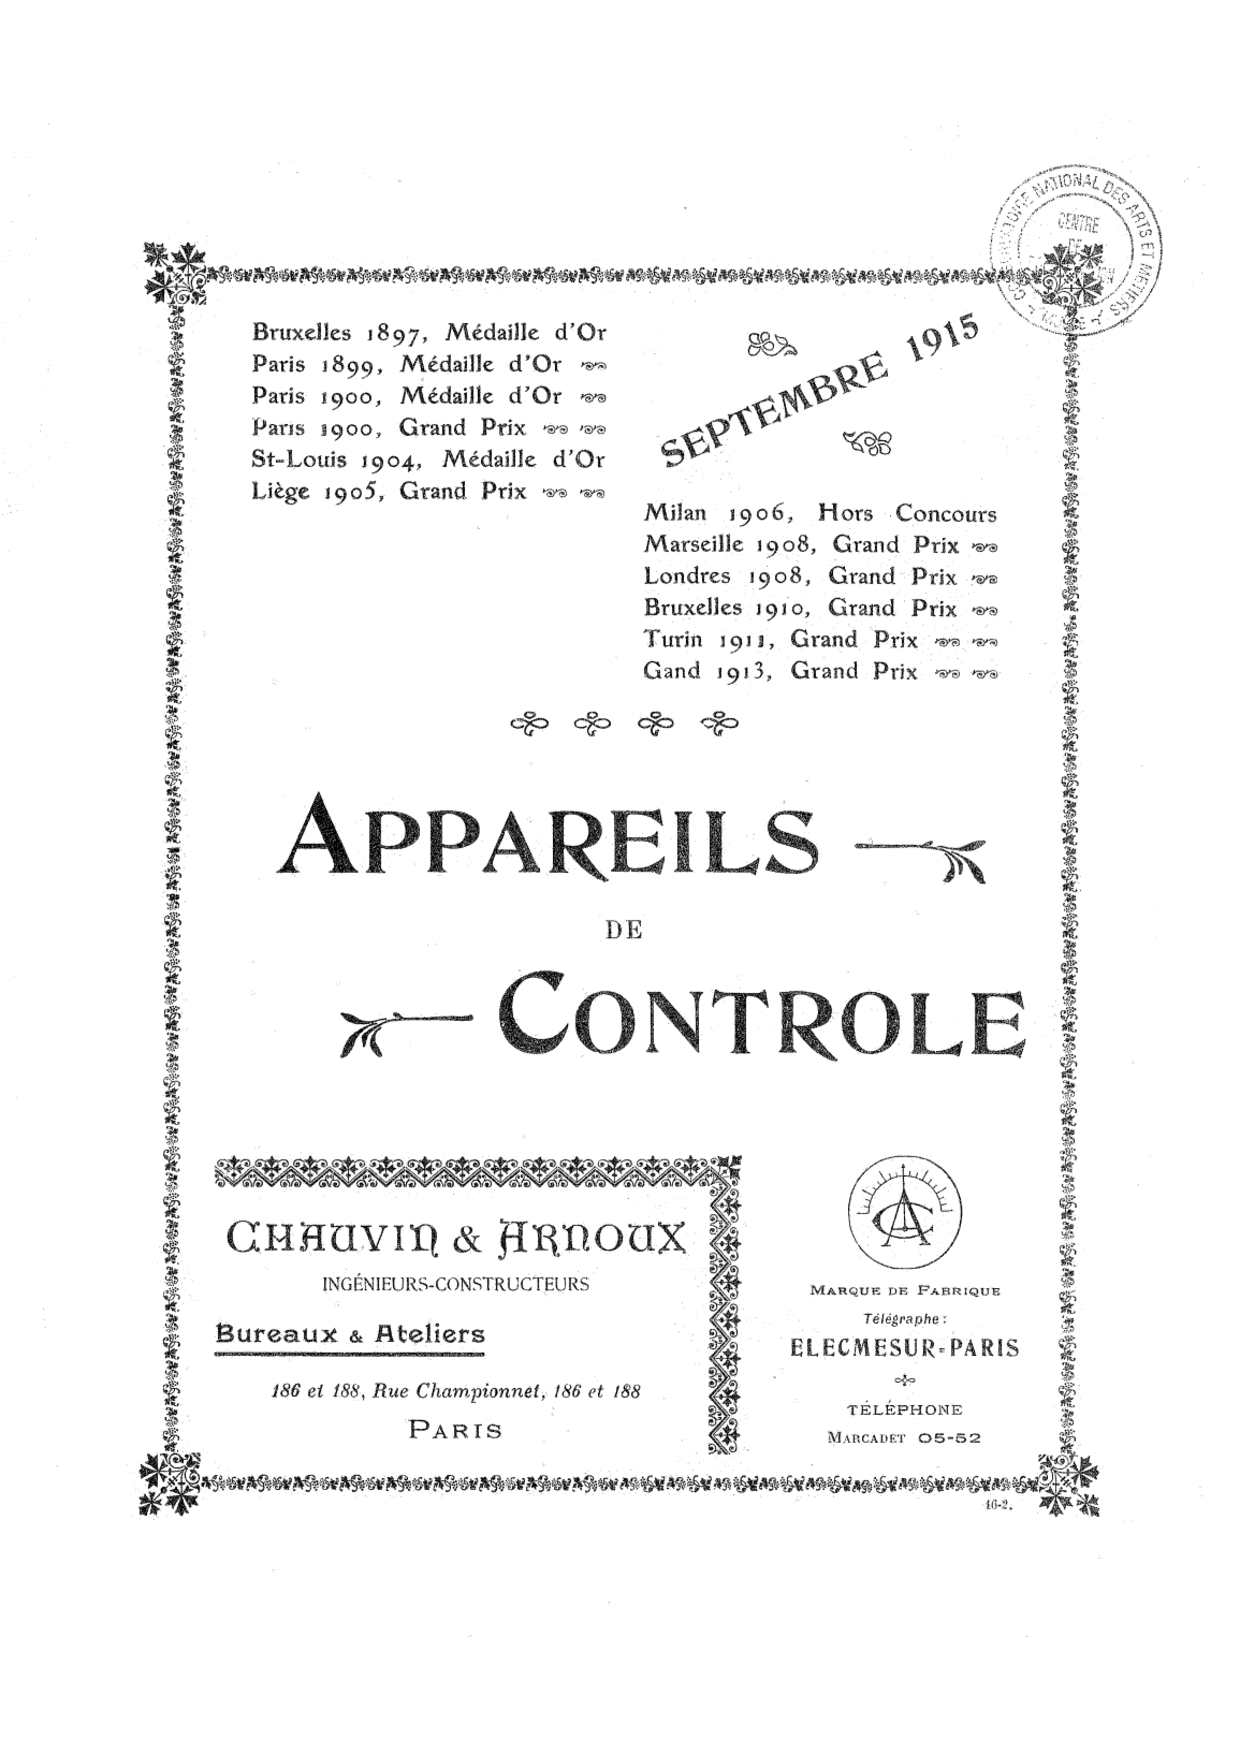
\includepdf[pages=-]{images/chauvin_arnoux.pdf}
\end{document}